% !TEX program = xelatex
\documentclass[UTF8,a4paper,12pt]{ctexart}
\usepackage{geometry}
\geometry{left=2.2cm,right=2.2cm,top=2.5cm,bottom=2.5cm}
\usepackage{amsmath,amssymb,bm}
\usepackage{graphicx}
\usepackage{booktabs,array,multirow}
\usepackage{subcaption}
\usepackage{enumitem}
\usepackage{float}
\usepackage{hyperref}
\hypersetup{hidelinks}
\graphicspath{{exp2_images/}}
\newcommand{\blank}[1][2.5cm]{\mbox{\underline{\hspace{#1}}}}
\newcommand{\answer}{\par\noindent\textbf{填写：}\blank[0.86\textwidth]\par}
\numberwithin{equation}{section}

\title{《超声波测试实验》实验报告}
\author{姓名\blank[2.5cm] \quad 学号\blank[3cm] \quad 同组成员\blank[4cm]\\[1em]
实验地点\blank[3cm] \quad 实验日期\blank[4cm]}
\date{}
\begin{document}
\maketitle
\tableofcontents
\clearpage

\section{实验目的}
\begin{enumerate}
  \item 掌握超声波传播基本知识及超声脉冲--回波检测原理。
  \item 了解脉冲发射接收仪的操作使用。
  \item 掌握超声波实验测波速、材料常数及衰减系数的基本方法。
  \item 了解 B-Scan 超声测试方法，以及焊缝缺陷的探测方法。
\end{enumerate}

\section{实验装置、仪器及器材}
\begin{enumerate}
  \item 超声脉冲发射接收仪（Olympus 5077PR Square Wave Pulser/Receiver）。
  \item 数字存储示波器（Tektronix DPO 3034 Digital Phosphor Oscilloscope）。
  \item 笔记本电脑（Lenovo Thinkbook 16p Gen 2）及示波器配套软件。
  \item Olympus NDT 5 MHz 水浸式超声探头、5 MHz 横波探头、5 MHz 及 10 MHz 纵波探头、1 MHz 斜探头。
  \item 试件：圆柱状钢制试件、圆柱状铝制试件、板状有机玻璃试件、带焊缝的钢板。
  \item 探头线、水盆、酒精、脱脂棉、纵波耦合剂（SF-CORES 医用超声耦合剂）、横波耦合剂（Olympus SWC-2 横波耦合剂）。
  \item 天平（BSM620.3 电子天平）、游标卡尺（桂林量具刃具有限责任公司制 0--150 mm 游标卡尺，50 分度）、钢制直尺（Stanley 35-345-23）。
\end{enumerate}

\section{实验测量方法与测量过程}
\subsection{超声波法测量材料动态力学性能的方法}
超声波是指振动频率大于 20 kHz 的声波。由于其每秒振动次数（频率）甚高，超出人耳听觉上限（20 kHz），人们将这种听不见的声波叫做超声波。超声波和可闻声波本质上是一致的，都是一种机械振动，通常以波的方式在弹性介质中传播。其不同点是超声频率高、波长短，在一定距离内具有良好的指向性。超声波的波速取决于弹性介质的力学性质。超声波在传播过程中会由于材料非均匀性的散射和吸收导致能量衰减，并且衰减会随着频率升高而快速增加。

超声波在材料性能测试、厚度测试及无损检测中具有广泛的应用。常用的脉冲--回波方法的基本原理如图\ref{fig:exp2-pulse-echo}所示，它利用超声传感器发射并接收反射回波信号。当采用超声传感器发射一个脉冲信号，经过试件上下表面多次反射，可得到相应的回波信号。通过对实验测得的数据进行处理，可以获得超声波在材料中的传播速度、衰减系数以及材料常数等物理量，同时能够进行材料缺陷检测。

\begin{figure}[H]
\centering
\subcaptionbox{接触式测试方法}[0.47\textwidth]{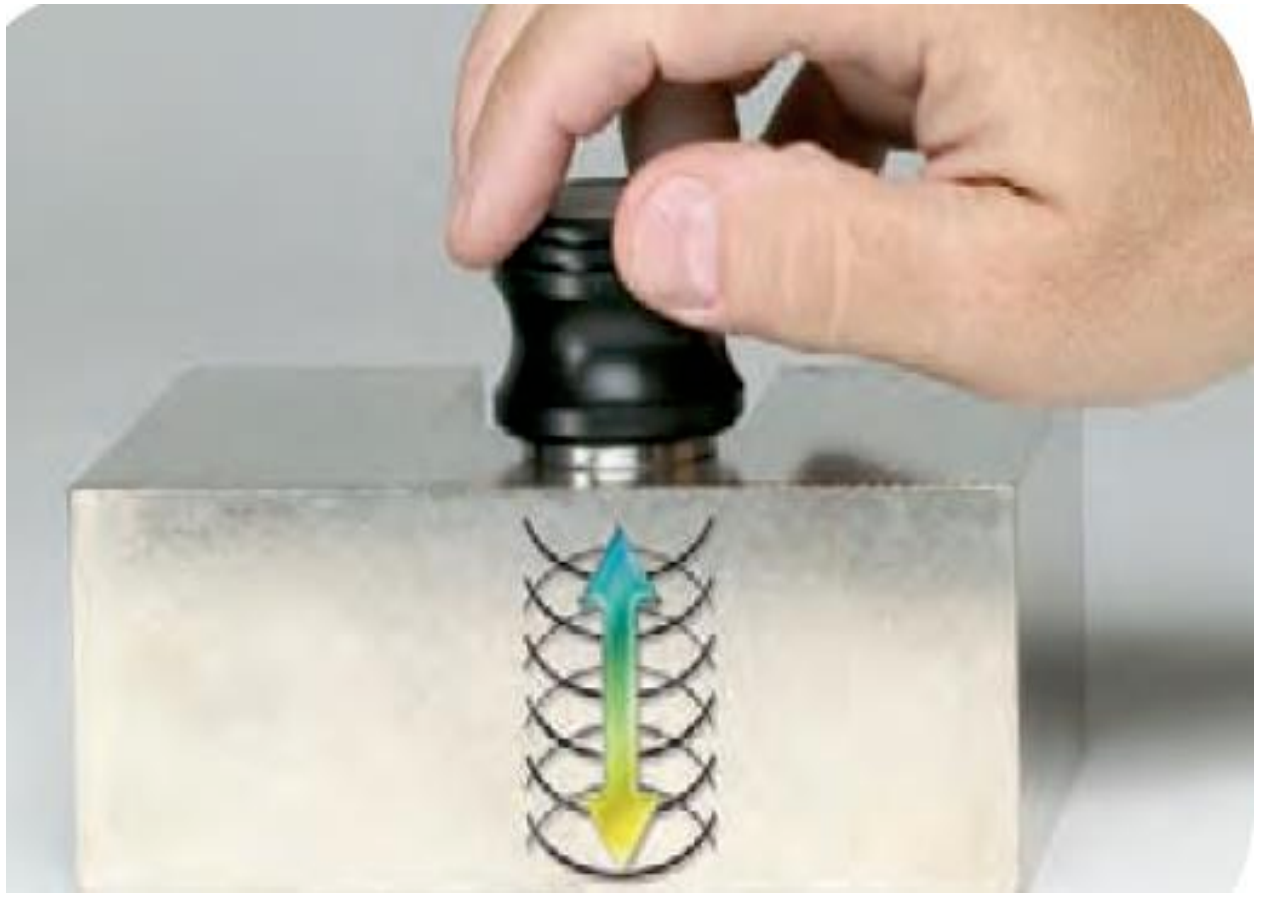
\includegraphics[width=\linewidth]{p03_img01.png}}\hfill
\subcaptionbox{测试信号}[0.47\textwidth]{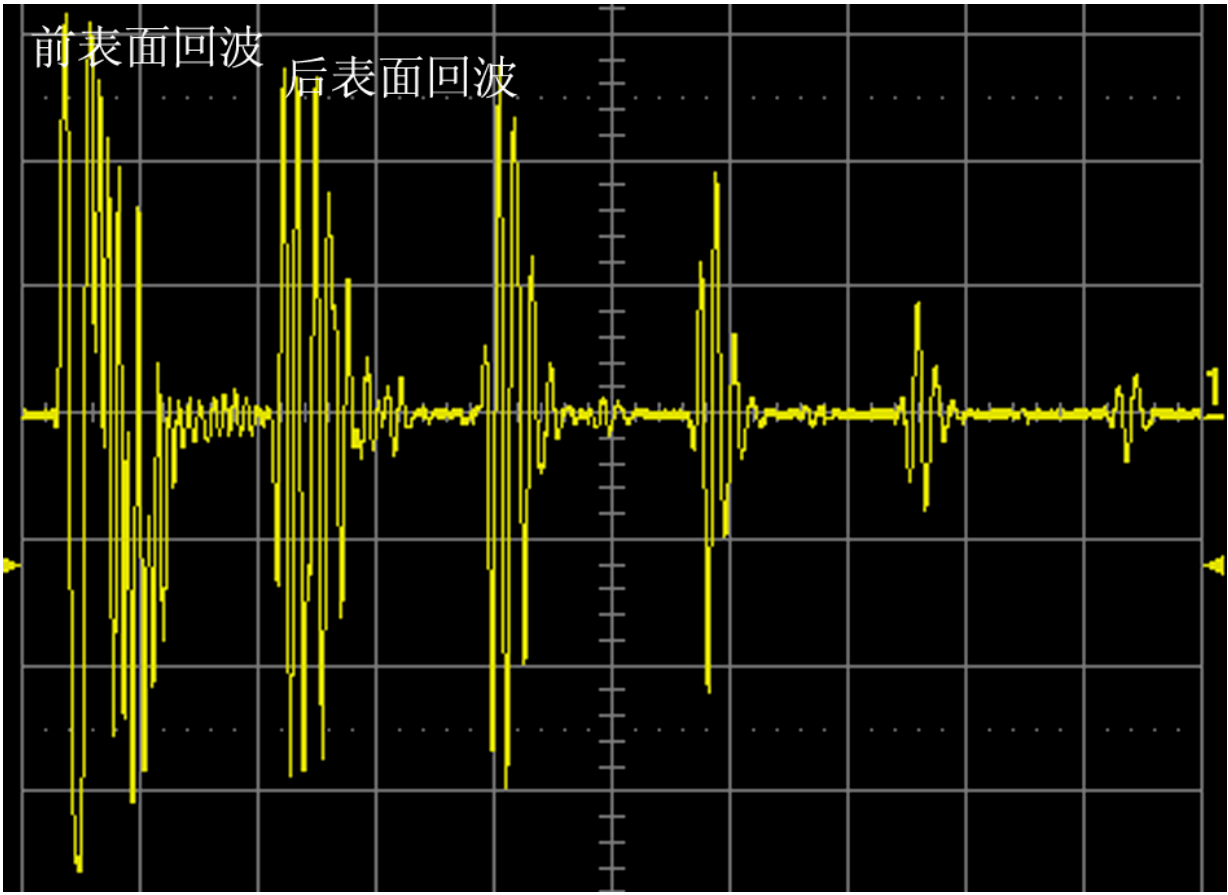
\includegraphics[width=\linewidth]{p03_img02.png}}
\caption{脉冲--回波方法}
\label{fig:exp2-pulse-echo}
\end{figure}

\subsubsection{波速}
根据回波信号得到两个回波峰值之间的时间差 $\Delta t$，并已知超声波传播路程 $\Delta L$ 为试件厚度 $d$ 的两倍，可计算出超声波的传播速度
\begin{equation}
  C=\frac{2d}{\Delta t}.
  \label{eq:exp2-speed}
\end{equation}

\subsubsection{衰减系数}
在介质中传播的超声平面波，其声压和声强振幅随传播距离 $x$ 的增加呈指数衰减，即
\begin{subequations}
\begin{align}
  P_x&=P_0e^{-\alpha x},\\
  I_x&=I_0e^{-2\alpha x}.
\end{align}
\end{subequations}
其中 $P$ 为声压，$I$ 为声强，$x$ 为声波传播的距离，$\alpha$ 为材料的衰减系数（单位为 NP/cm）。根据多次反射的回波信号，可以计算材料的衰减系数。对于任意两个回波 $n,m$（$n>m$），通过其峰值之间的幅值比可得到
\begin{equation}
  \alpha=\frac{1}{2(n-m)d}\ln\frac{P_m}{P_n}\quad(\mathrm{NP/cm}).
\end{equation}
实际测量中常采用 dB/cm 为单位，则衰减系数为
\begin{equation}
  \alpha=\frac{20}{2(n-m)d}\log_{10}\frac{|P_m|}{|P_n|}\quad(\mathrm{dB/cm}).
  \label{eq:exp2-attenuation}
\end{equation}
两种单位之间的换算关系为 $1\,\mathrm{NP/cm}=8.69\,\mathrm{dB/cm}$。

\subsubsection{材料常数（弹性模量和泊松比）}
根据无限弹性固体介质中波的传播特性，可得
\begin{subequations}
\begin{align}
  C_L&=\sqrt{\frac{E(1-\nu)}{\rho(1+\nu)(1-2\nu)}},\\
  C_S&=\sqrt{\frac{E}{2\rho(1+\nu)}}=\sqrt{\frac{G}{\rho}}.
\end{align}
\end{subequations}
通过测得材料中纵波和横波的波速 $C_L$ 和 $C_S$，即可得到材料的弹性模量和泊松比：
\begin{subequations}
\begin{align}
  \nu&=\frac{1-2(C_S/C_L)^2}{2-2(C_S/C_L)^2},\\
  E&=2\rho C_S^2(1+\nu).
  \label{eq:exp2-E}
\end{align}
\end{subequations}

\subsubsection{材料缺陷的检测}
如果知道试件厚度，可以通过测试波传播的时间差 $\Delta t$ 得到波速；反之，如果知道材料波速，可以通过测试前后表面波传播的时间差确定试件厚度，以及试件内部损伤的大小及位置。当超声波传播路径上无缺陷时，在探测信号入射波与底部回波之间不存在缺陷反射回波。当传播路径上存在缺陷，且缺陷界面小于探头晶片面积时，则同时存在缺陷反射回波和底面回波。当内部缺陷比较严重时，缺陷界面反射回波往往比较强，导致试件后表面无回波信号。因此，可以根据超声波反射回波特点对试件内部缺陷的位置及大小进行探测。

\begin{figure}[H]
  \centering
  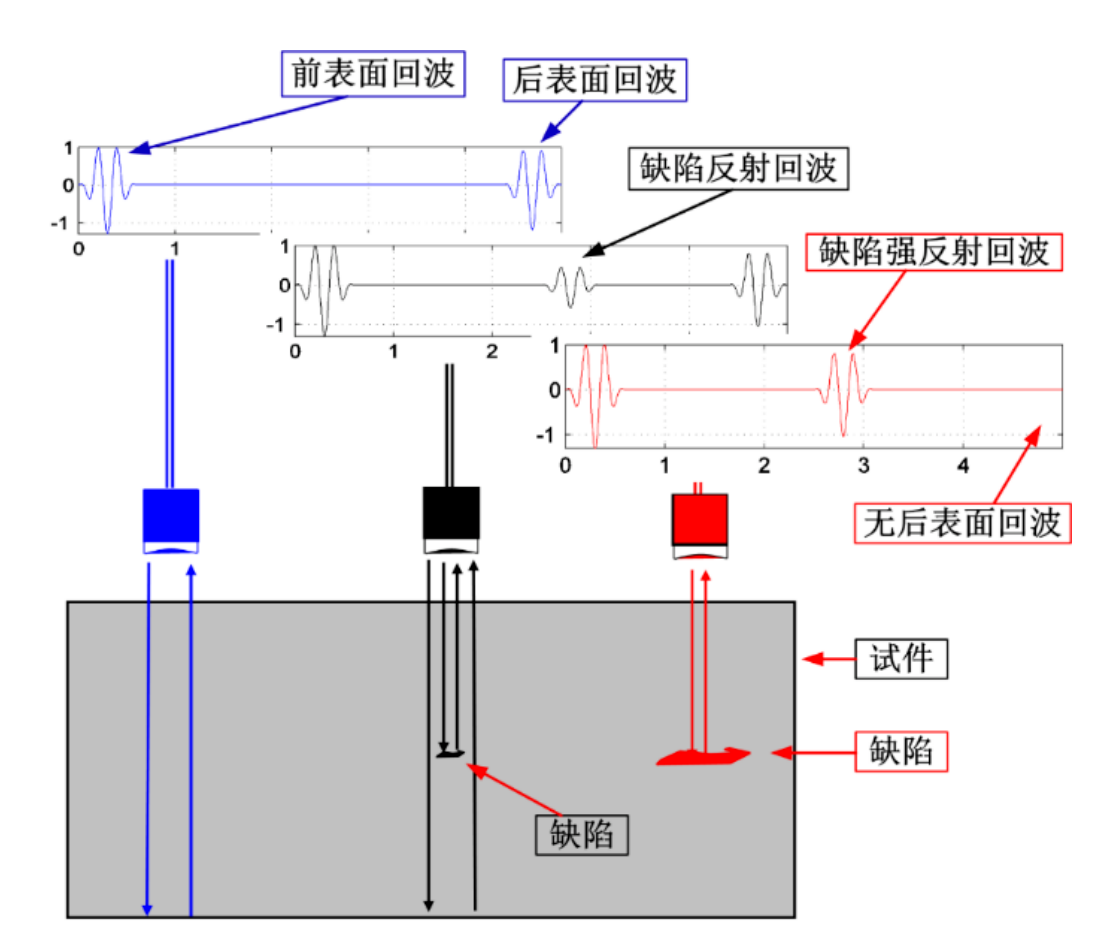
\includegraphics[width=0.5\textwidth]{p04_img01.png}
  \caption{有缺陷存在时波形示意图}
\end{figure}

超声波实验测试系统如图\ref{fig:exp2-system}所示。超声脉冲发射接收仪产生脉冲信号，通过超声探头转换为超声纵波或横波垂直入射到被测试件。同一探头接受试件底面反射的回波并转换为电信号，并采用数字存储示波器记录接收的信号进行分析。根据实验需要，可分别采用水浸式或接触式测试方式。超声纵波的测试两种方式都可以选择，只需选择对应探头；超声横波探头只能采用接触式测量。

\begin{figure}[H]
  \centering
  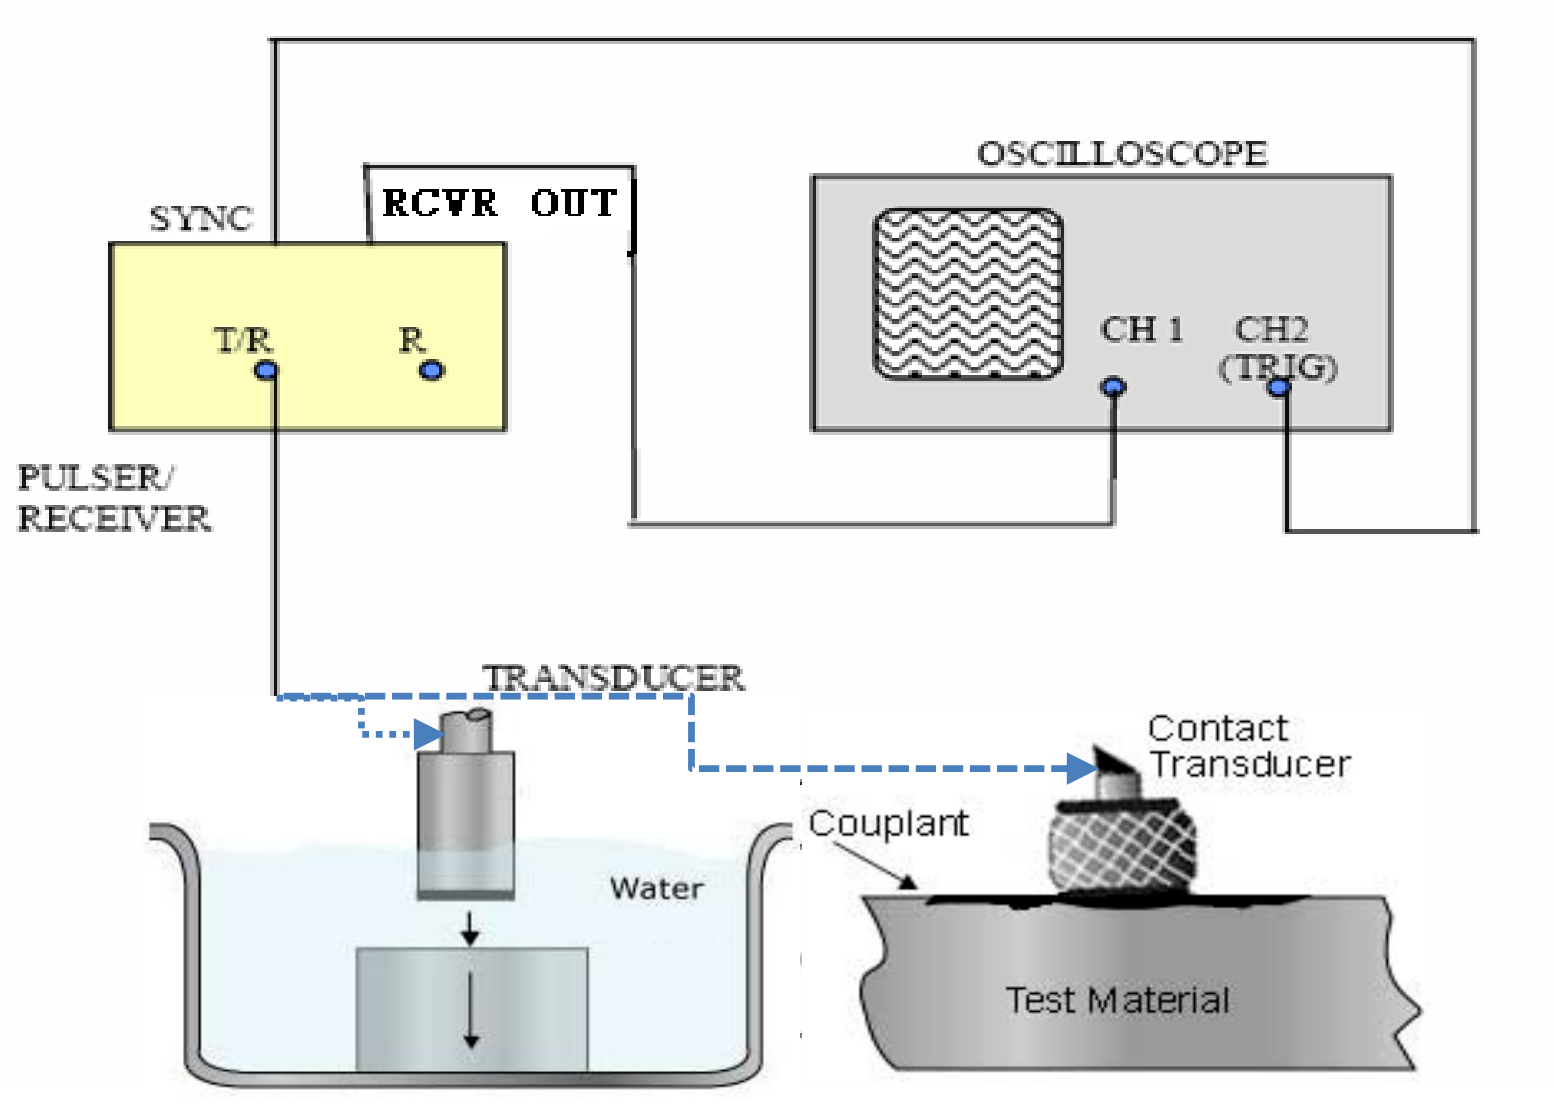
\includegraphics[width=0.7\textwidth]{p05_img01.png}
  \caption{实验测试系统示意图}
  \label{fig:exp2-system}
\end{figure}

\subsection{超声波实验测量的过程}
\subsubsection{材料密度测量}
多次测量试件的尺寸、质量，取其平均值，从而确定钢、铝和有机玻璃的密度。

\subsubsection{材料纵波波速和衰减系数测量}
\begin{enumerate}
  \item 实验准备：准备好装有足够水的水盆、酒精、脱脂棉等，并将水浸式超声探头架设在支架台上并探入水中。采用图\ref{fig:exp2-system}水浸式测量方式连接线路。
  \item 设置超声脉冲发射接收仪参数。
  \item 调节探头角度，使其垂直入射，测试超声波传播情况。测量探头距离盆底的距离，以便计算水的波速。
  \item 设置数字存储示波器参数，通过数字存储示波器采集超声探头接收的信号，并将数据及图像保存下来。
  \item 纵波波速测量：将钢、铝和有机玻璃分别放置于探头下，调整位置，进行测量。
  \item 数据分析：分析波形数据，得到所测材料的波速，并从多次反射峰值测超声波的衰减系数。
  \item 不同频率超声探头的纵波波速测量：采用纵波耦合剂接触式测量方式，分别采用 5 MHz 和 10 MHz 超声探头进行钢和有机玻璃的纵波波速测量。
  \item 不同频率超声探头的纵波衰减系数测量：采用纵波耦合剂接触式测量方式，分别采用 5 MHz 和 10 MHz 超声探头进行有机玻璃纵波衰减系数测量。
\end{enumerate}

\subsubsection{材料横波波速测量}
采用图\ref{fig:exp2-system}接触式测量方式连接线路，用酒精棉擦拭试件表面，将横波耦合剂涂于超声探头上，然后将横波超声探头与试件紧密接触，待信号稳定后采集并存储波形数据。所测试件分别为钢、铝和有机玻璃。

\subsubsection{钢板焊缝缺陷超声探测}
利用超声波脉冲回波模式，分别采用纵波超声直探头从钢板侧面垂直入射或斜探头从钢板表面斜入射的方式，对含焊缝钢板进行 B-Scan 超声探测，分析焊缝缺陷的位置及大小。
\begin{enumerate}
  \item 根据图\ref{fig:exp2-weld-setup}建立探测系统，选择探测模式，调节仪器参数。
  \item 在钢板侧面和表面画好探测路径并标好刻度，涂上纵波耦合剂。
  \item 在已画好的探测路径上每隔 0.5 cm 或 1 cm 进行一次超声探测，利用示波器和计算机进行信号数据采集存储。
  \item 通过分析所采集的信号，判断焊缝缺陷的位置和大小。
  \item 在钢板侧面纵波探测结果的基础上，在表面沿着与焊缝平行的方向，采用斜探头进行焊缝损伤的再次检测，并与前面的结果进行比较、分析。
\end{enumerate}

\begin{figure}[H]
  \centering
  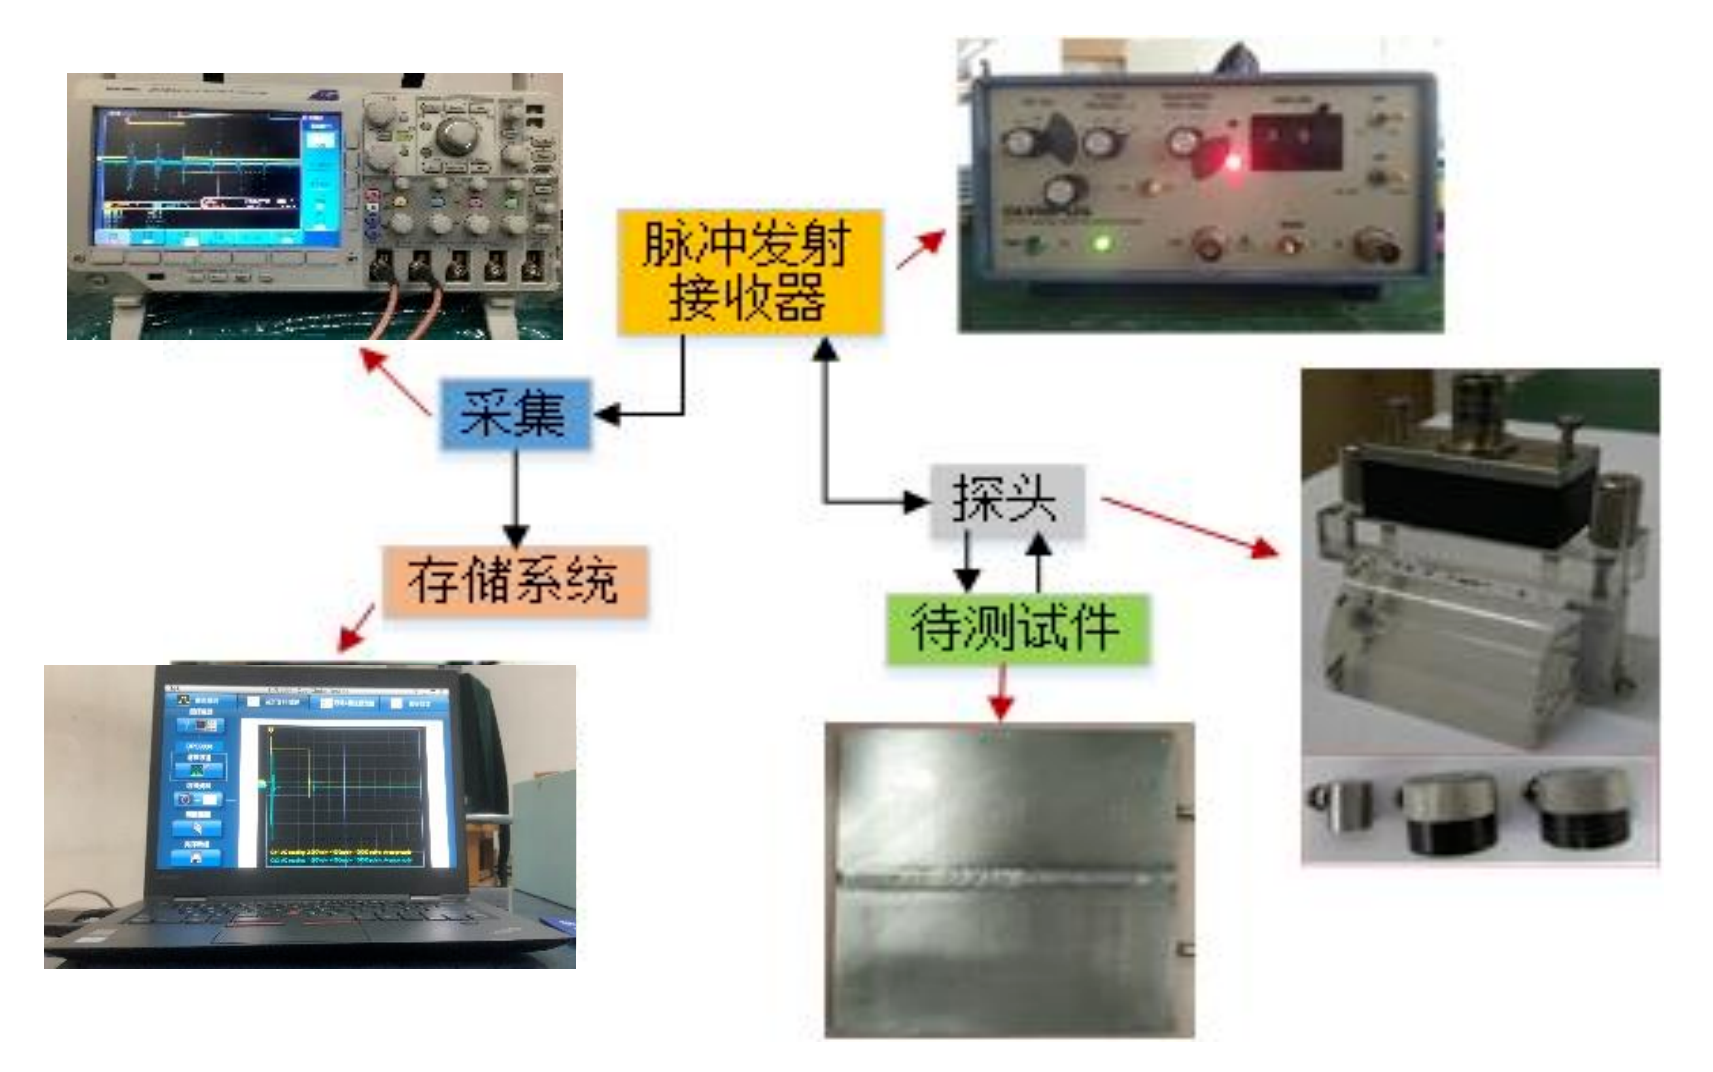
\includegraphics[width=0.75\textwidth]{p06_img01.png}
  \caption{钢板焊缝损伤检测}
  \label{fig:exp2-weld-setup}
\end{figure}

\section{脉冲--回波法测量波速和衰减系数、弹性模量和泊松比}
\noindent\textbf{使用说明：}以下实验结果图均从原报告提取，仅用于保留版式和读图示例。写作时请用同名文件替换为本组图像，并填写本组数据。

\subsection{材料密度测量}
分别多次测量材料质量 $m$ 和几何参数，所得结果填入表\ref{tab:exp2-density}。同时分析实验数据的不确定度。A 类不确定度的计算方法为
\begin{equation}
  u_A(X)=\sqrt{\frac{\sum_{i=1}^{n}(X_i-\bar{X})^2}{n(n-1)}}.
\end{equation}
B 类不确定度来自仪器误差：
\begin{equation}
  u_B(X)=\frac{\Delta}{\sqrt{3}}.
\end{equation}
合成不确定度为
\begin{equation}
  u(X)=\sqrt{u_A^2(X)+u_B^2(X)}.
\end{equation}

\begin{table}[H]
\centering\scriptsize
\caption{试件质量和尺寸测量结果}
\label{tab:exp2-density}
\setlength{\tabcolsep}{3pt}
\begin{tabular}{llccccccc}
\toprule
\multicolumn{2}{l}{测量对象} & 测量1 & 测量2 & 测量3 & 均值 & $u_A$ & $u_B$ & $u$\\
\midrule
\multirow{3}{*}{钢} & 质量（g） & \blank[0.7cm] & \blank[0.7cm] & \blank[0.7cm] & \blank[0.7cm] & \blank[0.7cm] & \blank[0.7cm] & \blank[0.7cm]\\
 & 直径（mm） & \blank[0.7cm] & \blank[0.7cm] & \blank[0.7cm] & \blank[0.7cm] & \blank[0.7cm] & \blank[0.7cm] & \blank[0.7cm]\\
 & 厚度（mm） & \blank[0.7cm] & \blank[0.7cm] & \blank[0.7cm] & \blank[0.7cm] & \blank[0.7cm] & \blank[0.7cm] & \blank[0.7cm]\\
\midrule
\multirow{3}{*}{铝} & 质量（g） & \blank[0.7cm] & \blank[0.7cm] & \blank[0.7cm] & \blank[0.7cm] & \blank[0.7cm] & \blank[0.7cm] & \blank[0.7cm]\\
 & 直径（mm） & \blank[0.7cm] & \blank[0.7cm] & \blank[0.7cm] & \blank[0.7cm] & \blank[0.7cm] & \blank[0.7cm] & \blank[0.7cm]\\
 & 厚度（mm） & \blank[0.7cm] & \blank[0.7cm] & \blank[0.7cm] & \blank[0.7cm] & \blank[0.7cm] & \blank[0.7cm] & \blank[0.7cm]\\
\midrule
\multirow{4}{*}{有机玻璃} & 质量（g） & \blank[0.7cm] & \blank[0.7cm] & \blank[0.7cm] & \blank[0.7cm] & \blank[0.7cm] & \blank[0.7cm] & \blank[0.7cm]\\
 & 长度（mm） & \blank[0.7cm] & \blank[0.7cm] & \blank[0.7cm] & \blank[0.7cm] & \blank[0.7cm] & \blank[0.7cm] & \blank[0.7cm]\\
 & 宽度（mm） & \blank[0.7cm] & \blank[0.7cm] & \blank[0.7cm] & \blank[0.7cm] & \blank[0.7cm] & \blank[0.7cm] & \blank[0.7cm]\\
 & 厚度（mm） & \blank[0.7cm] & \blank[0.7cm] & \blank[0.7cm] & \blank[0.7cm] & \blank[0.7cm] & \blank[0.7cm] & \blank[0.7cm]\\
\bottomrule
\end{tabular}
\end{table}

钢的平均密度及不确定度为
\begin{align}
  \bar{\rho}_{st}&=\frac{4\bar{m}_{st}}{\pi\bar{d}_{st}^{\,2}\bar{h}_{st}}
  =\blank[1.8cm]\ \mathrm{g/cm^3},\\
  u(\rho_{st})&=\bar{\rho}_{st}\sqrt{
  \left[\frac{u(m_{st})}{\bar{m}_{st}}\right]^2+
  \left[\frac{2u(d_{st})}{\bar{d}_{st}}\right]^2+
  \left[\frac{u(h_{st})}{\bar{h}_{st}}\right]^2}
  =\blank[1.5cm]\ \mathrm{g/cm^3},\\
  \rho_{st}&=\bar{\rho}_{st}\pm u(\rho_{st})
  =(\blank[1.2cm]\pm\blank[1.2cm])\ \mathrm{g/cm^3}.
\end{align}
铝的平均密度及不确定度为
\begin{align}
  \bar{\rho}_{al}&=\frac{4\bar{m}_{al}}{\pi\bar{d}_{al}^{\,2}\bar{h}_{al}}
  =\blank[1.8cm]\ \mathrm{g/cm^3},\\
  u(\rho_{al})&=\bar{\rho}_{al}\sqrt{
  \left[\frac{u(m_{al})}{\bar{m}_{al}}\right]^2+
  \left[\frac{2u(d_{al})}{\bar{d}_{al}}\right]^2+
  \left[\frac{u(h_{al})}{\bar{h}_{al}}\right]^2}
  =\blank[1.5cm]\ \mathrm{g/cm^3},\\
  \rho_{al}&=\bar{\rho}_{al}\pm u(\rho_{al})
  =(\blank[1.2cm]\pm\blank[1.2cm])\ \mathrm{g/cm^3}.
\end{align}
有机玻璃的平均密度及不确定度为
\begin{align}
  \bar{\rho}_{og}&=\frac{\bar{m}_{og}}{\bar{a}_{og}\bar{b}_{og}\bar{h}_{og}}
  =\blank[1.8cm]\ \mathrm{g/cm^3},\\
  u(\rho_{og})&=\bar{\rho}_{og}\sqrt{
  \left[\frac{u(m_{og})}{\bar{m}_{og}}\right]^2+
  \left[\frac{u(a_{og})}{\bar{a}_{og}}\right]^2+
  \left[\frac{u(b_{og})}{\bar{b}_{og}}\right]^2+
  \left[\frac{u(h_{og})}{\bar{h}_{og}}\right]^2}
  =\blank[1.5cm]\ \mathrm{g/cm^3},\\
  \rho_{og}&=\bar{\rho}_{og}\pm u(\rho_{og})
  =(\blank[1.2cm]\pm\blank[1.2cm])\ \mathrm{g/cm^3}.
\end{align}

\subsection{水的纵波波速}
将频率为 5 MHz 的水浸式超声探头浸入水中并调整角度，使探头垂直入射。选用合适大小的试件固定探头和盆底的距离，之后取出试件并测量其厚度，即为探头与底部的距离 $h$。根据示波器波形测量入射波与反射波之间的时间差 $\Delta t$，即可由式\eqref{eq:exp2-speed}计算水中波速。$h$ 的测量数据填入表\ref{tab:exp2-water-distance}，信号图如图\ref{fig:exp2-water-signal}所示。

\begin{table}[H]
\centering\small
\caption{测量水中纵波波速时探头与水池底部距离}
\label{tab:exp2-water-distance}
\begin{tabular}{lccccccc}
\toprule
测量对象 & 测量1 & 测量2 & 测量3 & 均值 & $u_A$ & $u_B$ & $u$\\
\midrule
距离（mm） & \blank[1cm] & \blank[1cm] & \blank[1cm] & \blank[1cm] & \blank[0.8cm] & \blank[0.8cm] & \blank[0.8cm]\\
\bottomrule
\end{tabular}
\end{table}

\begin{figure}[H]
\centering
\subcaptionbox{输入输出信号全局图}[0.48\textwidth]{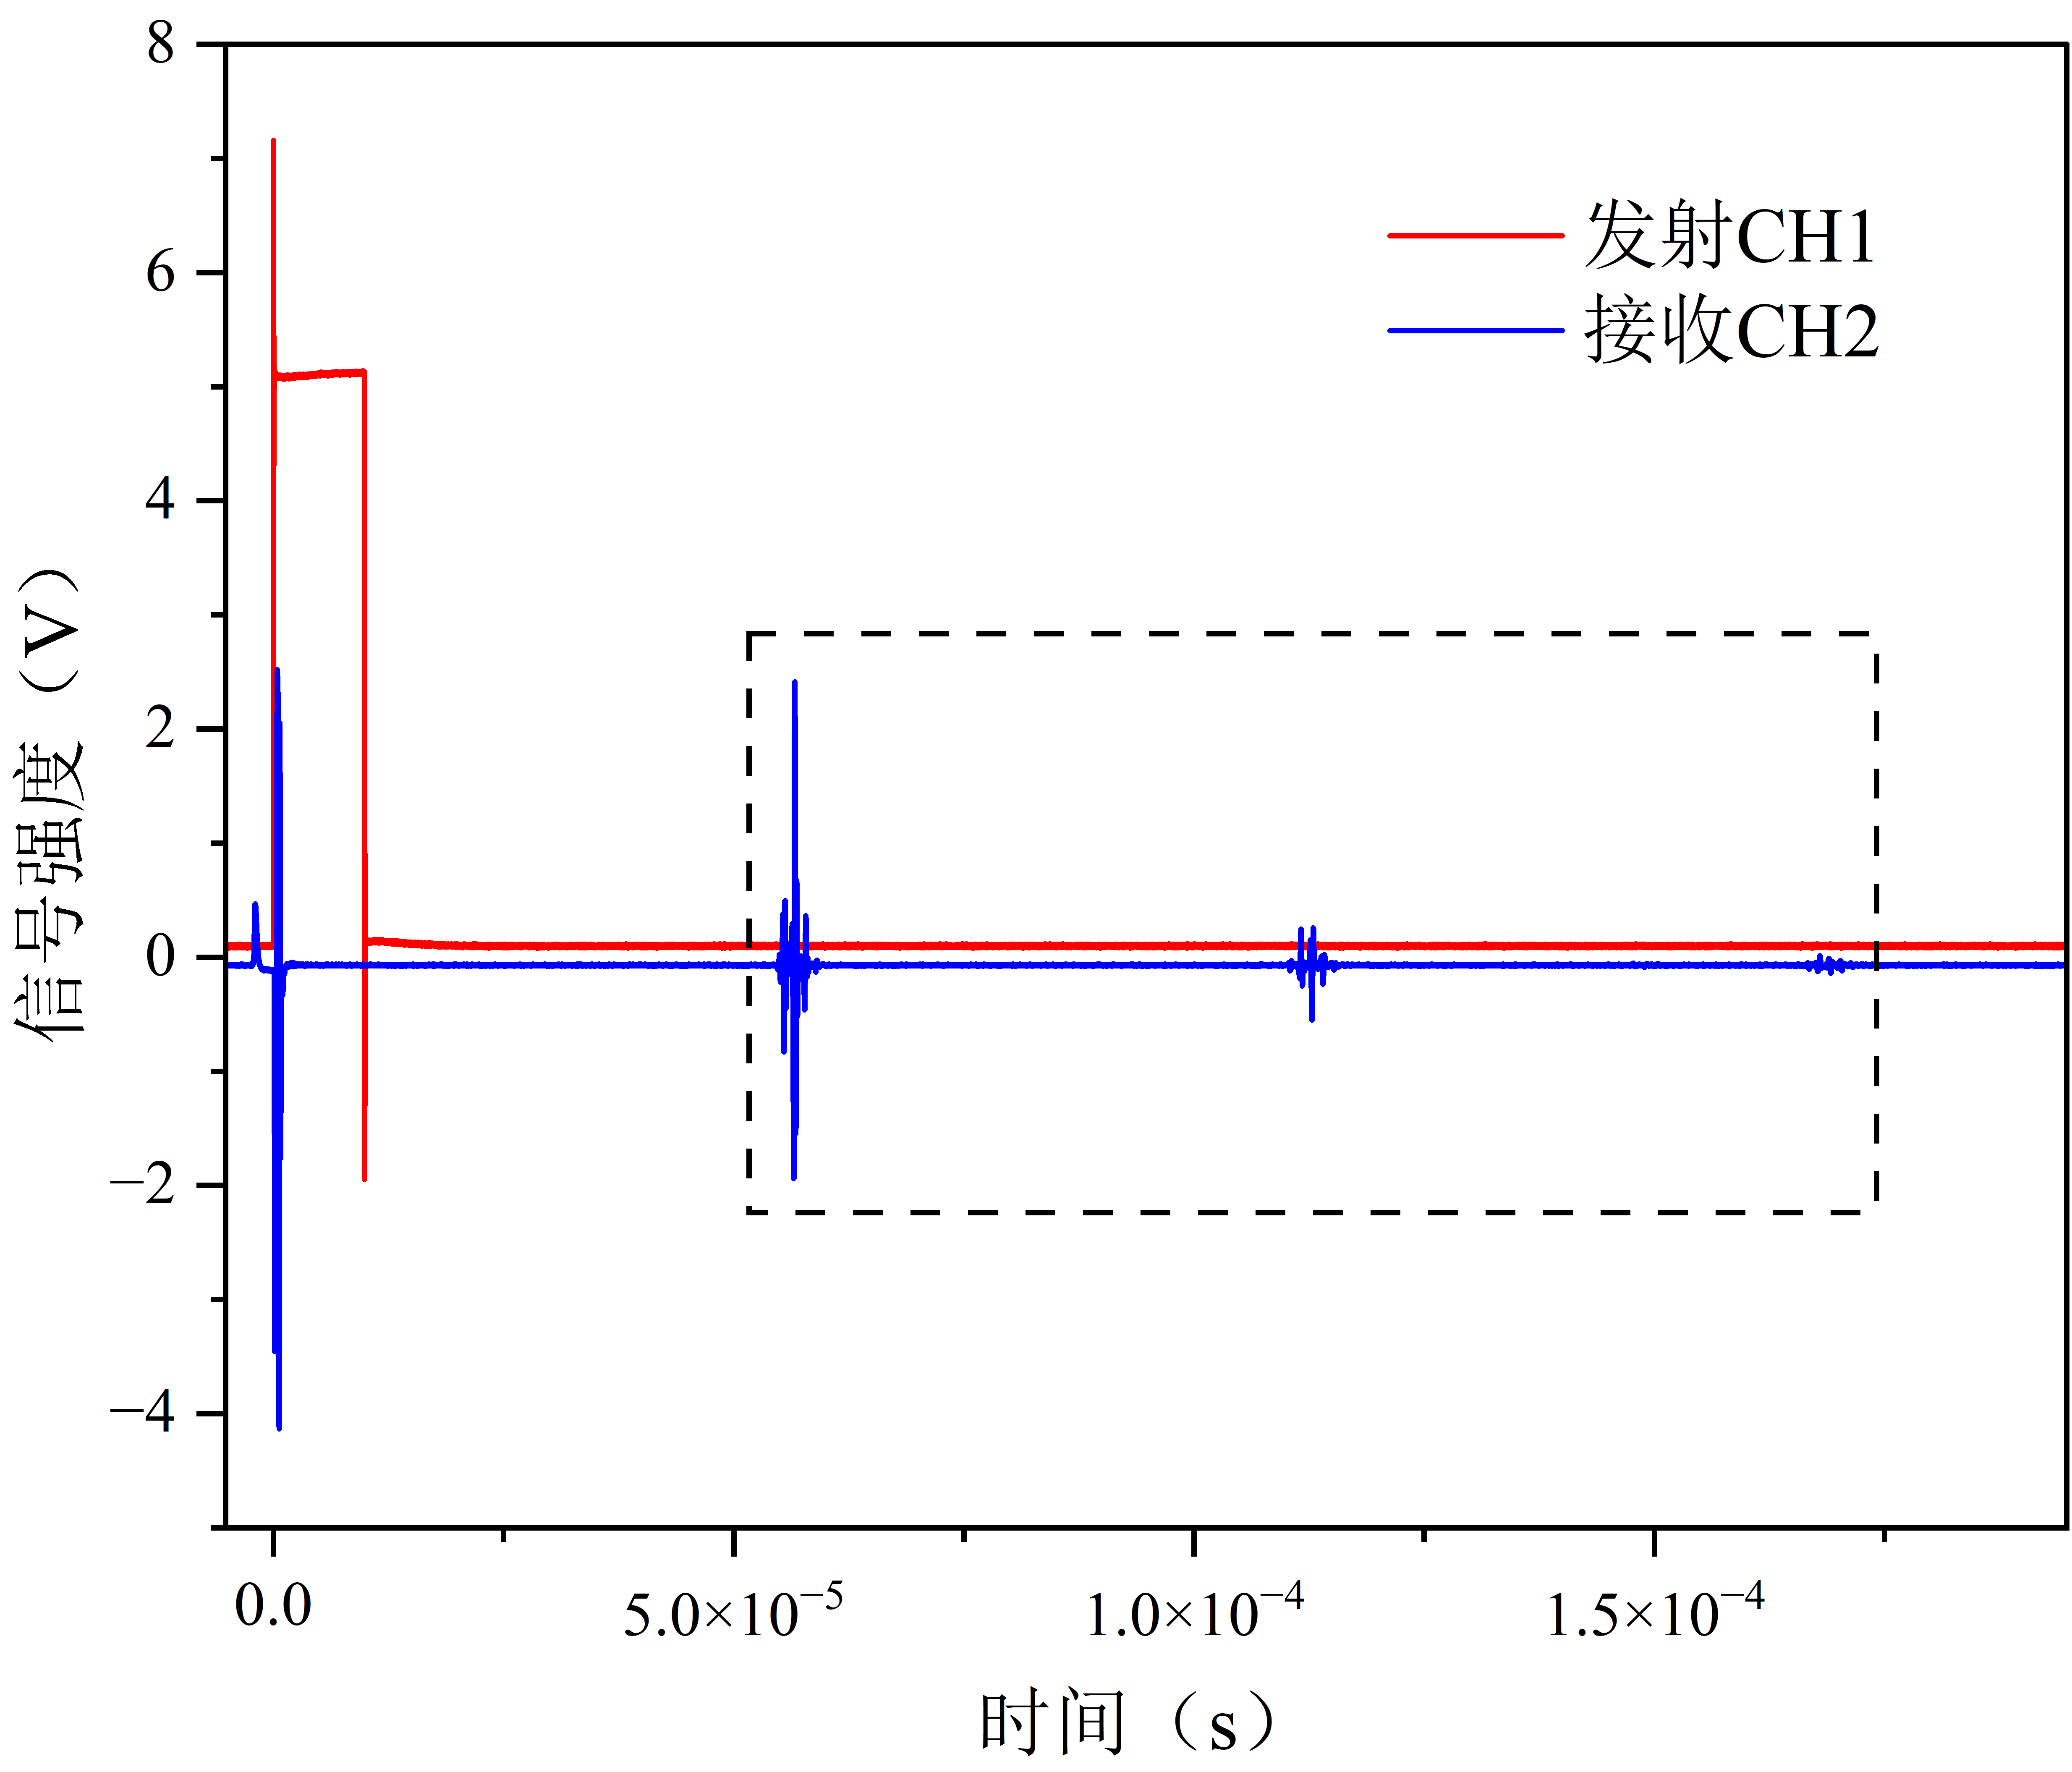
\includegraphics[width=\linewidth]{p08_img01.png}}\hfill
\subcaptionbox{输出信号局部放大图}[0.48\textwidth]{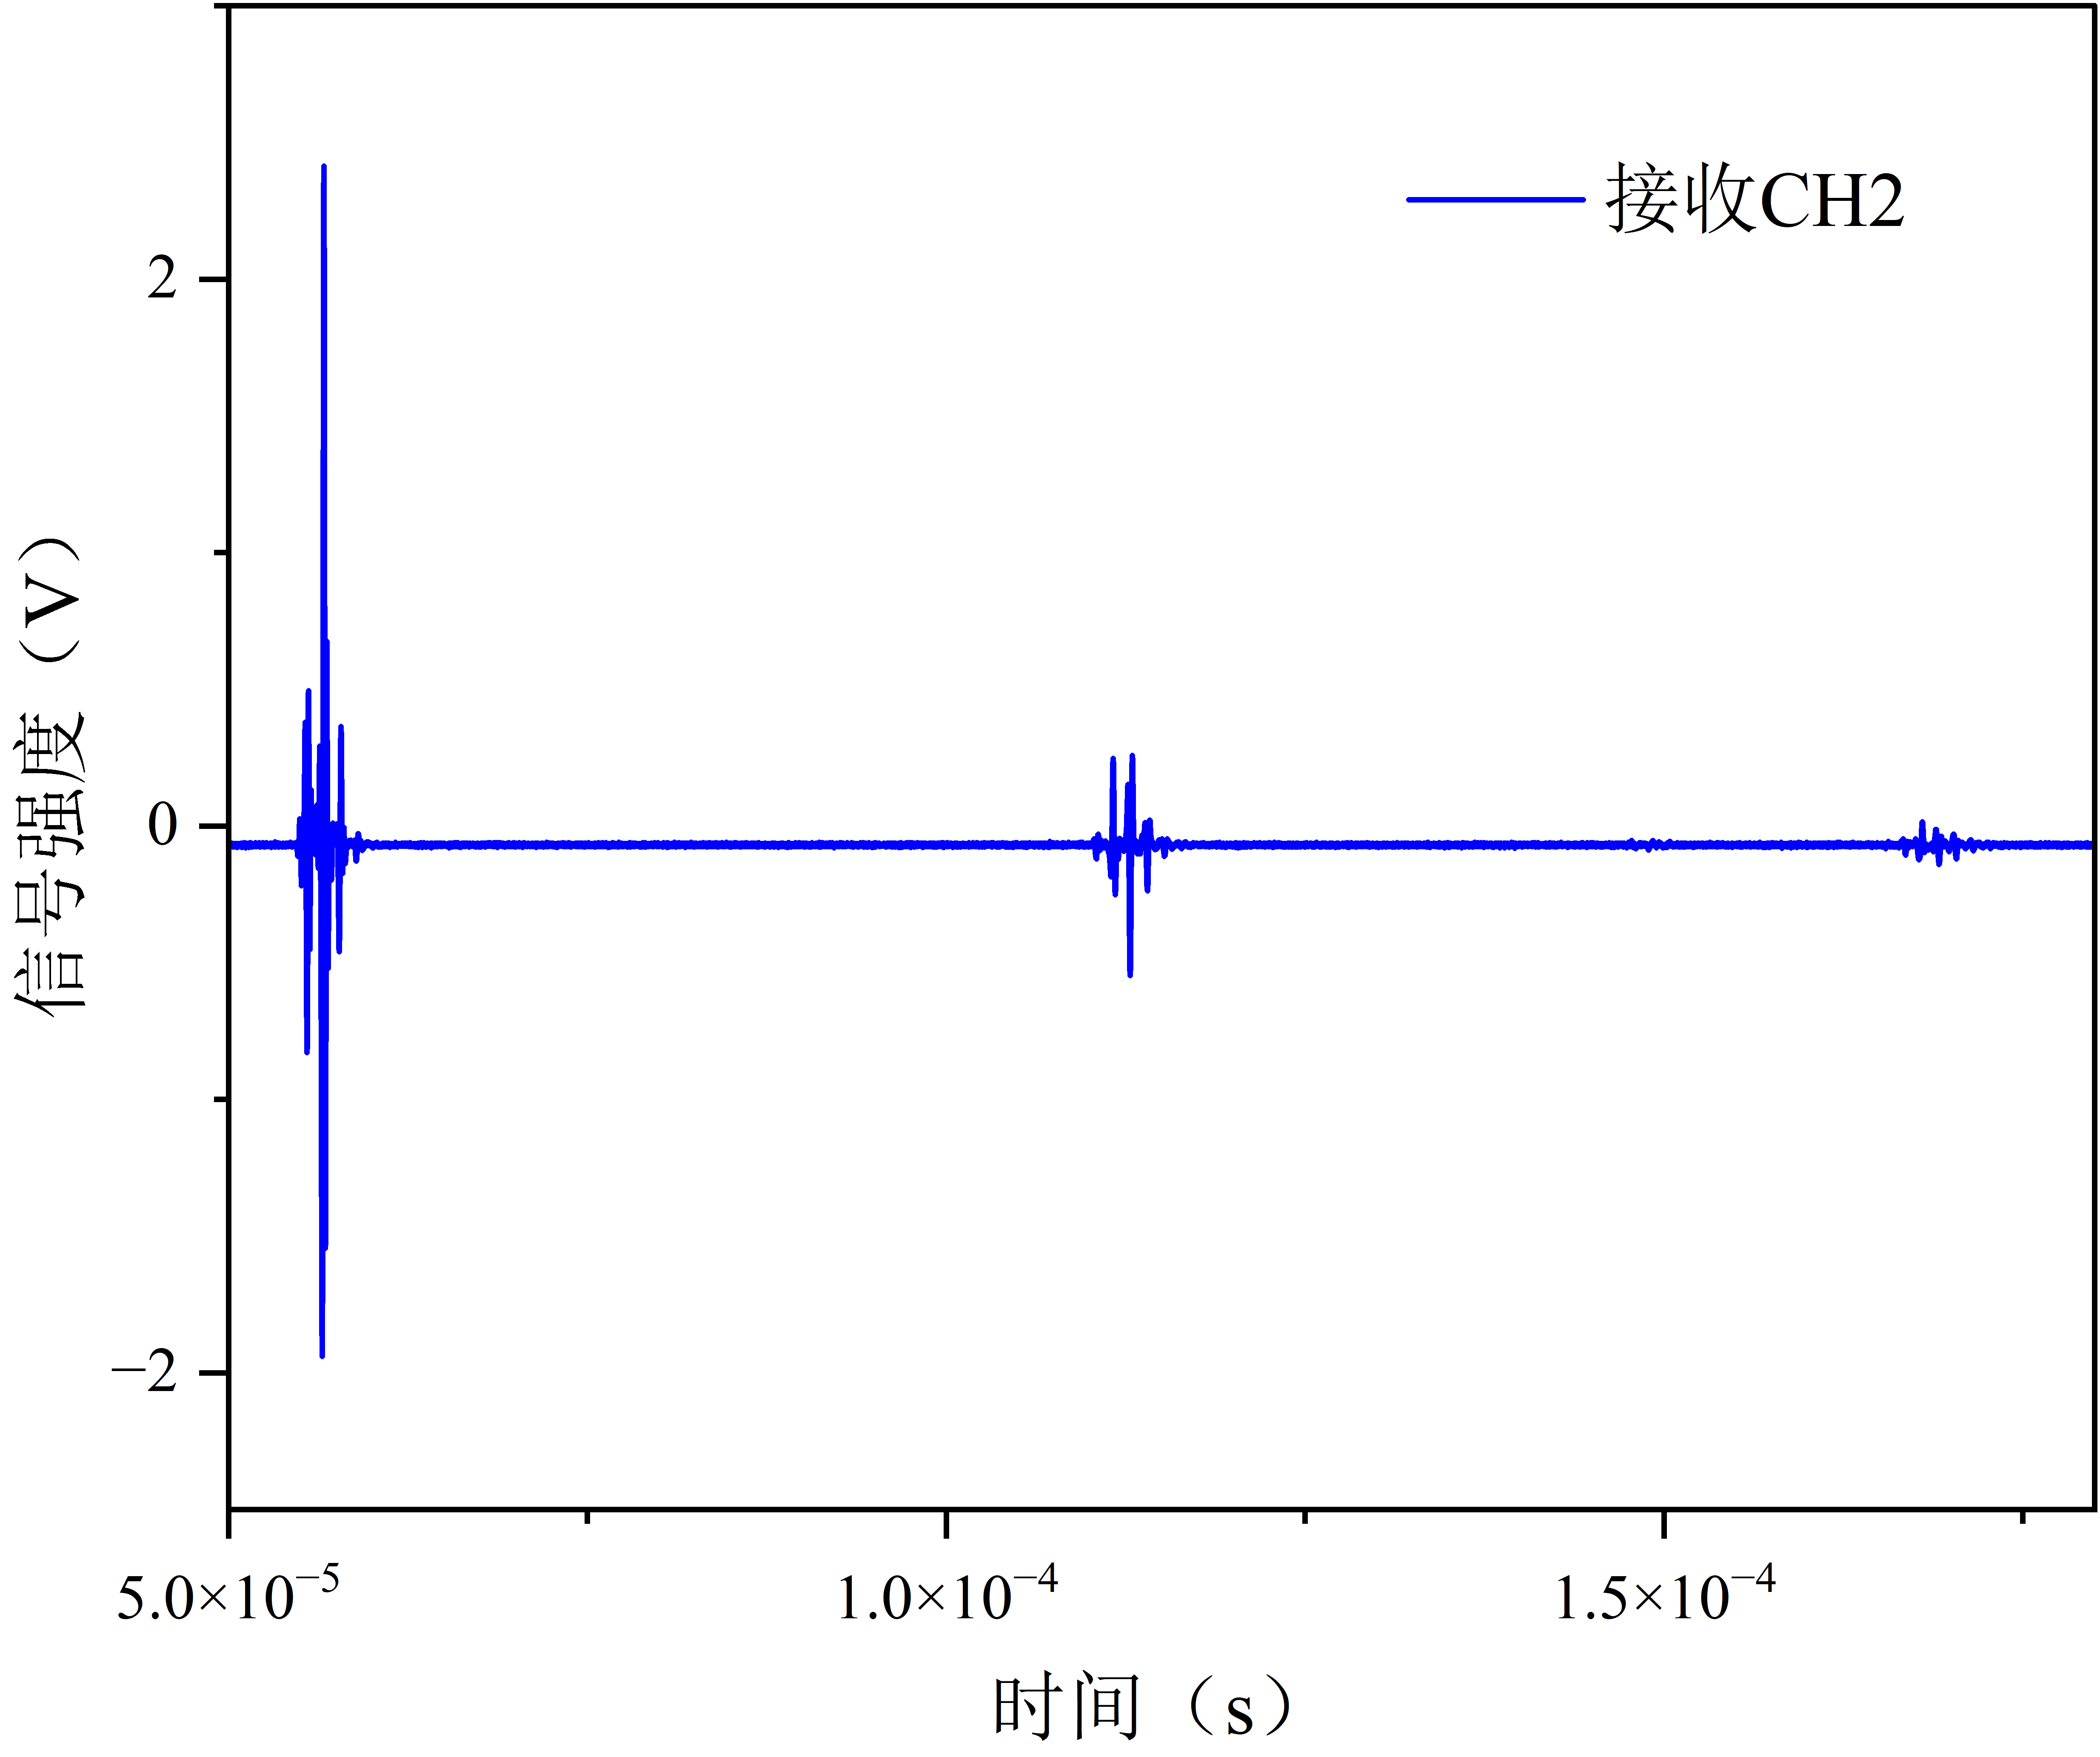
\includegraphics[width=\linewidth]{p08_img02.png}}
\caption{5 MHz 测量水中纵波波速时信号图（请替换为本组图像）}
\label{fig:exp2-water-signal}
\end{figure}

\begin{table}[H]
\centering\small
\caption{5 MHz 测量水中纵波波速时波峰之间的时间差}
\label{tab:exp2-water-time}
\begin{tabular}{lcccccc}
\toprule
测量对象 & 测量1 & 测量2 & 均值 & $u_A$ & $u_B$ & $u$\\
\midrule
$\Delta t$（$\mu$s） & \blank[1.2cm] & \blank[1.2cm] & \blank[1.2cm] & \blank[1cm] & \blank[0.8cm] & \blank[1cm]\\
\bottomrule
\end{tabular}
\end{table}

水中纵波的平均波速、不确定度与测量结果为
\begin{align}
  \bar{C}_{water}&=\frac{2\bar{h}}{\overline{\Delta t}}
  =\blank[2cm]\ \mathrm{m/s},\\
  u(C_{water})&=\bar{C}_{water}\sqrt{
  \left[\frac{u(h)}{\bar{h}}\right]^2+
  \left[\frac{u(\Delta t)}{\overline{\Delta t}}\right]^2}
  =\blank[1.8cm]\ \mathrm{m/s},\\
  C_{water}&=\bar{C}_{water}\pm u(C_{water})
  =(\blank[1.5cm]\pm\blank[1.5cm])\ \mathrm{m/s}.
\end{align}
常温水中的超声波波速参考值取 $C=1480\,\mathrm{m/s}$，相对误差为
\begin{equation}
  \Delta=\frac{|C_{water}-C|}{C}\times100\%=\blank[2cm].
\end{equation}
分析距离测量、探头移动及读数等因素对结果的影响。
\answer

\subsection{水浸式测量三种材料的纵波波速}
利用频率为 5 MHz 的水浸式超声探头测量纵波在钢、铝、有机玻璃中的传播速度。将试件依次放入水中，调整探头方向使其垂直于试件表面，待示波器信号稳定后记录并导出数据。波形及用于计算波速的数据区域如图\ref{fig:exp2-steel-L}--图\ref{fig:exp2-og-L}所示，波峰时间差填入表\ref{tab:exp2-L-time}。

\begin{figure}[H]
\centering
\subcaptionbox{输入输出信号全局图}[0.48\textwidth]{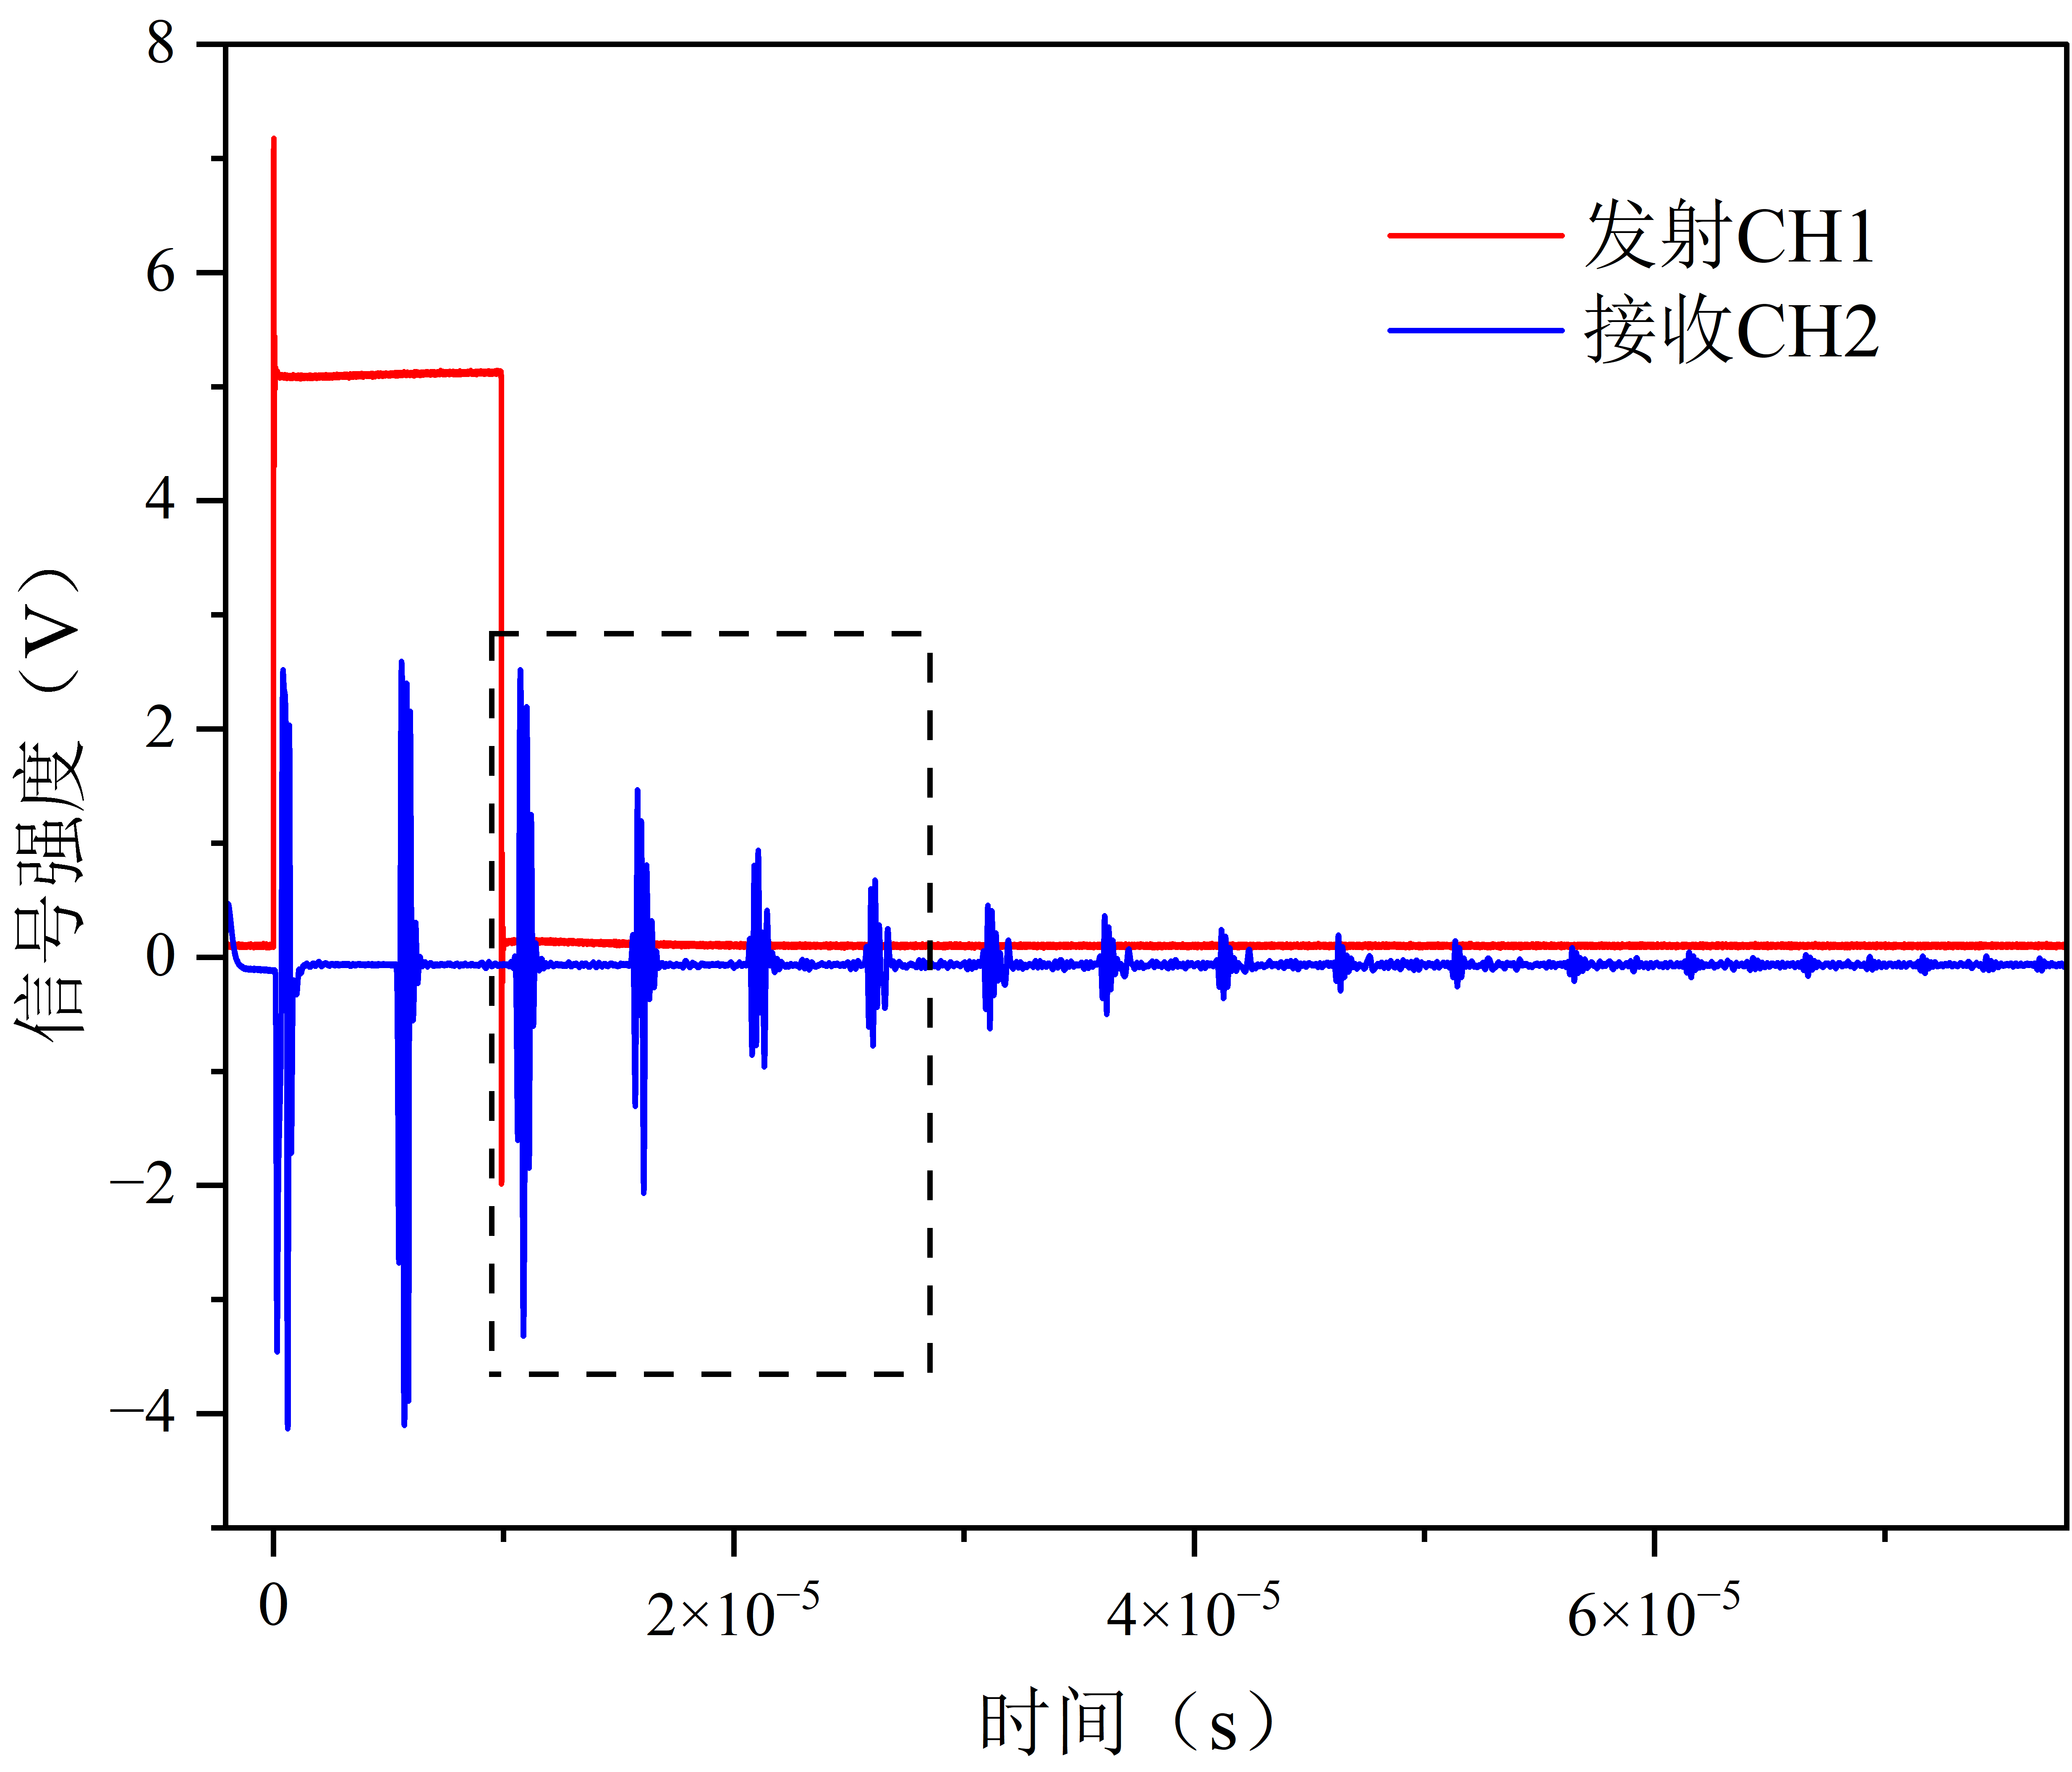
\includegraphics[width=\linewidth]{p09_img01.png}}\hfill
\subcaptionbox{输出信号局部放大图}[0.48\textwidth]{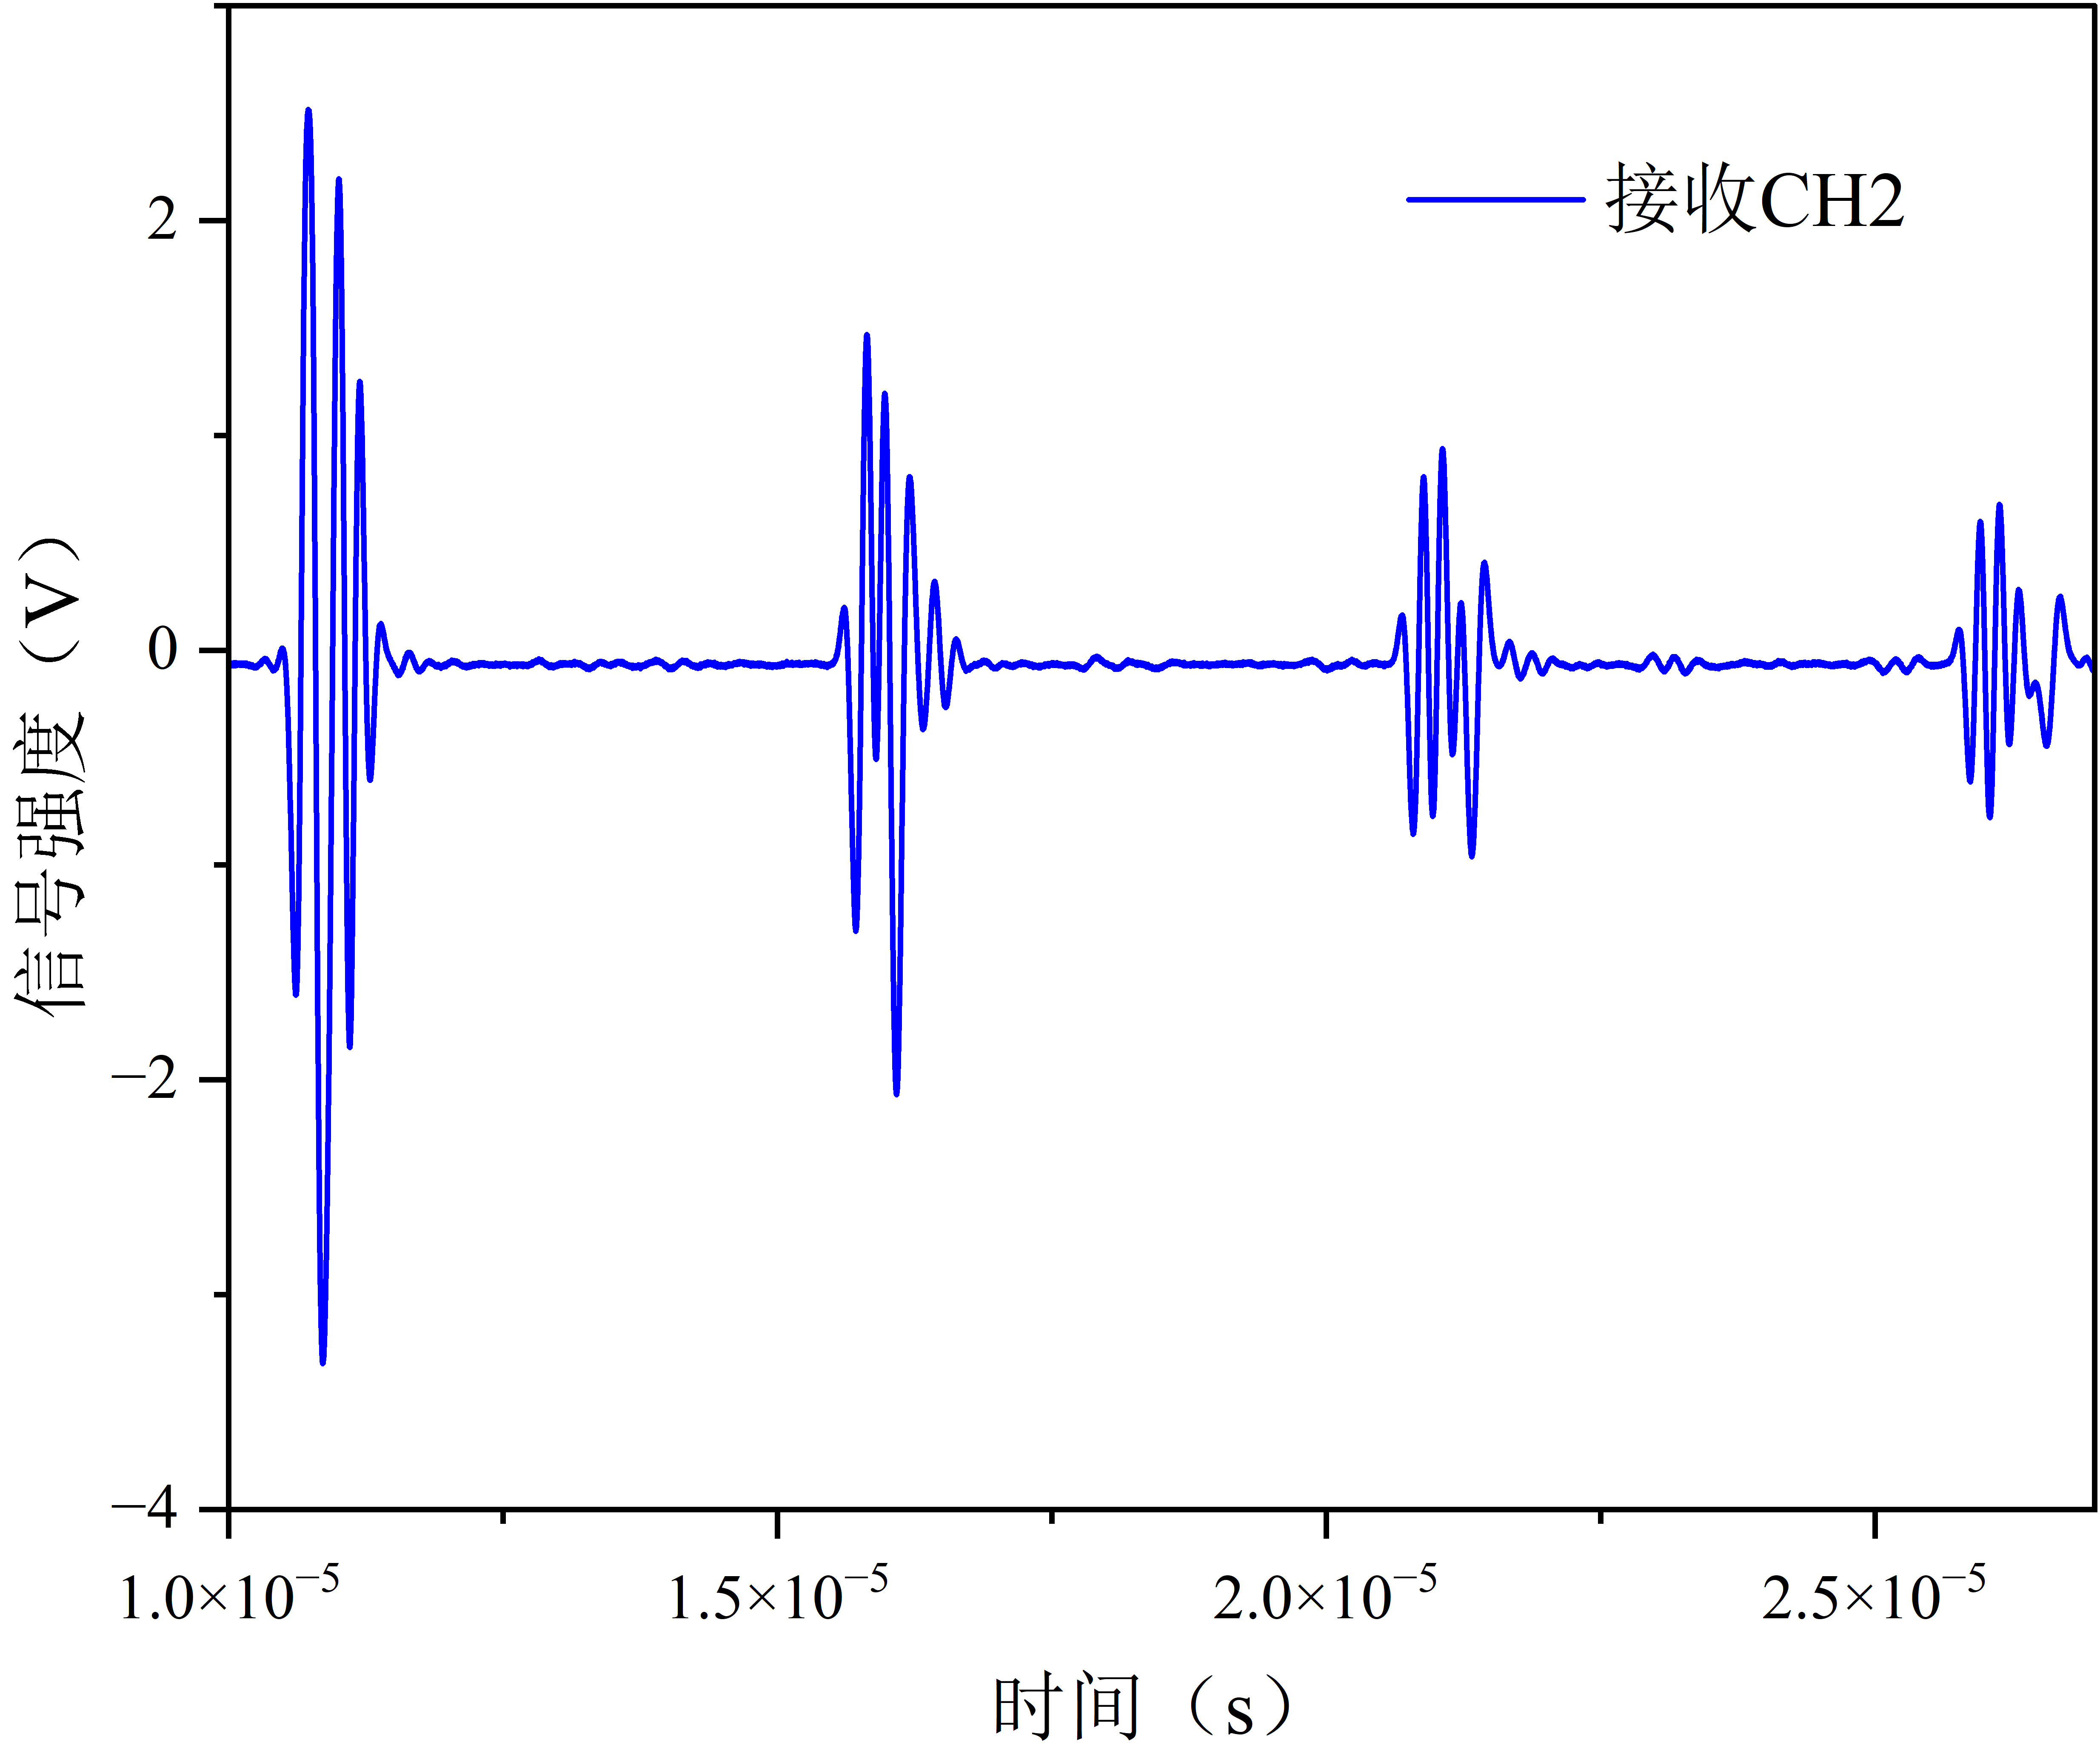
\includegraphics[width=\linewidth]{p09_img02.png}}
\caption{5 MHz 水浸式测量钢试件纵波波速时信号图}
\label{fig:exp2-steel-L}
\end{figure}

\begin{figure}[H]
\centering
\subcaptionbox{输入输出信号全局图}[0.48\textwidth]{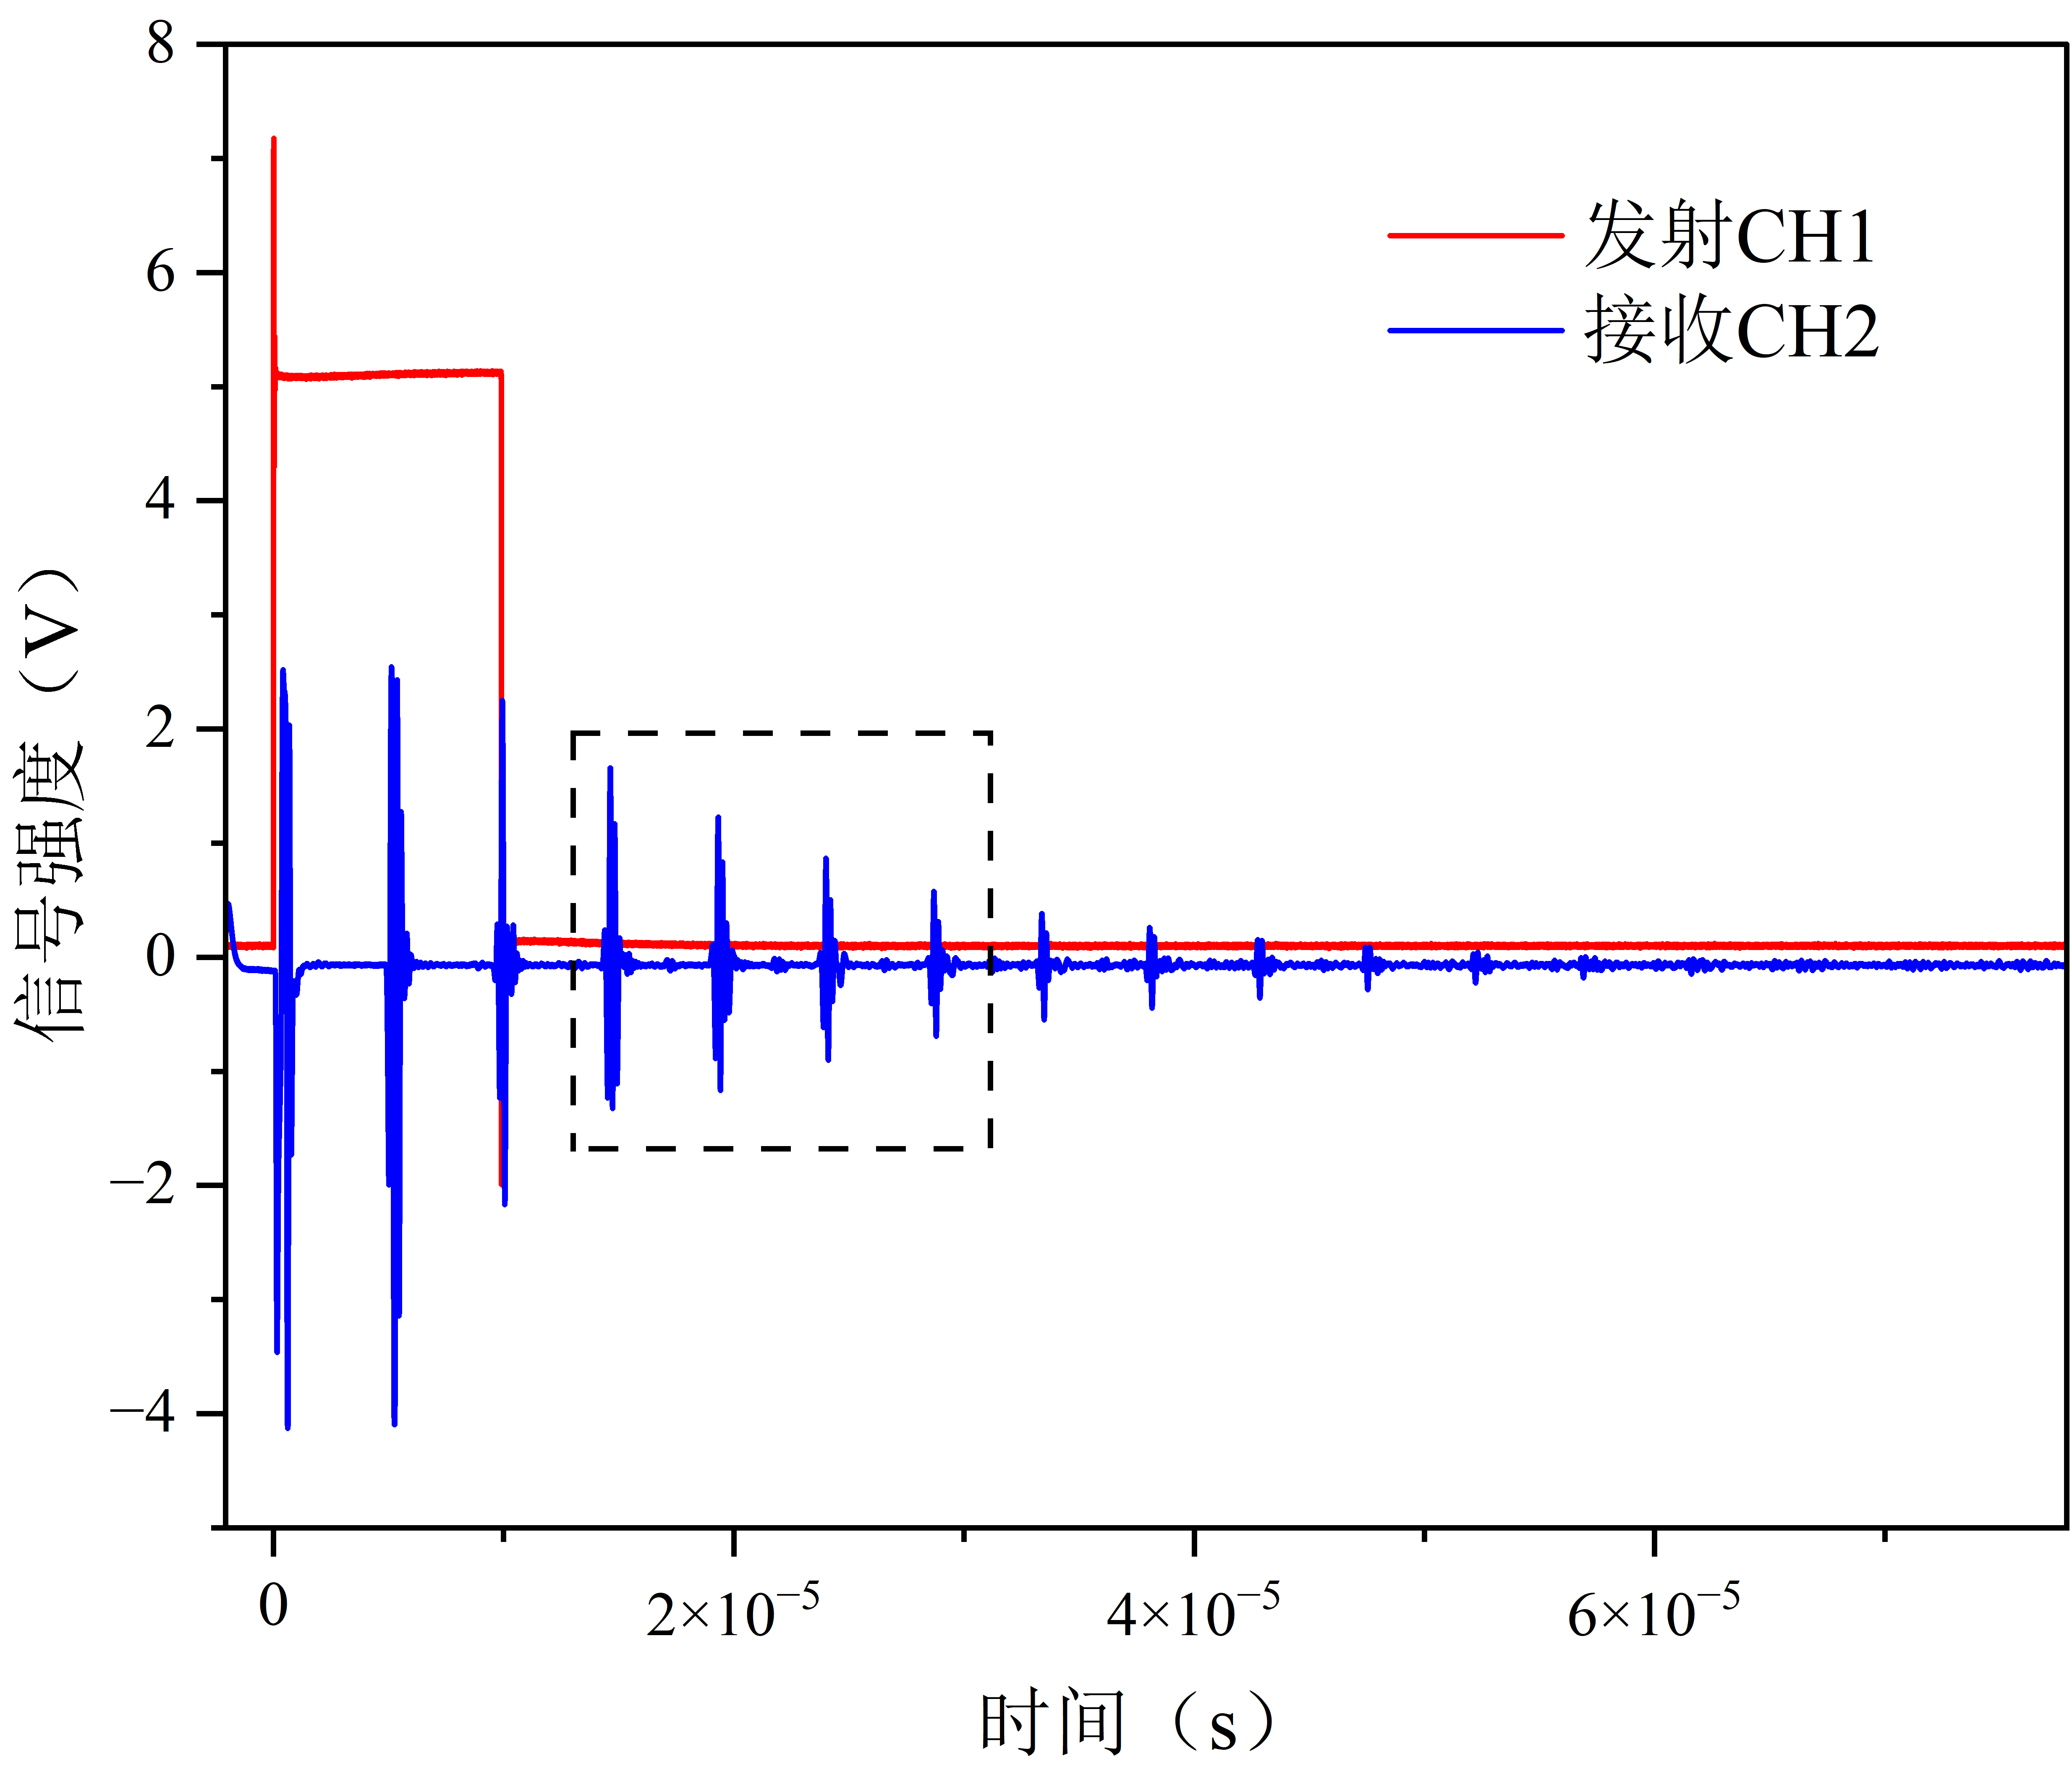
\includegraphics[width=\linewidth]{p09_img03.png}}\hfill
\subcaptionbox{输出信号局部放大图}[0.48\textwidth]{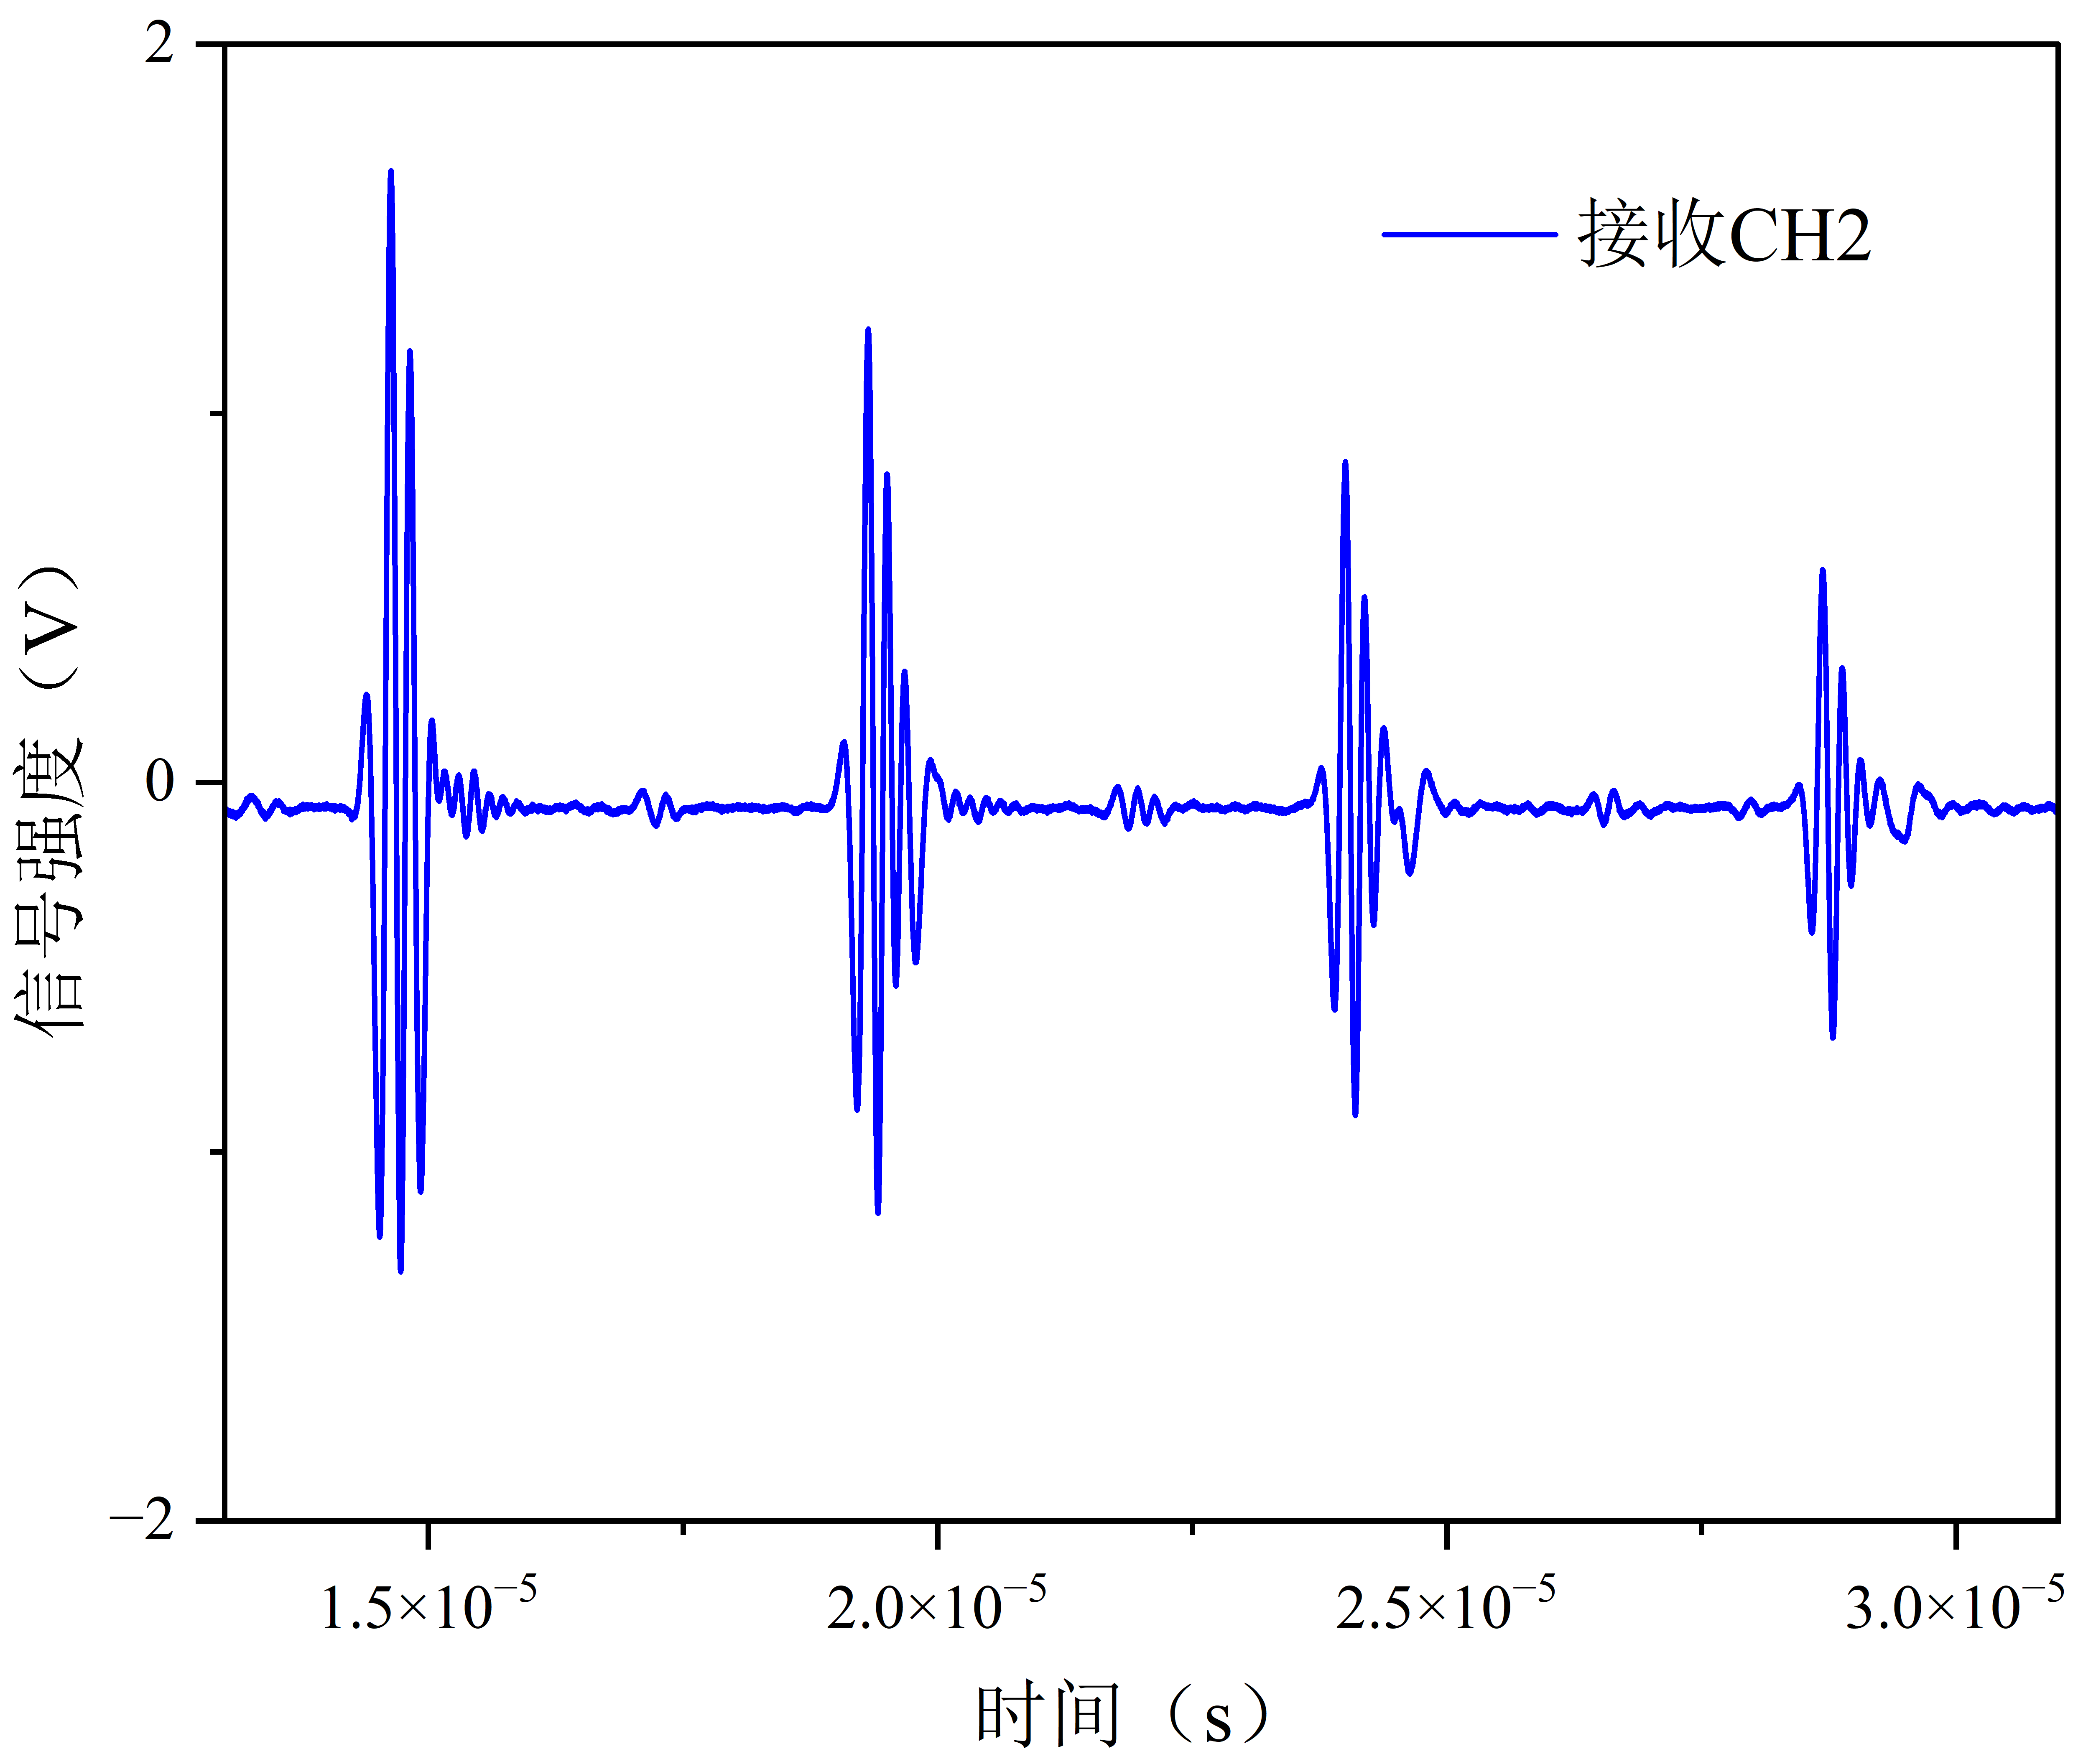
\includegraphics[width=\linewidth]{p09_img04.png}}
\caption{5 MHz 水浸式测量铝试件纵波波速时信号图}
\end{figure}

\begin{figure}[H]
\centering
\subcaptionbox{输入输出信号全局图}[0.48\textwidth]{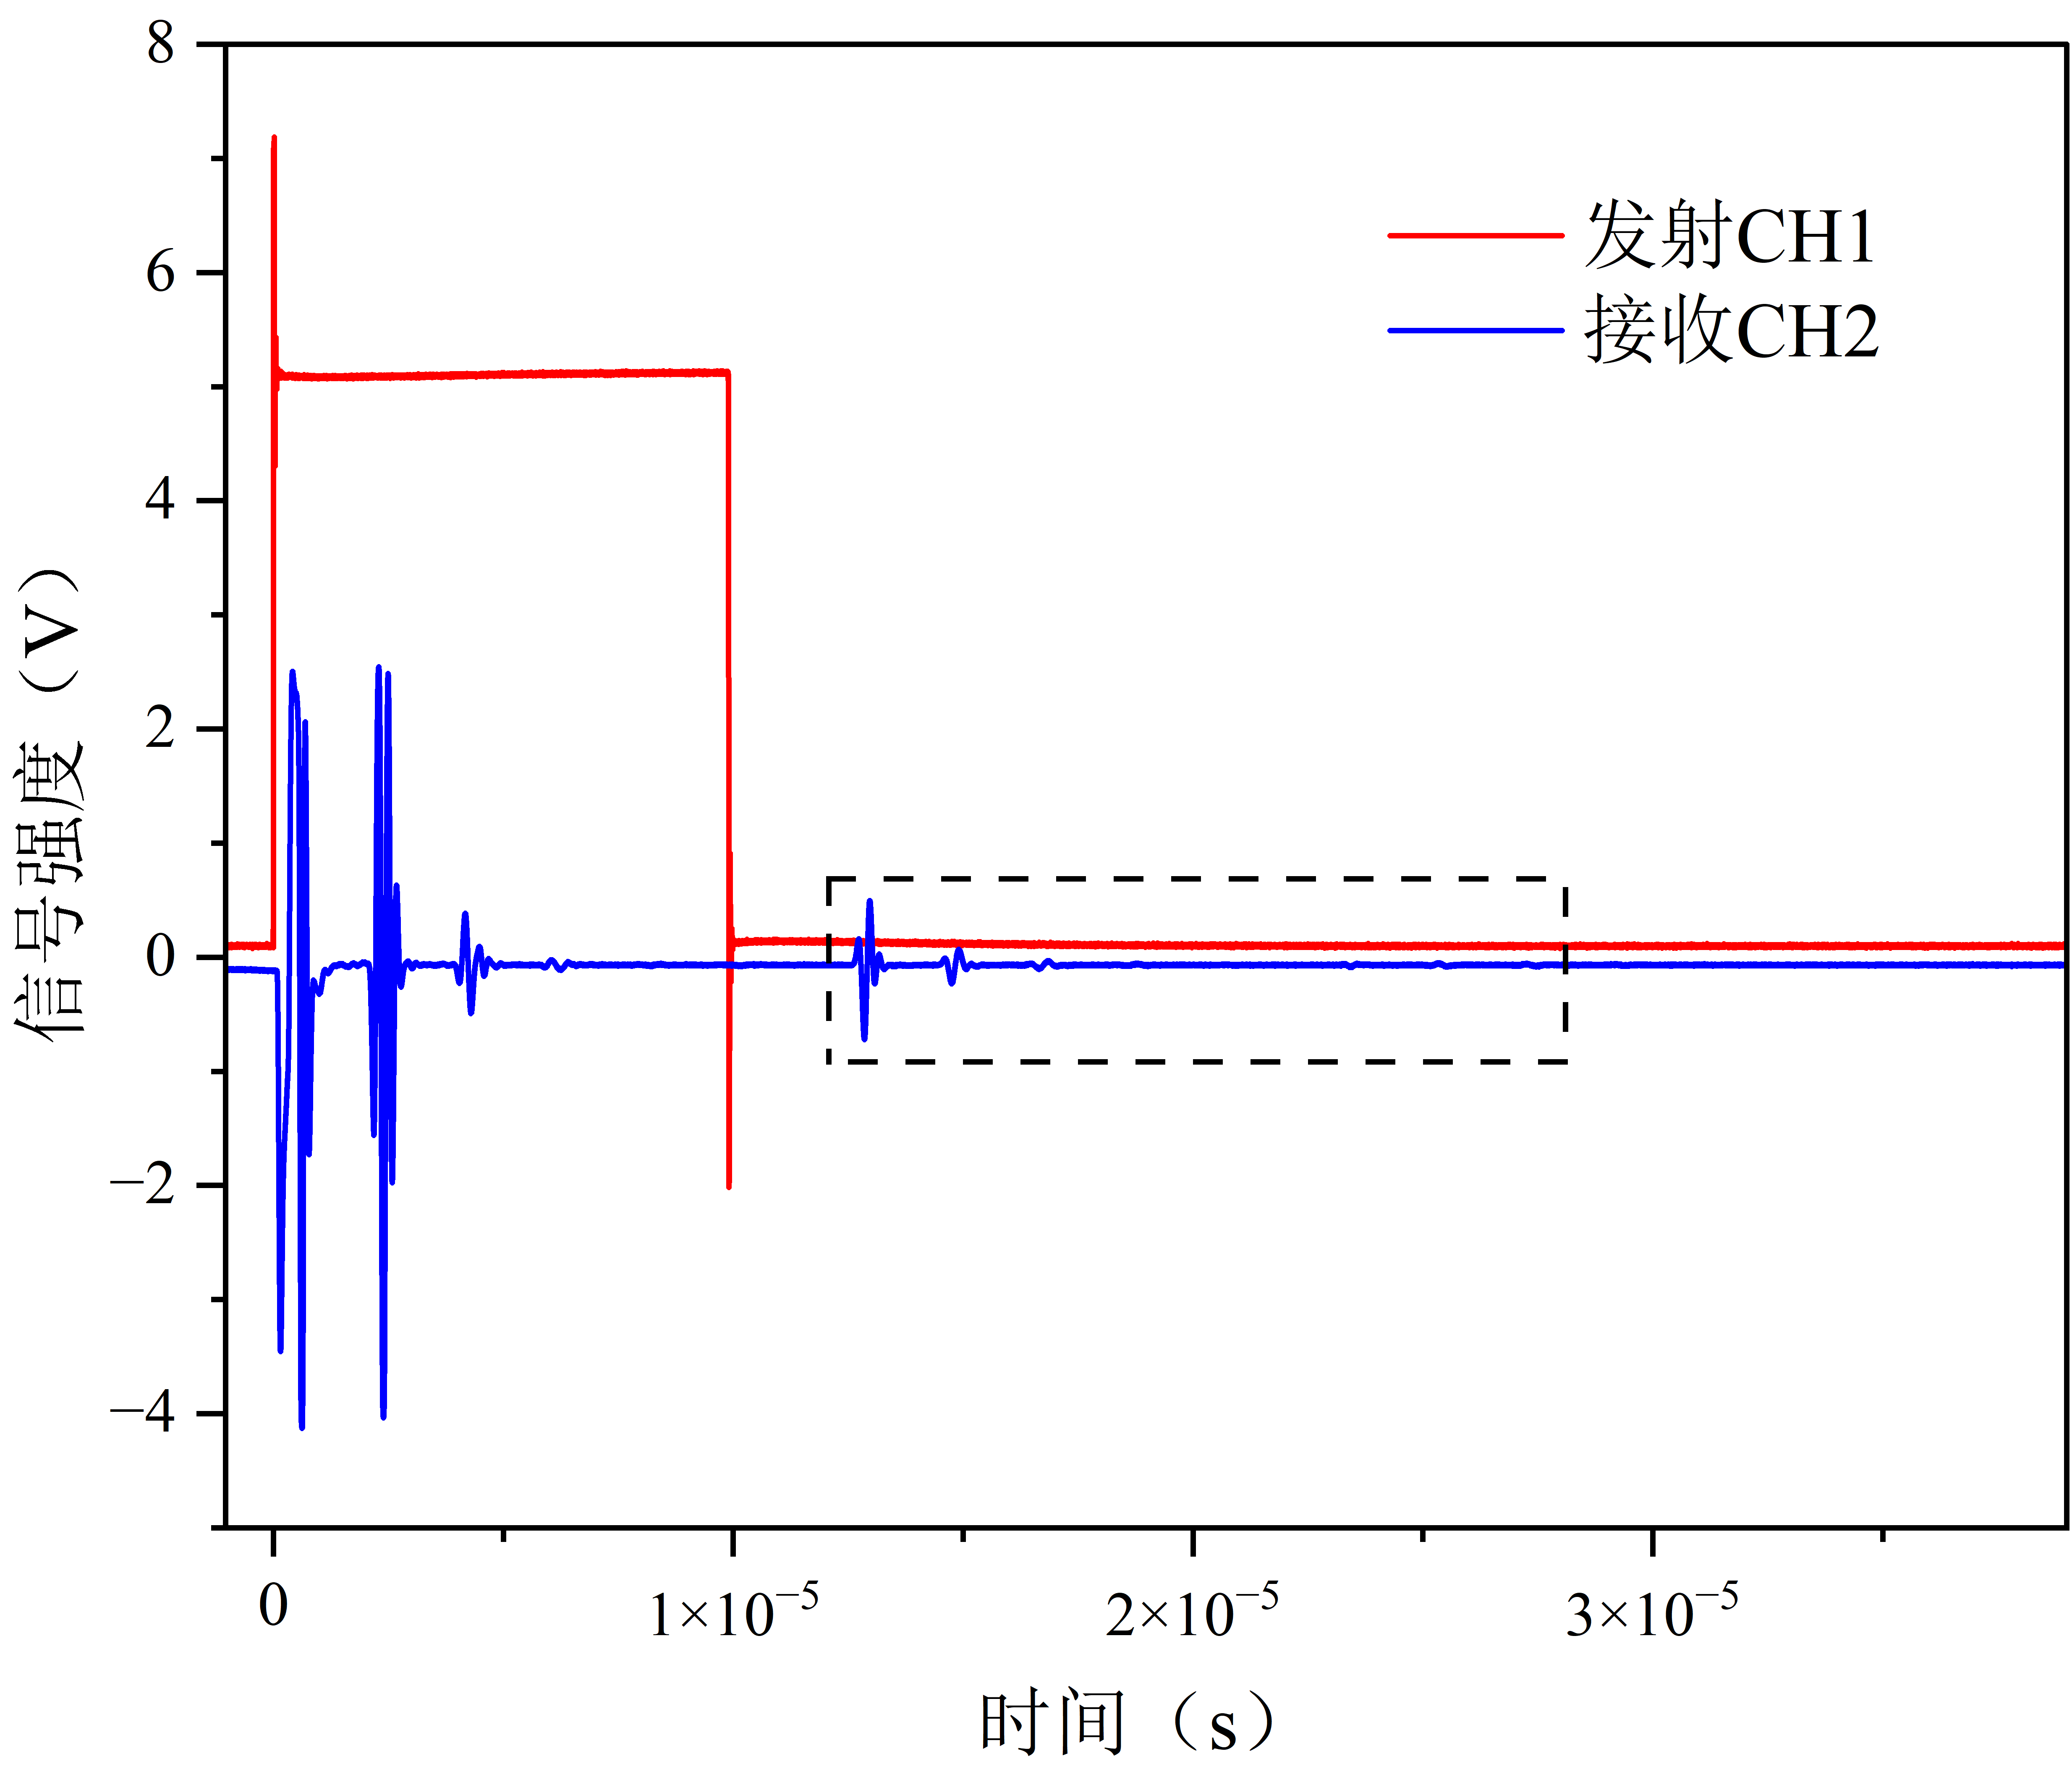
\includegraphics[width=\linewidth]{p10_img01.png}}\hfill
\subcaptionbox{输出信号局部放大图}[0.48\textwidth]{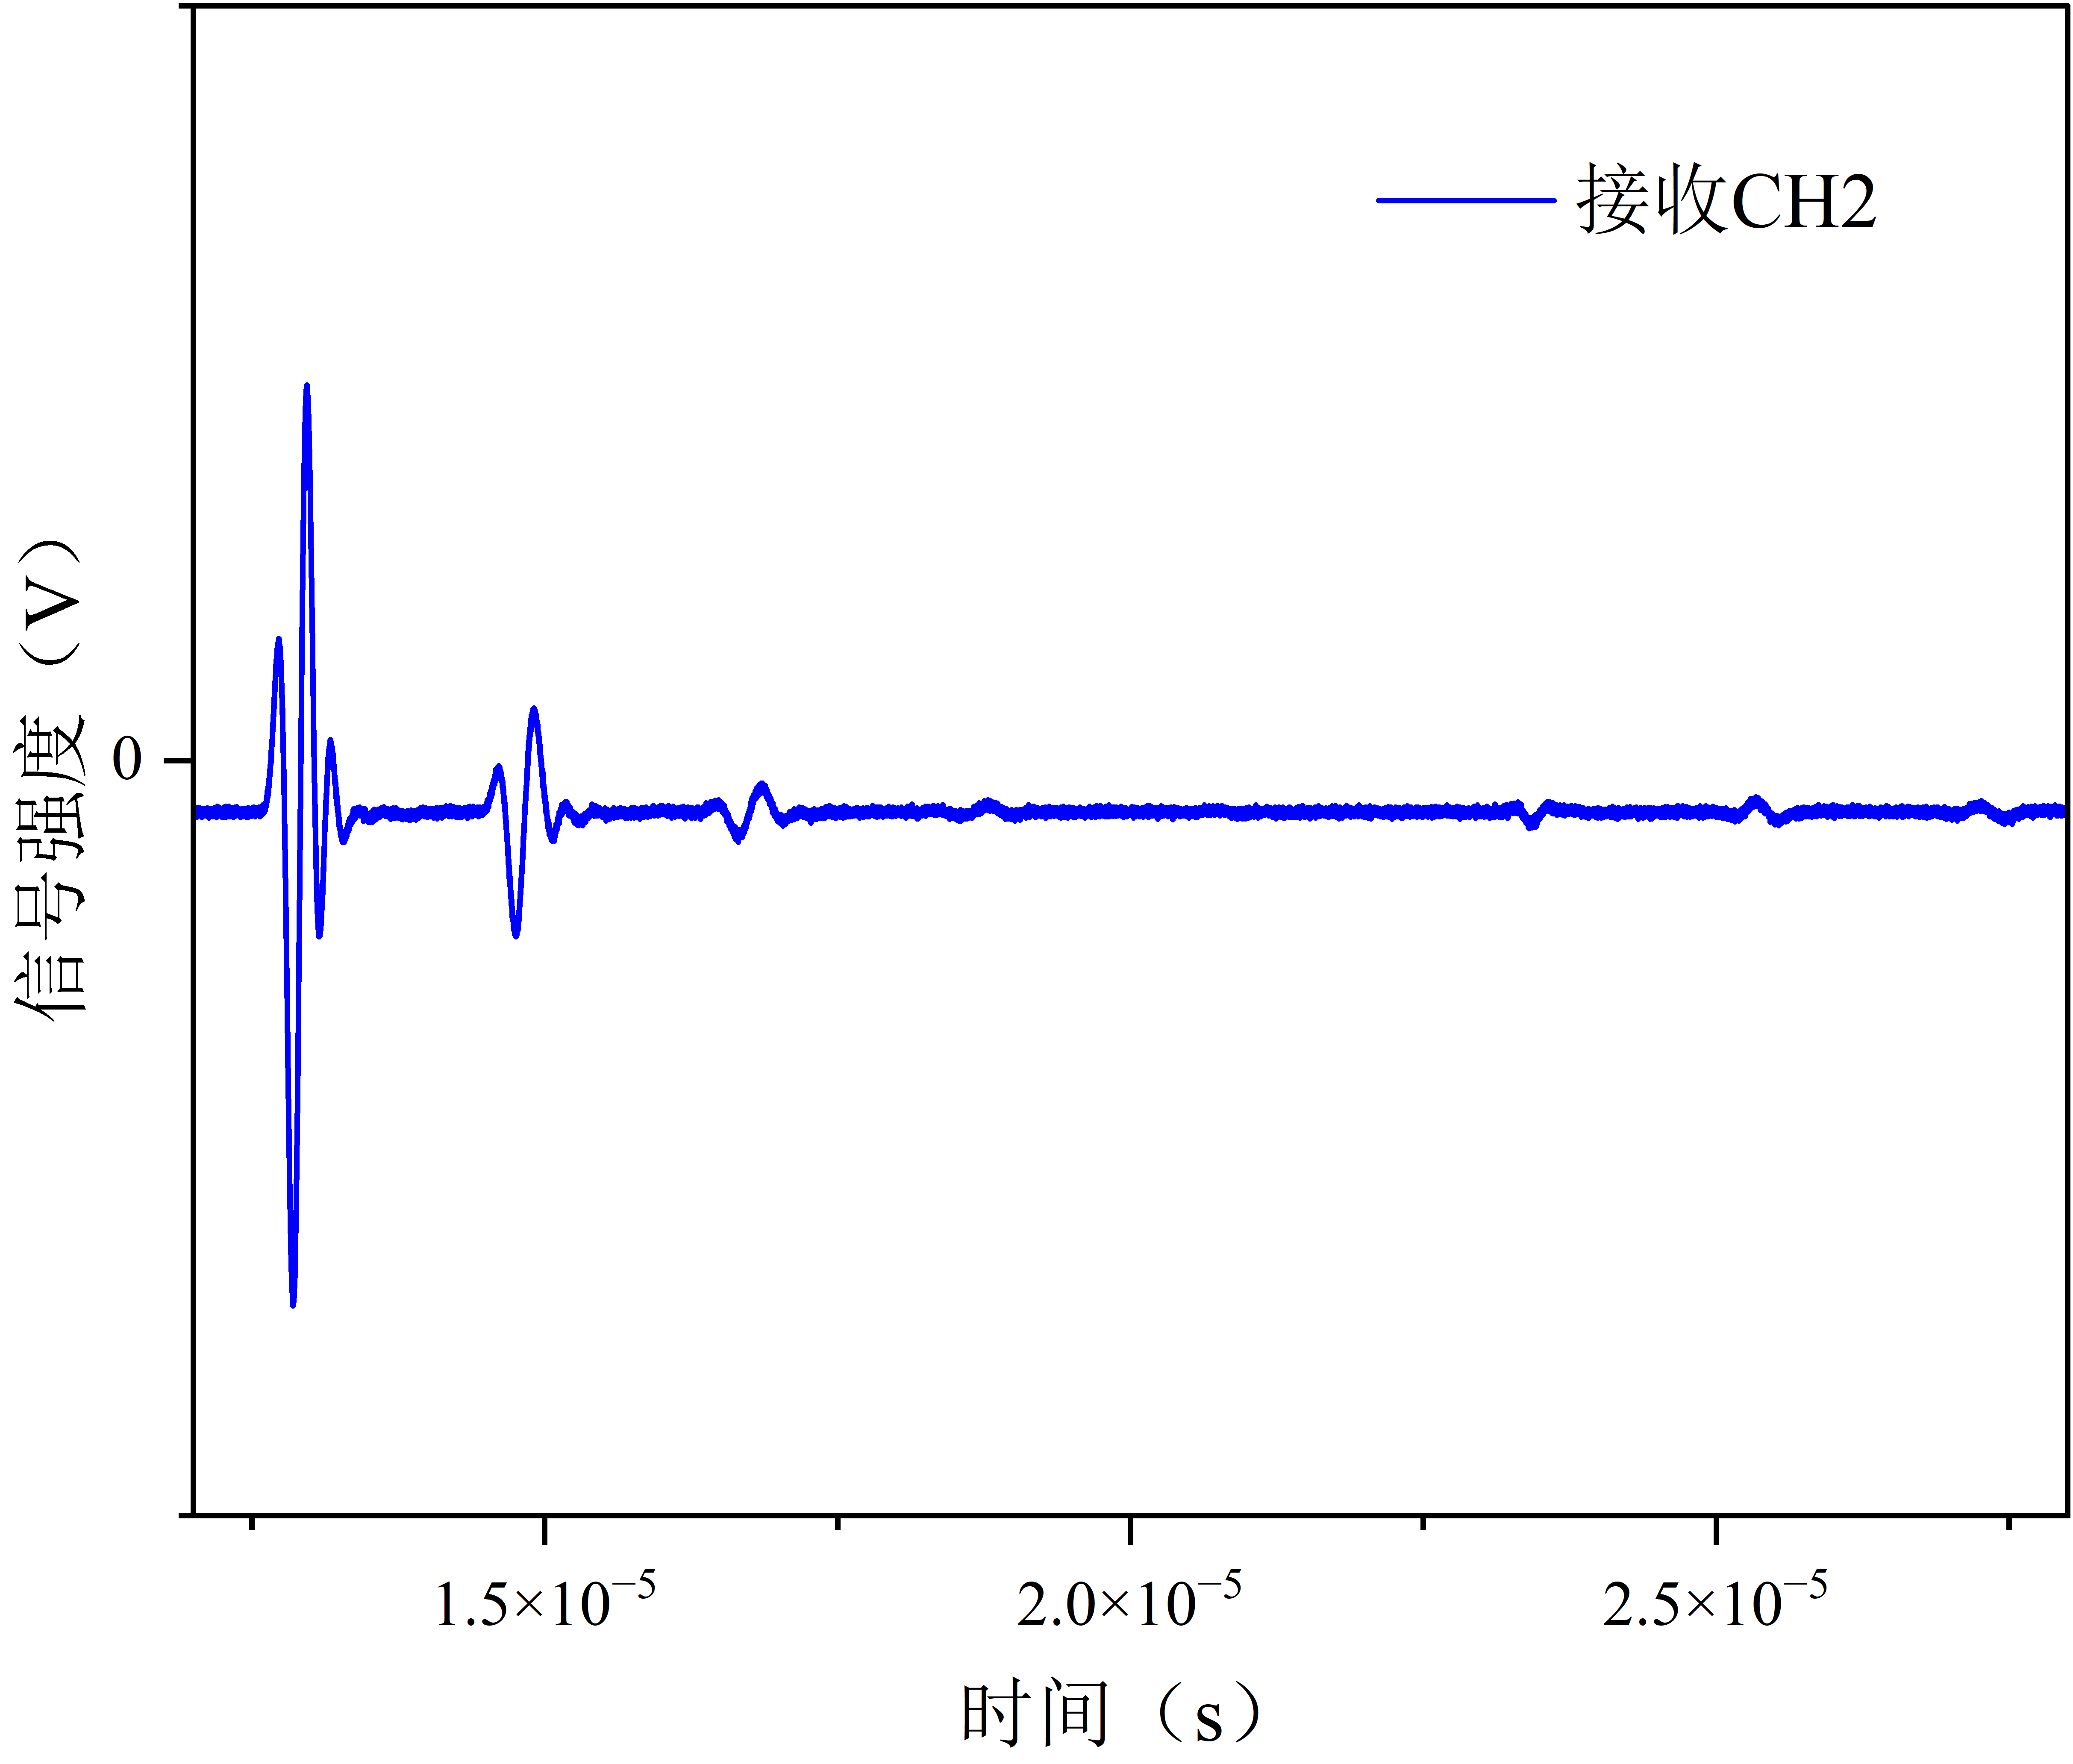
\includegraphics[width=\linewidth]{p10_img02.png}}
\caption{5 MHz 水浸式测量有机玻璃试件纵波波速时信号图}
\label{fig:exp2-og-L}
\end{figure}

\begin{table}[H]
\centering\scriptsize
\caption{5 MHz 水浸式测量三种介质中纵波波峰时间差}
\label{tab:exp2-L-time}
\setlength{\tabcolsep}{3pt}
\begin{tabular}{lccccccc}
\toprule
测量对象 & 测量1 & 测量2 & 测量3 & 均值 & $u_A$ & $u_B$ & $u$\\
\midrule
钢 $\Delta t$（$\mu$s） & \blank[0.8cm] & \blank[0.8cm] & \blank[0.8cm] & \blank[0.8cm] & \blank[0.9cm] & \blank[0.6cm] & \blank[0.9cm]\\
铝 $\Delta t$（$\mu$s） & \blank[0.8cm] & \blank[0.8cm] & \blank[0.8cm] & \blank[0.8cm] & \blank[0.9cm] & \blank[0.6cm] & \blank[0.9cm]\\
有机玻璃 $\Delta t$（$\mu$s） & \blank[0.8cm] & \blank[0.8cm] & \blank[0.8cm] & \blank[0.8cm] & \blank[0.9cm] & \blank[0.6cm] & \blank[0.9cm]\\
\bottomrule
\end{tabular}
\end{table}

由表\ref{tab:exp2-density}和表\ref{tab:exp2-L-time}计算三种介质中的纵波波速：
\begin{subequations}
\begin{align}
  C_{L,st}&=\bar{C}_{L,st}\pm u(C_{L,st})=(\blank[1.4cm]\pm\blank[1.2cm])\ \mathrm{m/s},\\
  C_{L,al}&=\bar{C}_{L,al}\pm u(C_{L,al})=(\blank[1.4cm]\pm\blank[1.2cm])\ \mathrm{m/s},\\
  C_{L,og}&=\bar{C}_{L,og}\pm u(C_{L,og})=(\blank[1.4cm]\pm\blank[1.2cm])\ \mathrm{m/s}.
\end{align}
\end{subequations}
钢、铝和有机玻璃的纵波波速参考值分别为 5900、6300 和 2730 m/s，相对误差为
\begin{subequations}
\begin{align}
  \Delta_{st}&=\frac{|C_{st}-C|}{C}\times100\%=\blank[1.8cm],\\
  \Delta_{al}&=\frac{|C_{al}-C|}{C}\times100\%=\blank[1.8cm],\\
  \Delta_{og}&=\frac{|C_{og}-C|}{C}\times100\%=\blank[1.8cm].
\end{align}
\end{subequations}
结合信号强度、材料非均匀性和波峰读数分析误差。
\answer

\subsection{水浸式测量三种材料的衰减系数}
利用试件上下表面反射波振幅的关系，可以得到纵波在不同介质中的衰减系数。基于图\ref{fig:exp2-steel-L}--图\ref{fig:exp2-og-L}读取不同时间下的波峰数值。将所得波峰幅值数据代入公式\eqref{eq:exp2-attenuation}，结合表\ref{tab:exp2-density}中的数据，结果填入表\ref{tab:exp2-attenuation}。

\begin{table}[H]
\centering\small
\caption{5 MHz 水浸式测量三种介质中纵波波峰及衰减系数}
\label{tab:exp2-attenuation}
\begin{tabular}{lcccc}
\toprule
测量对象 & $P_m$（V） & $P_n$（V） & $\bar{\alpha}$（dB/cm） & $u(\alpha)$（dB/cm）\\
\midrule
钢 & \blank[1.3cm]\ ($m=$\blank[0.4cm]) & \blank[1.3cm]\ ($n=$\blank[0.4cm]) & \blank[1.3cm] & \blank[1.3cm]\\
铝 & \blank[1.3cm]\ ($m=$\blank[0.4cm]) & \blank[1.3cm]\ ($n=$\blank[0.4cm]) & \blank[1.3cm] & \blank[1.3cm]\\
有机玻璃 & \blank[1.3cm]\ ($m=$\blank[0.4cm]) & \blank[1.3cm]\ ($n=$\blank[0.4cm]) & \blank[1.3cm] & \blank[1.3cm]\\
\bottomrule
\end{tabular}
\end{table}

纵波在钢、铝、有机玻璃中的平均衰减系数分别为
\begin{subequations}
\begin{align}
  \alpha_{L,st}&=\bar{\alpha}_{L,st}\pm u(\alpha_{L,st})=(\blank[1.3cm]\pm\blank[1.2cm])\ \mathrm{dB/cm},\\
  \alpha_{L,al}&=\bar{\alpha}_{L,al}\pm u(\alpha_{L,al})=(\blank[1.3cm]\pm\blank[1.2cm])\ \mathrm{dB/cm},\\
  \alpha_{L,og}&=\bar{\alpha}_{L,og}\pm u(\alpha_{L,og})=(\blank[1.3cm]\pm\blank[1.2cm])\ \mathrm{dB/cm}.
\end{align}
\end{subequations}
比较三种材料的衰减程度，并分析信号强度对波峰读取和计算结果的影响。
\answer

\subsection{接触式测量三种材料的横波波速}
使用频率为 5 MHz 的横波超声探头进行接触式测量。记录本组增益设置：\blank[2cm]。波形数据及用于计算波速的数据区域如图\ref{fig:exp2-steel-S}--图\ref{fig:exp2-og-S}所示，波峰时间差填入表\ref{tab:exp2-S-time}。

\begin{figure}[H]
\centering
\subcaptionbox{输入输出信号全局图}[0.48\textwidth]{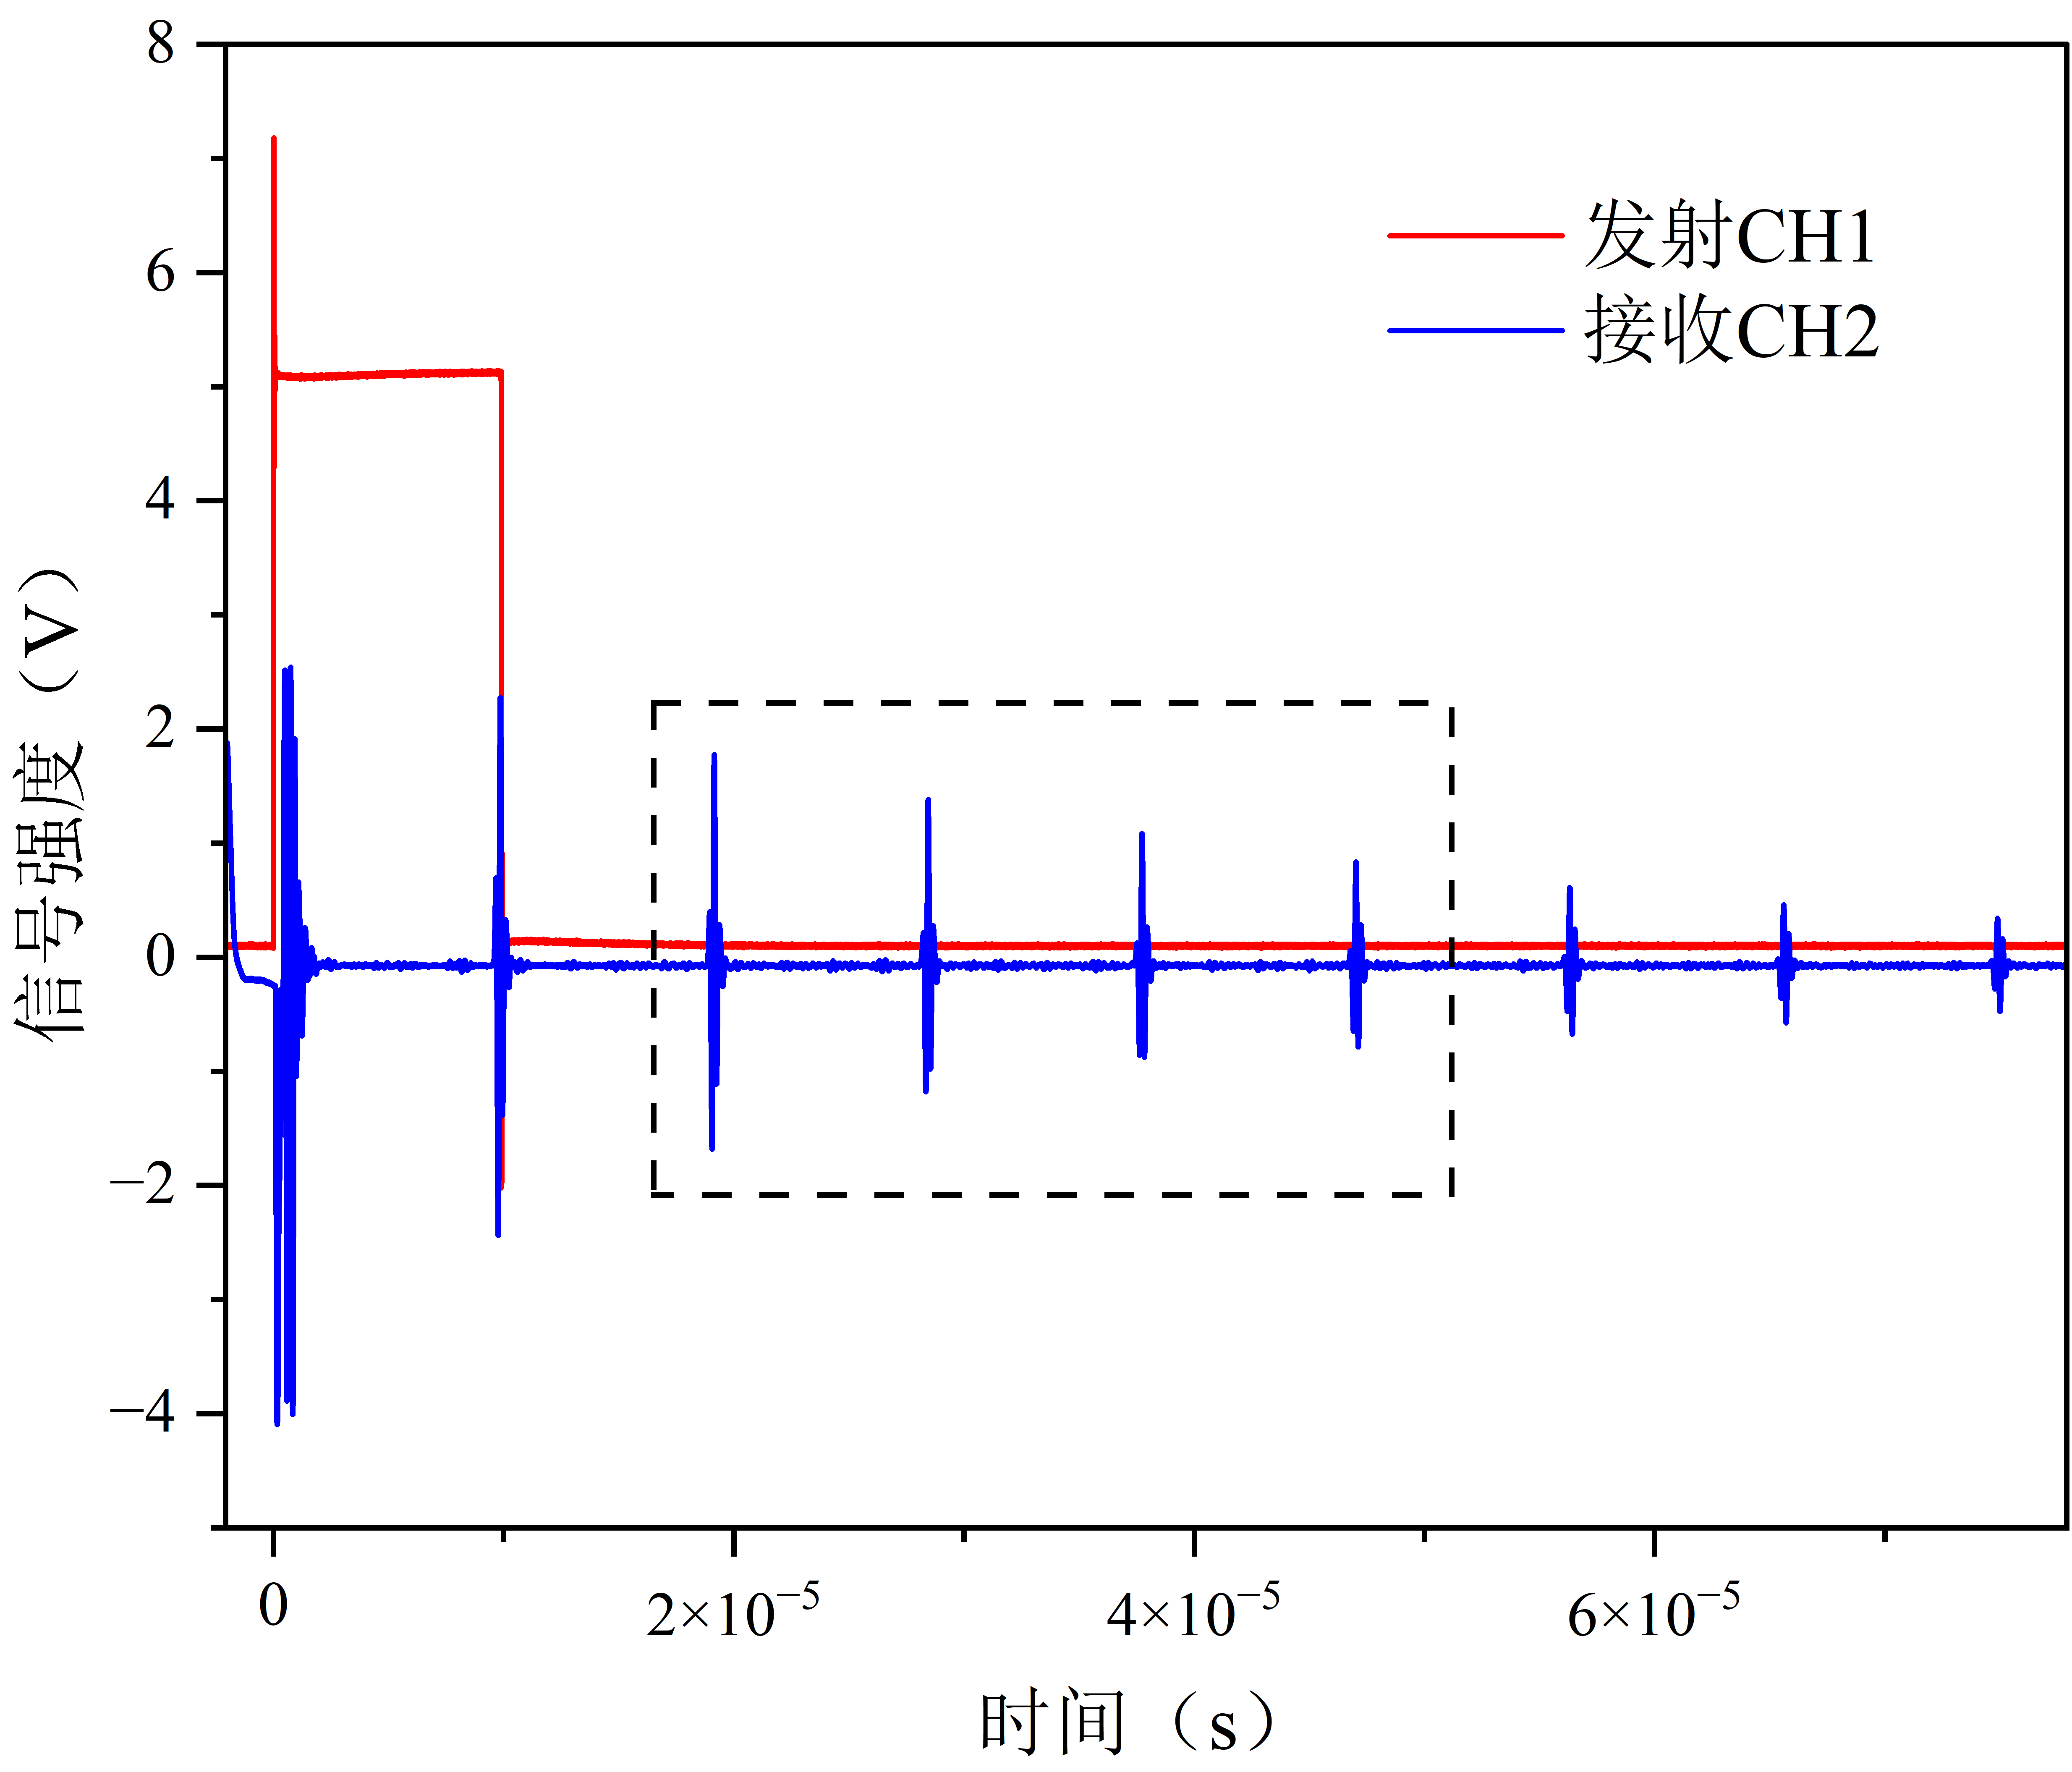
\includegraphics[width=\linewidth]{p11_img01.png}}\hfill
\subcaptionbox{输出信号局部放大图}[0.48\textwidth]{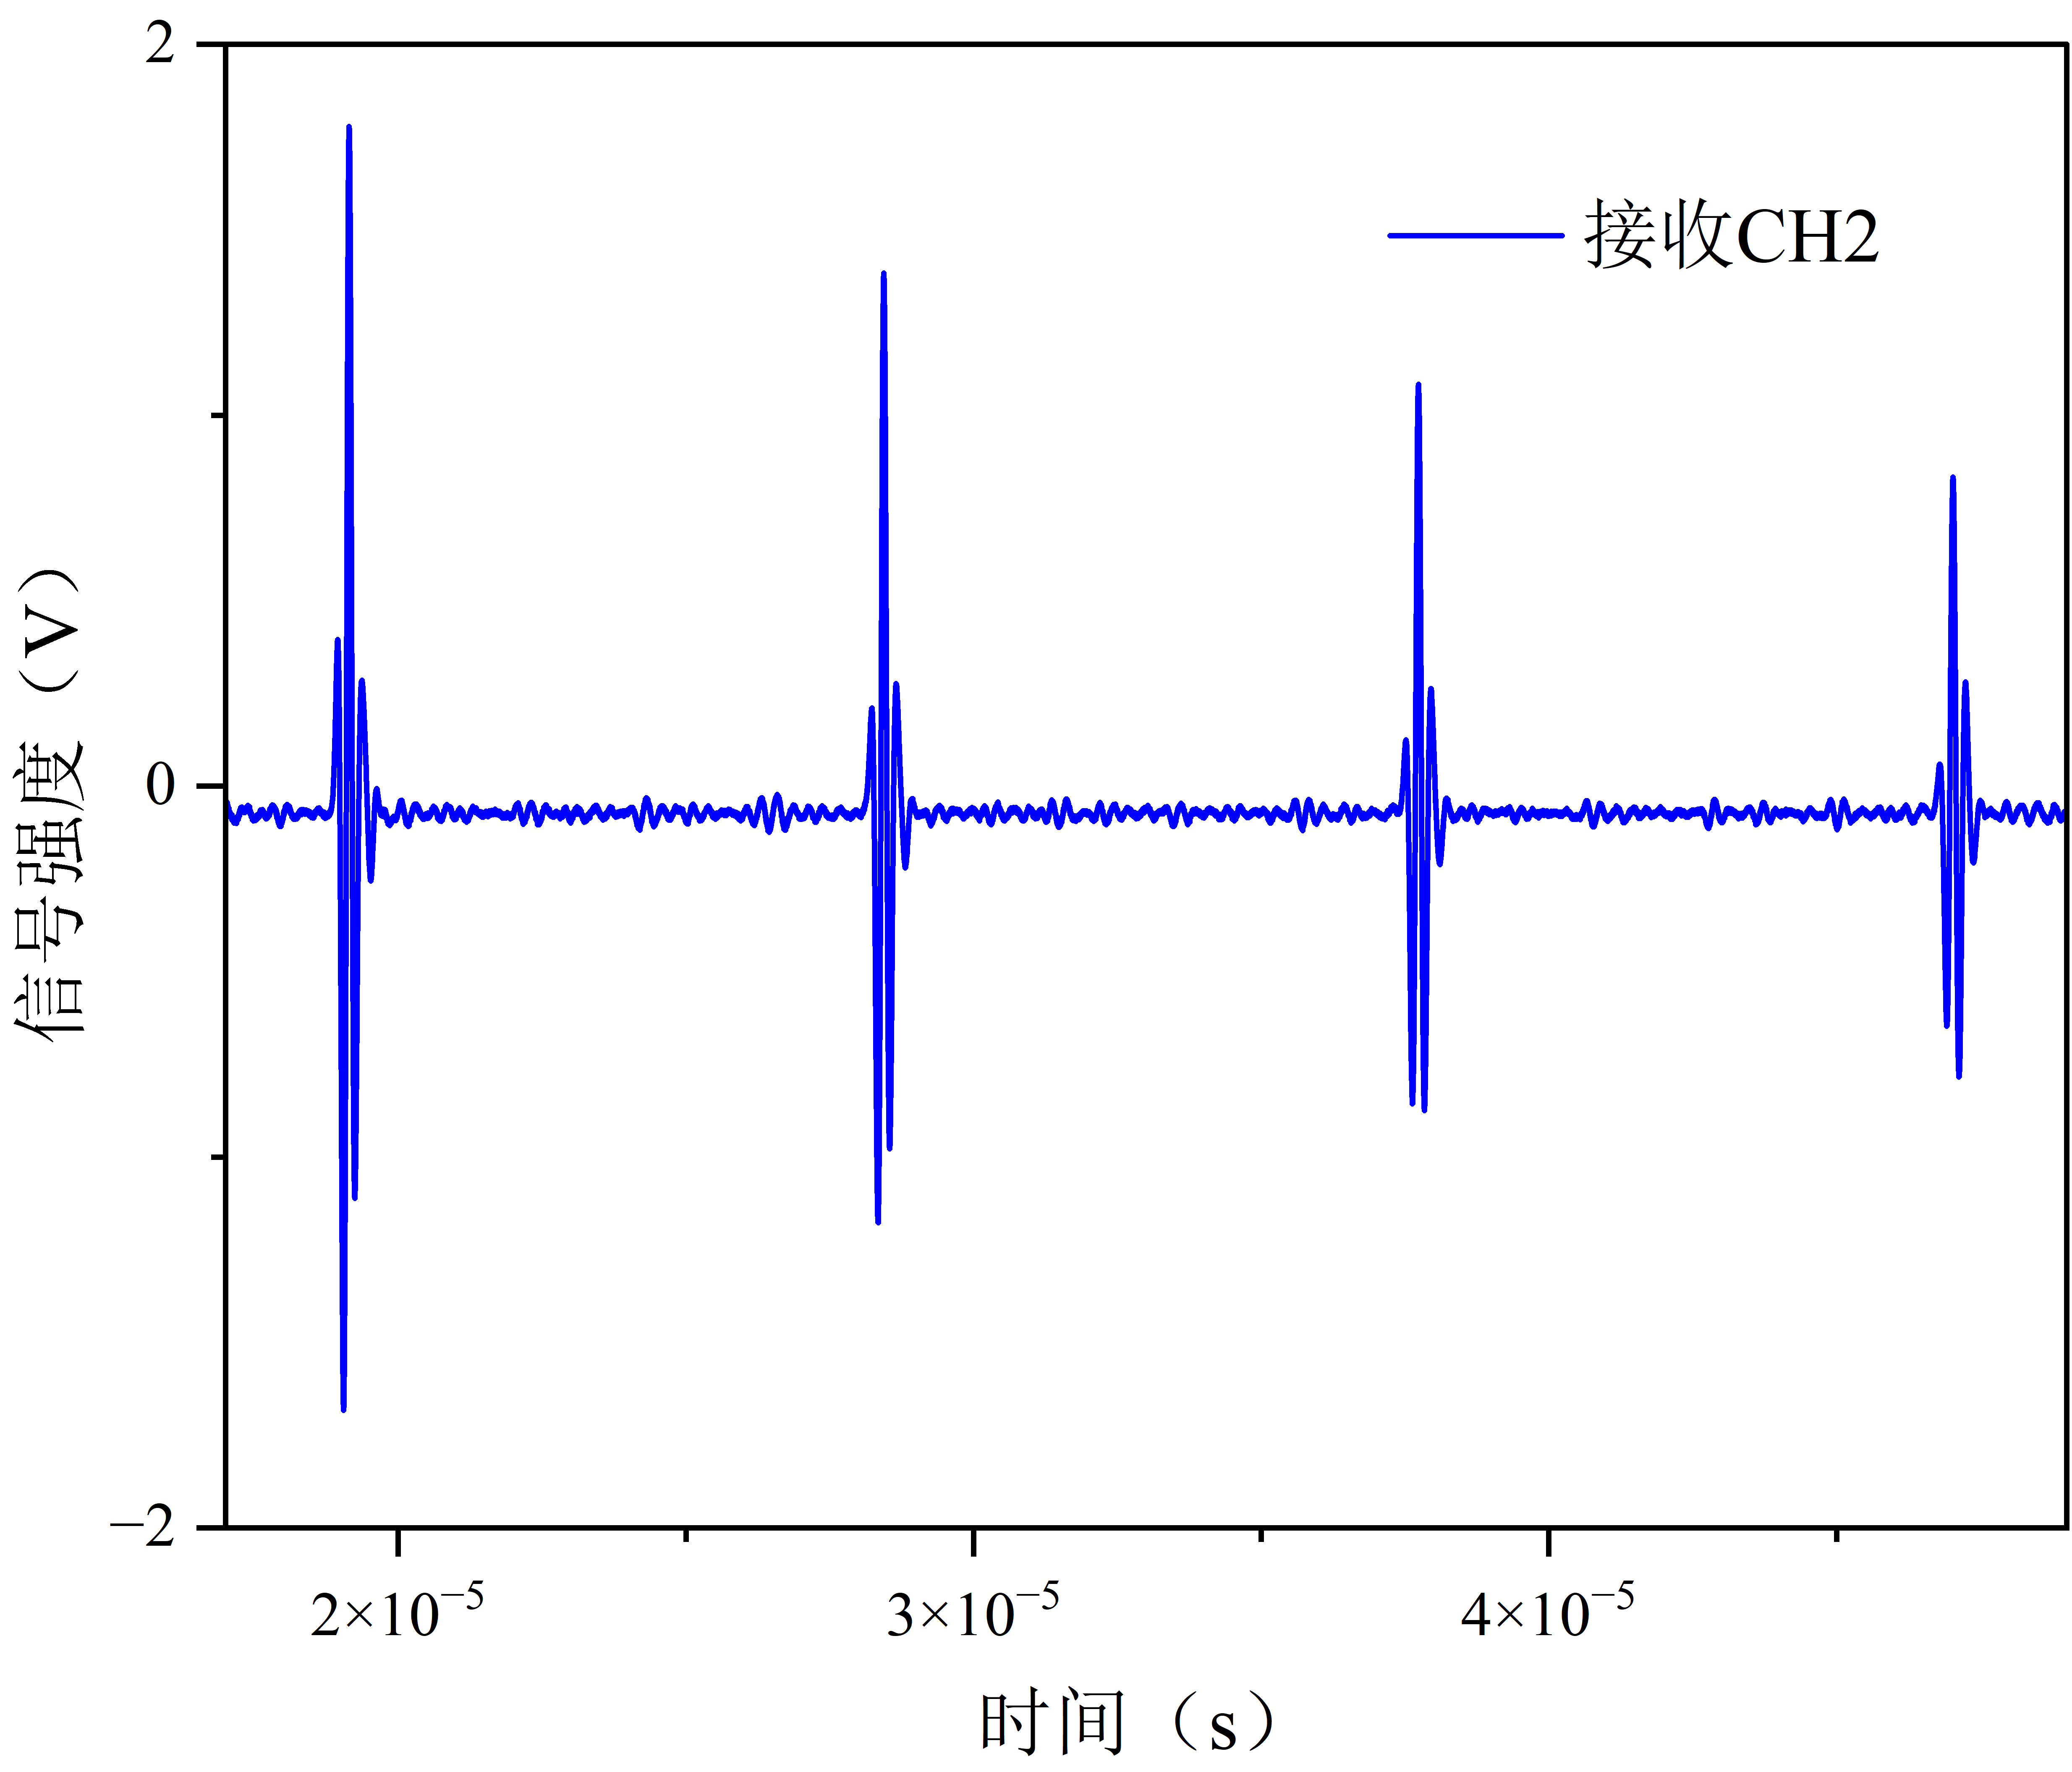
\includegraphics[width=\linewidth]{p11_img02.png}}
\caption{5 MHz 接触式测量钢试件横波波速时信号图}
\label{fig:exp2-steel-S}
\end{figure}

\begin{figure}[H]
\centering
\subcaptionbox{输入输出信号全局图}[0.48\textwidth]{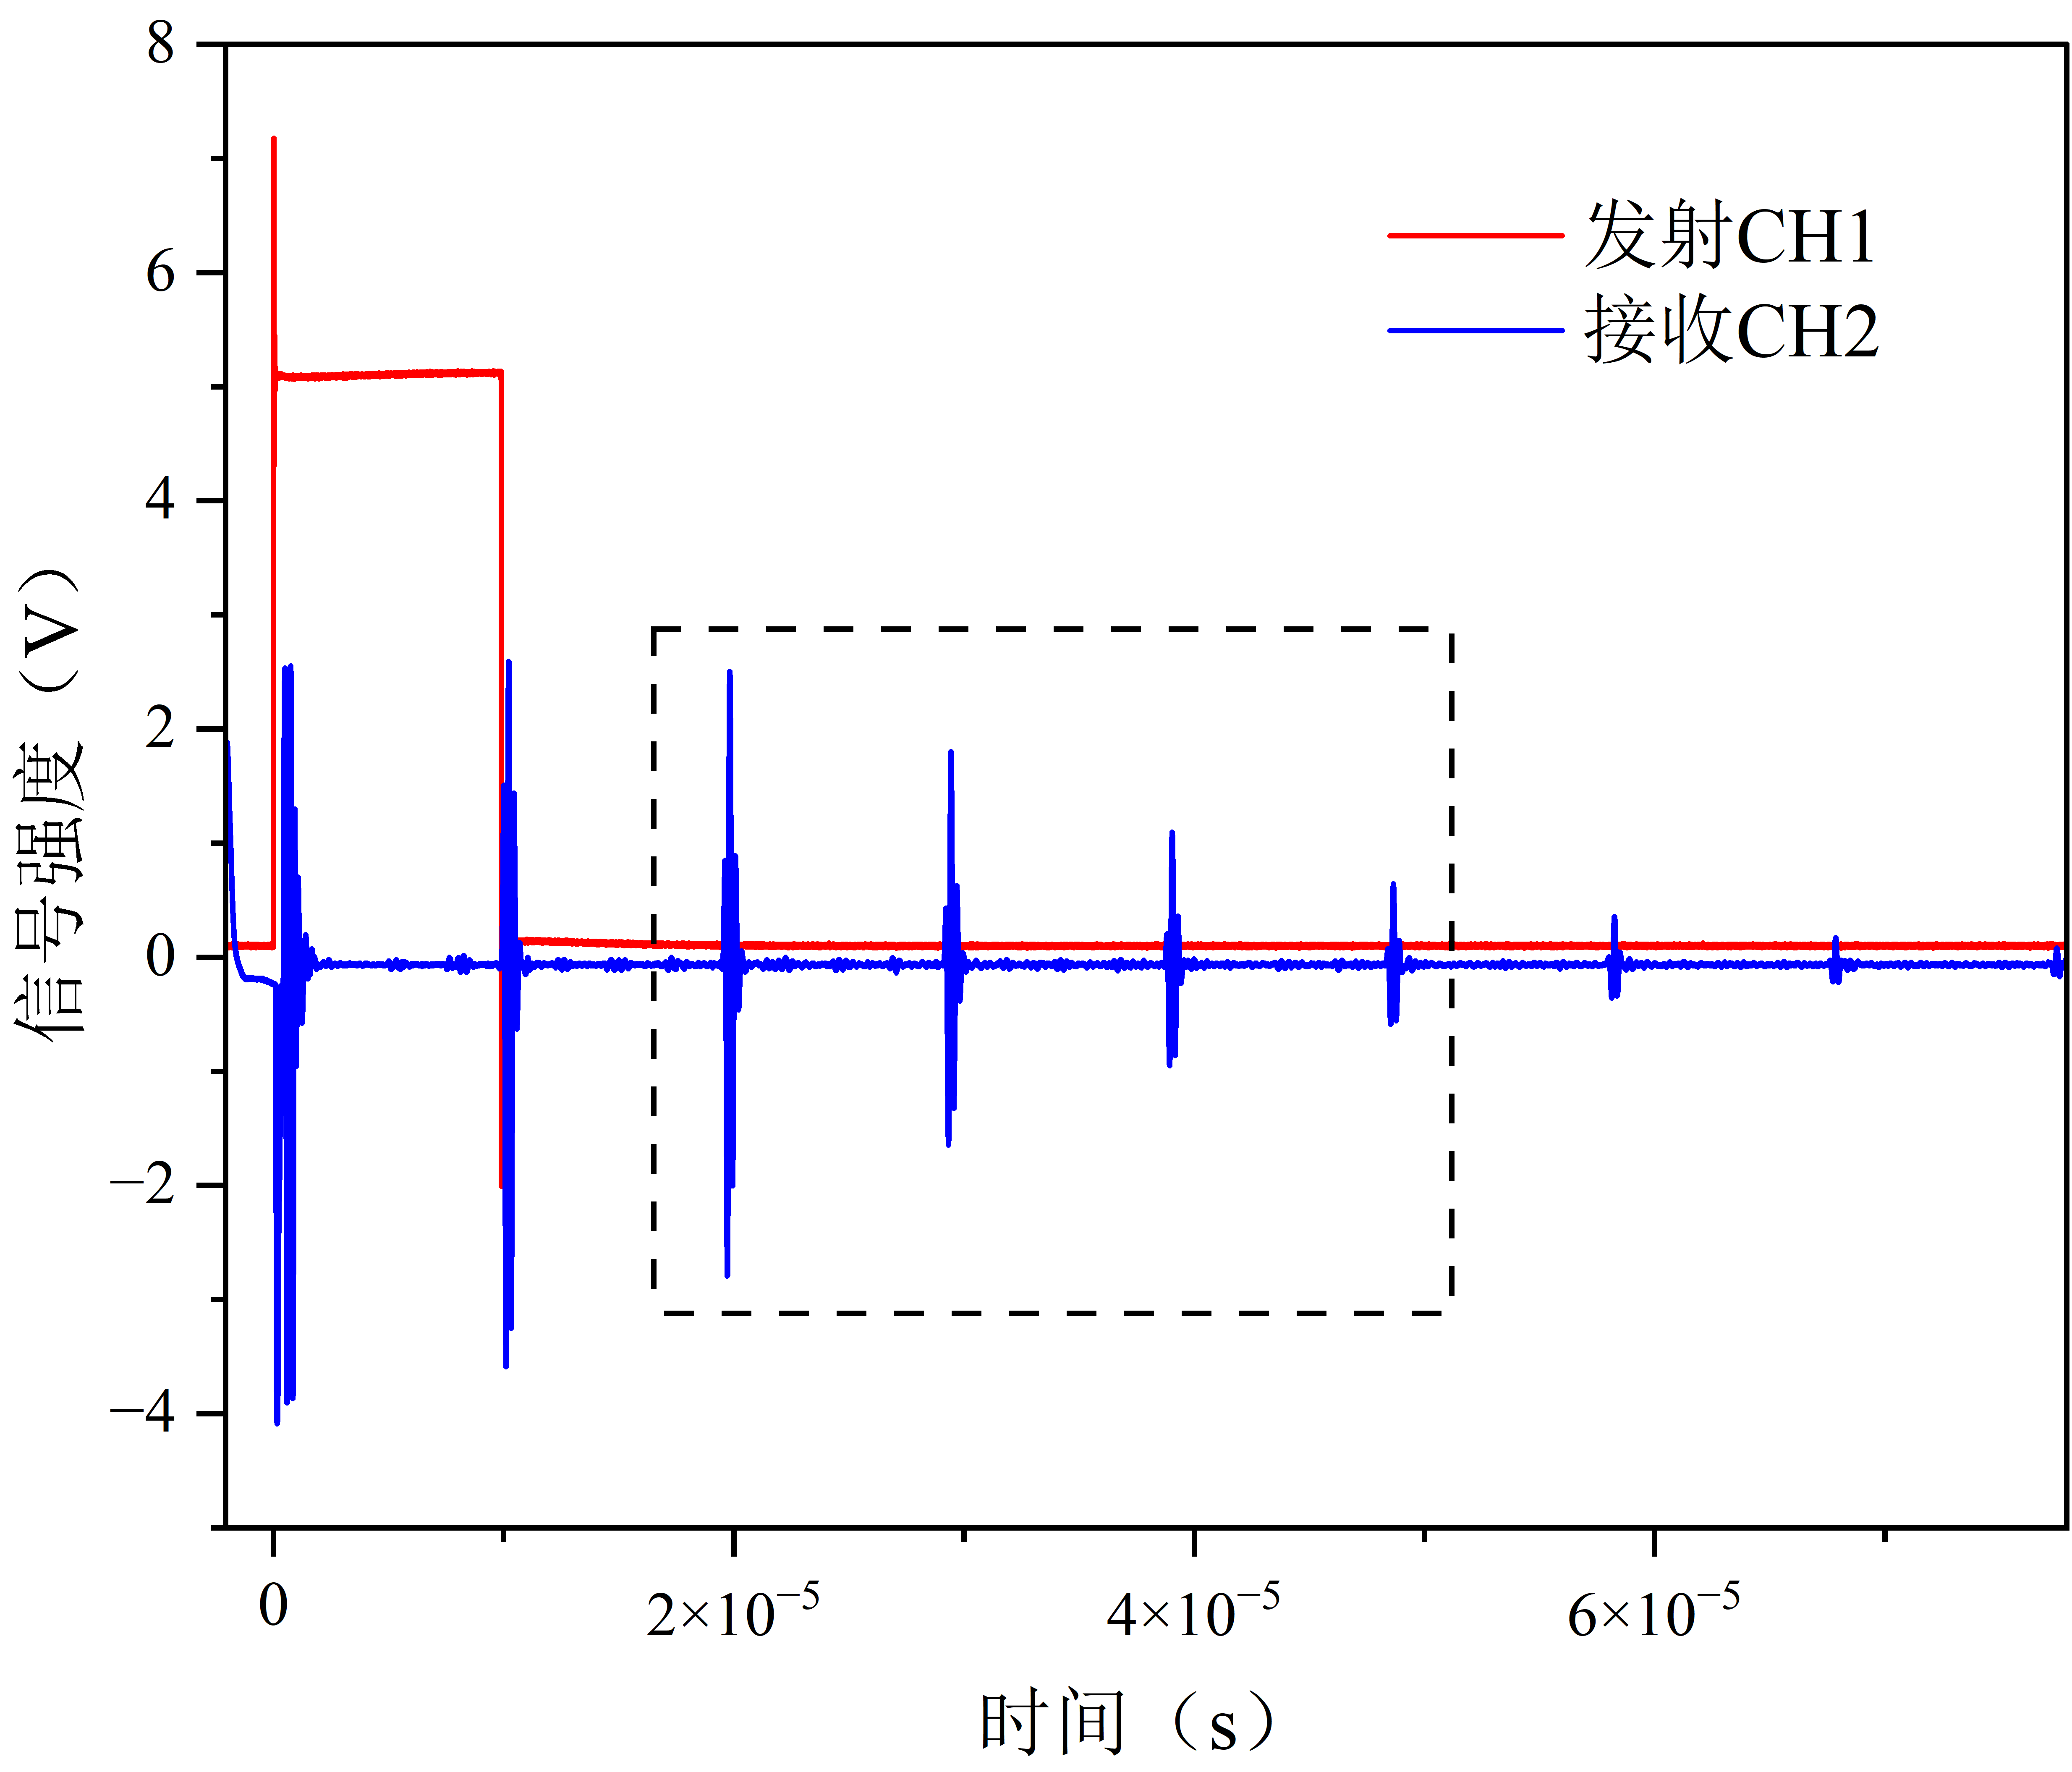
\includegraphics[width=\linewidth]{p12_img01.png}}\hfill
\subcaptionbox{输出信号局部放大图}[0.48\textwidth]{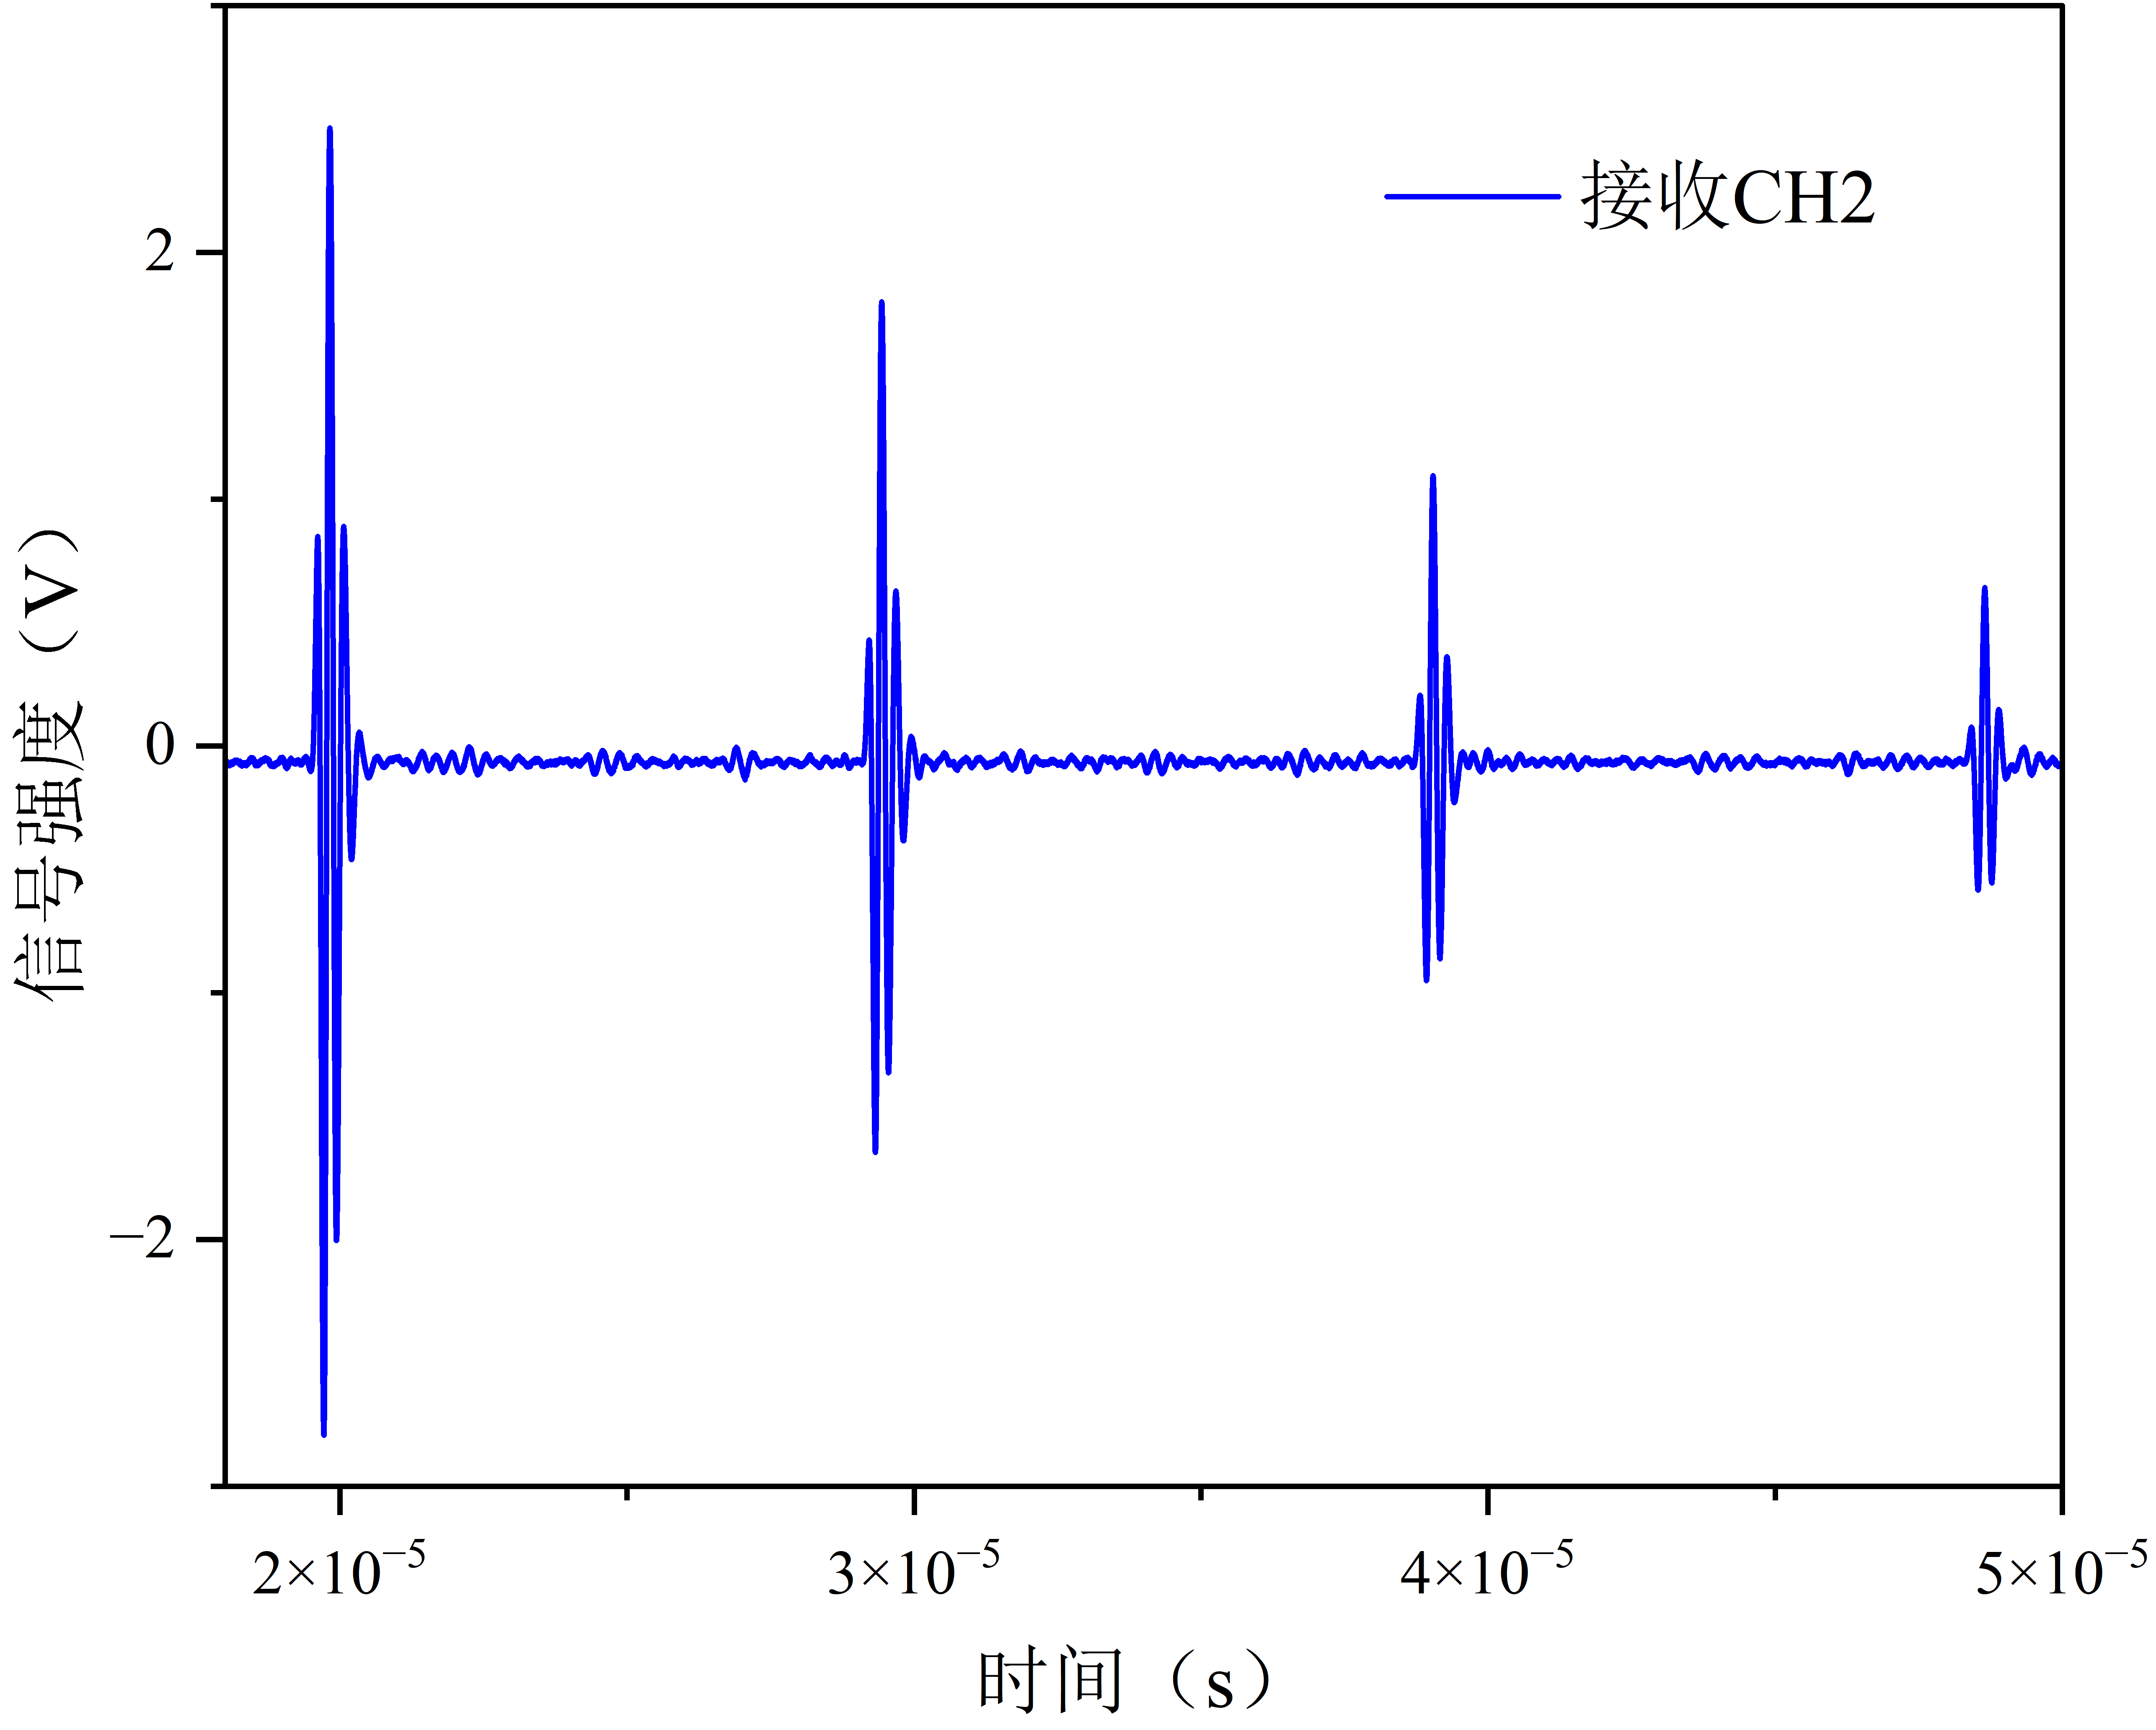
\includegraphics[width=\linewidth]{p12_img02.png}}
\caption{5 MHz 接触式测量铝试件横波波速时信号图}
\end{figure}

\begin{figure}[H]
\centering
\subcaptionbox{输入输出信号全局图}[0.48\textwidth]{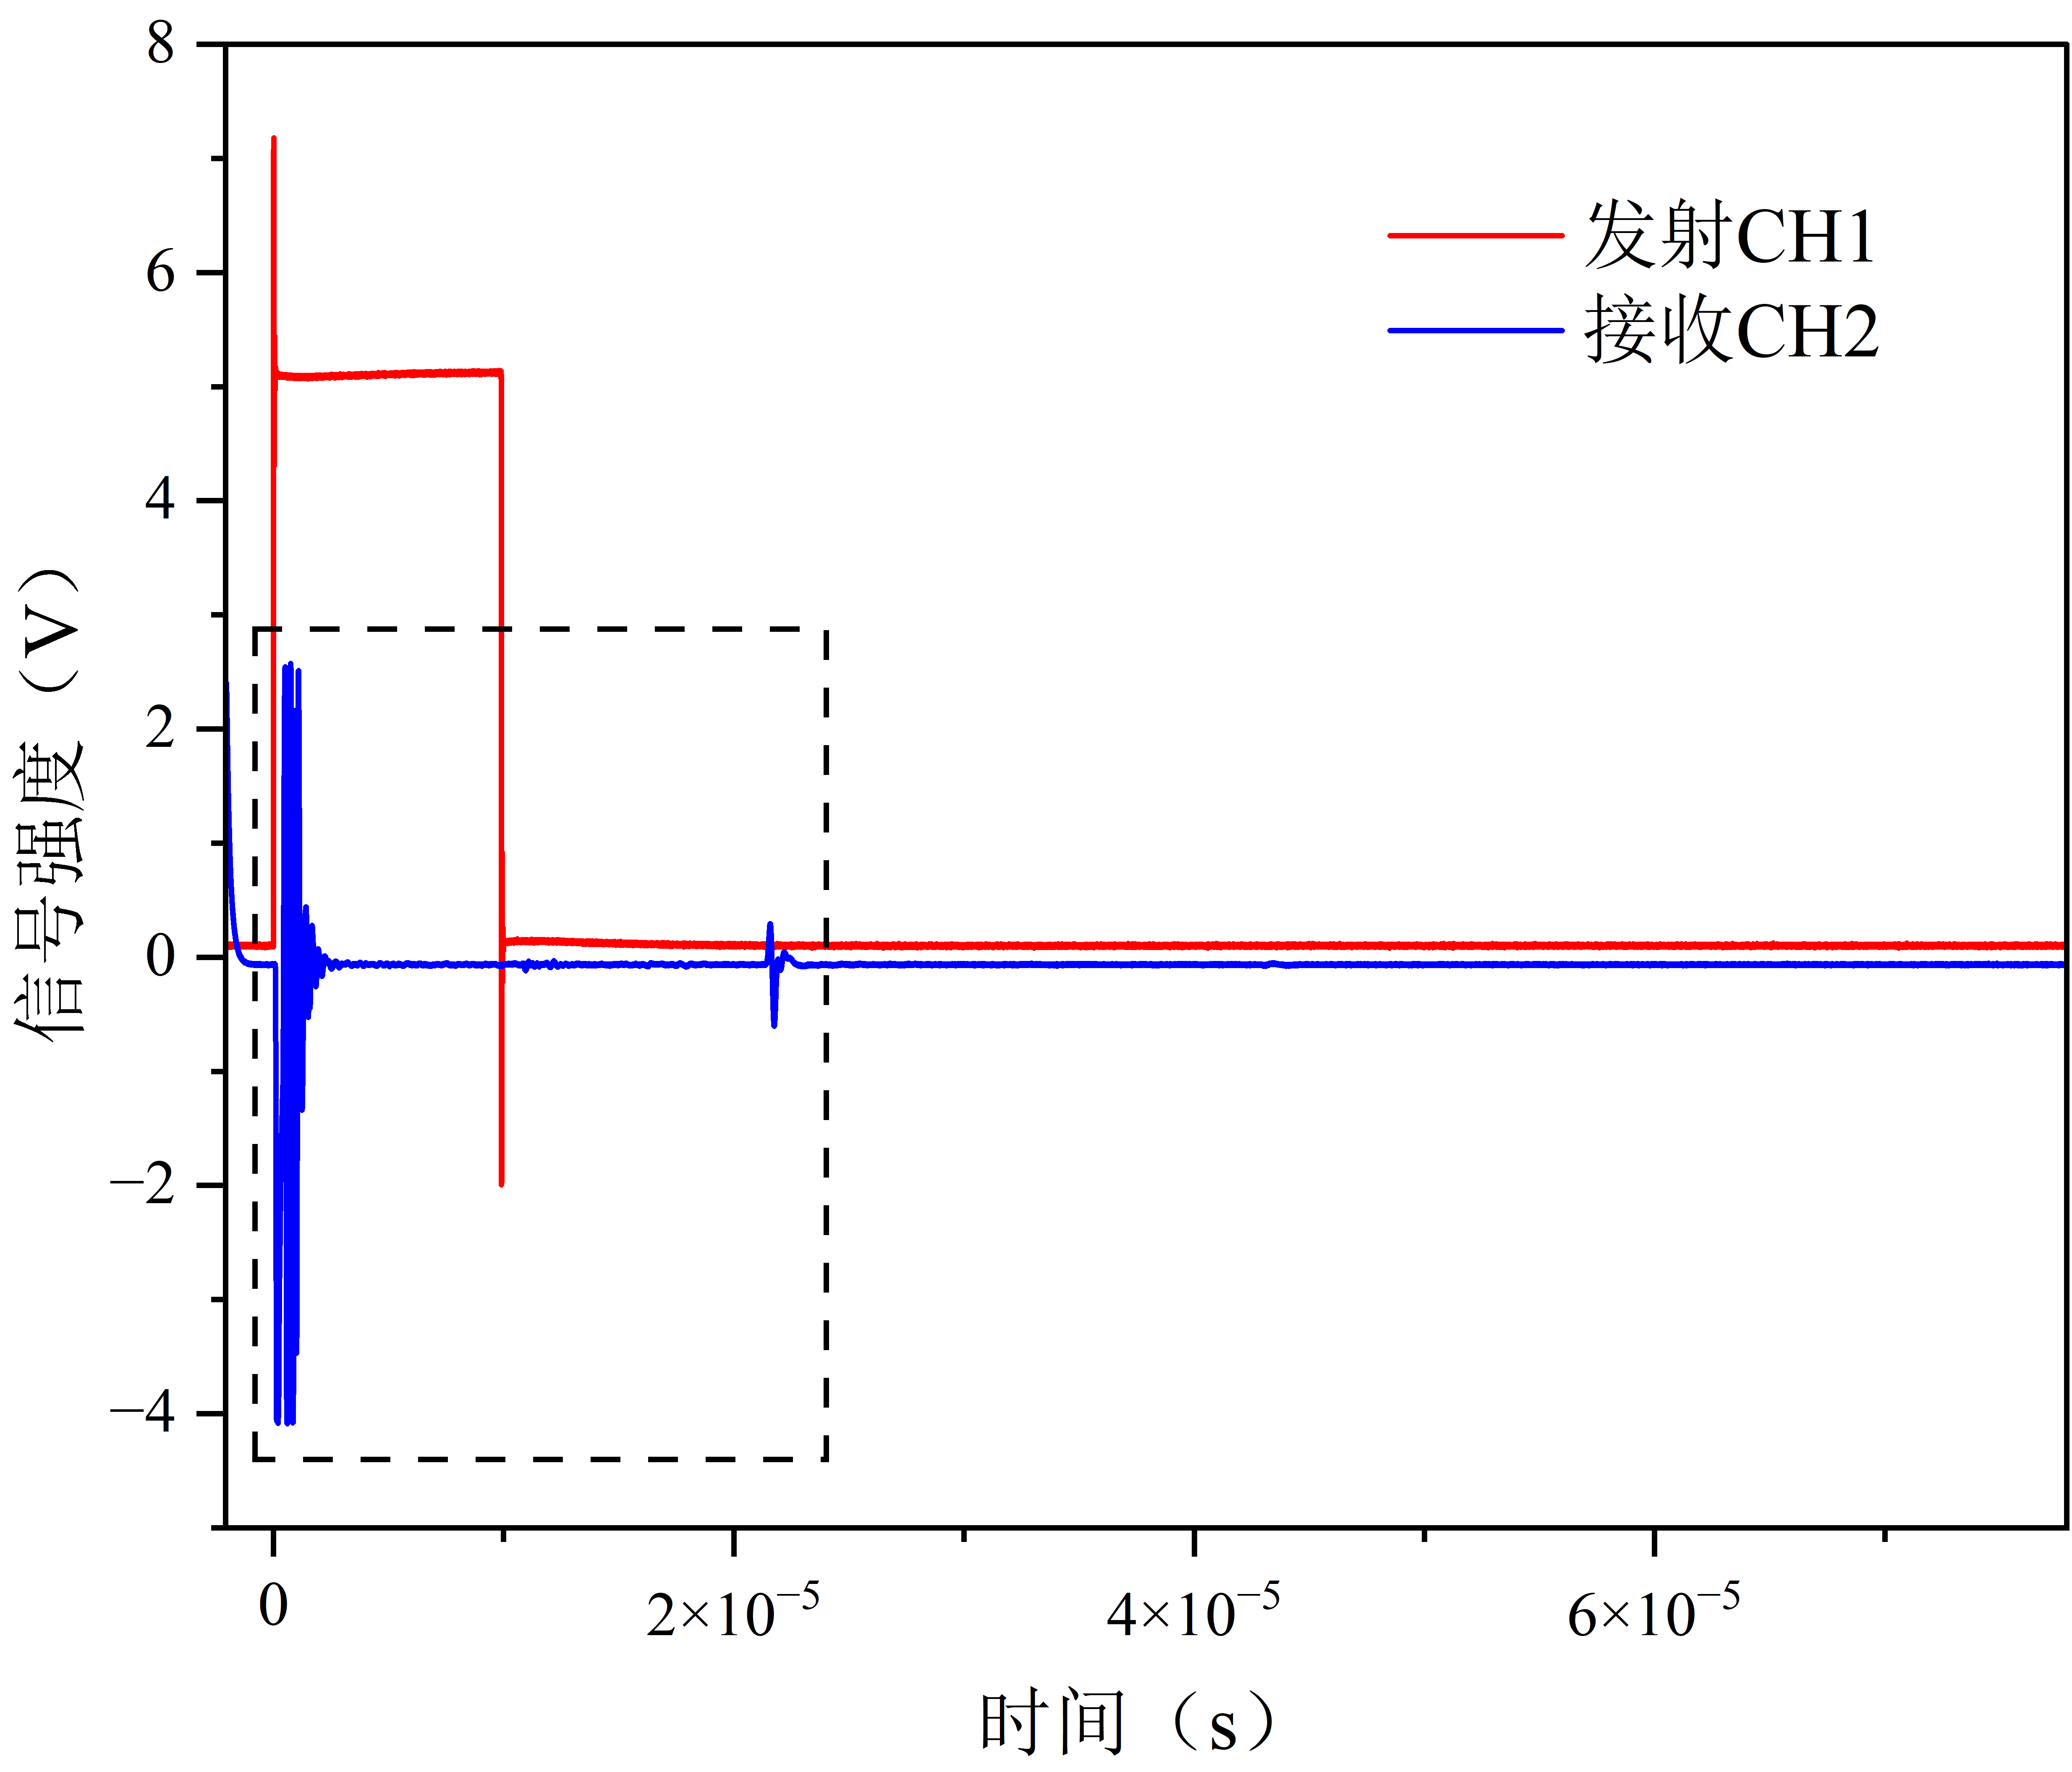
\includegraphics[width=\linewidth]{p13_img01.png}}\hfill
\subcaptionbox{输出信号局部放大图}[0.48\textwidth]{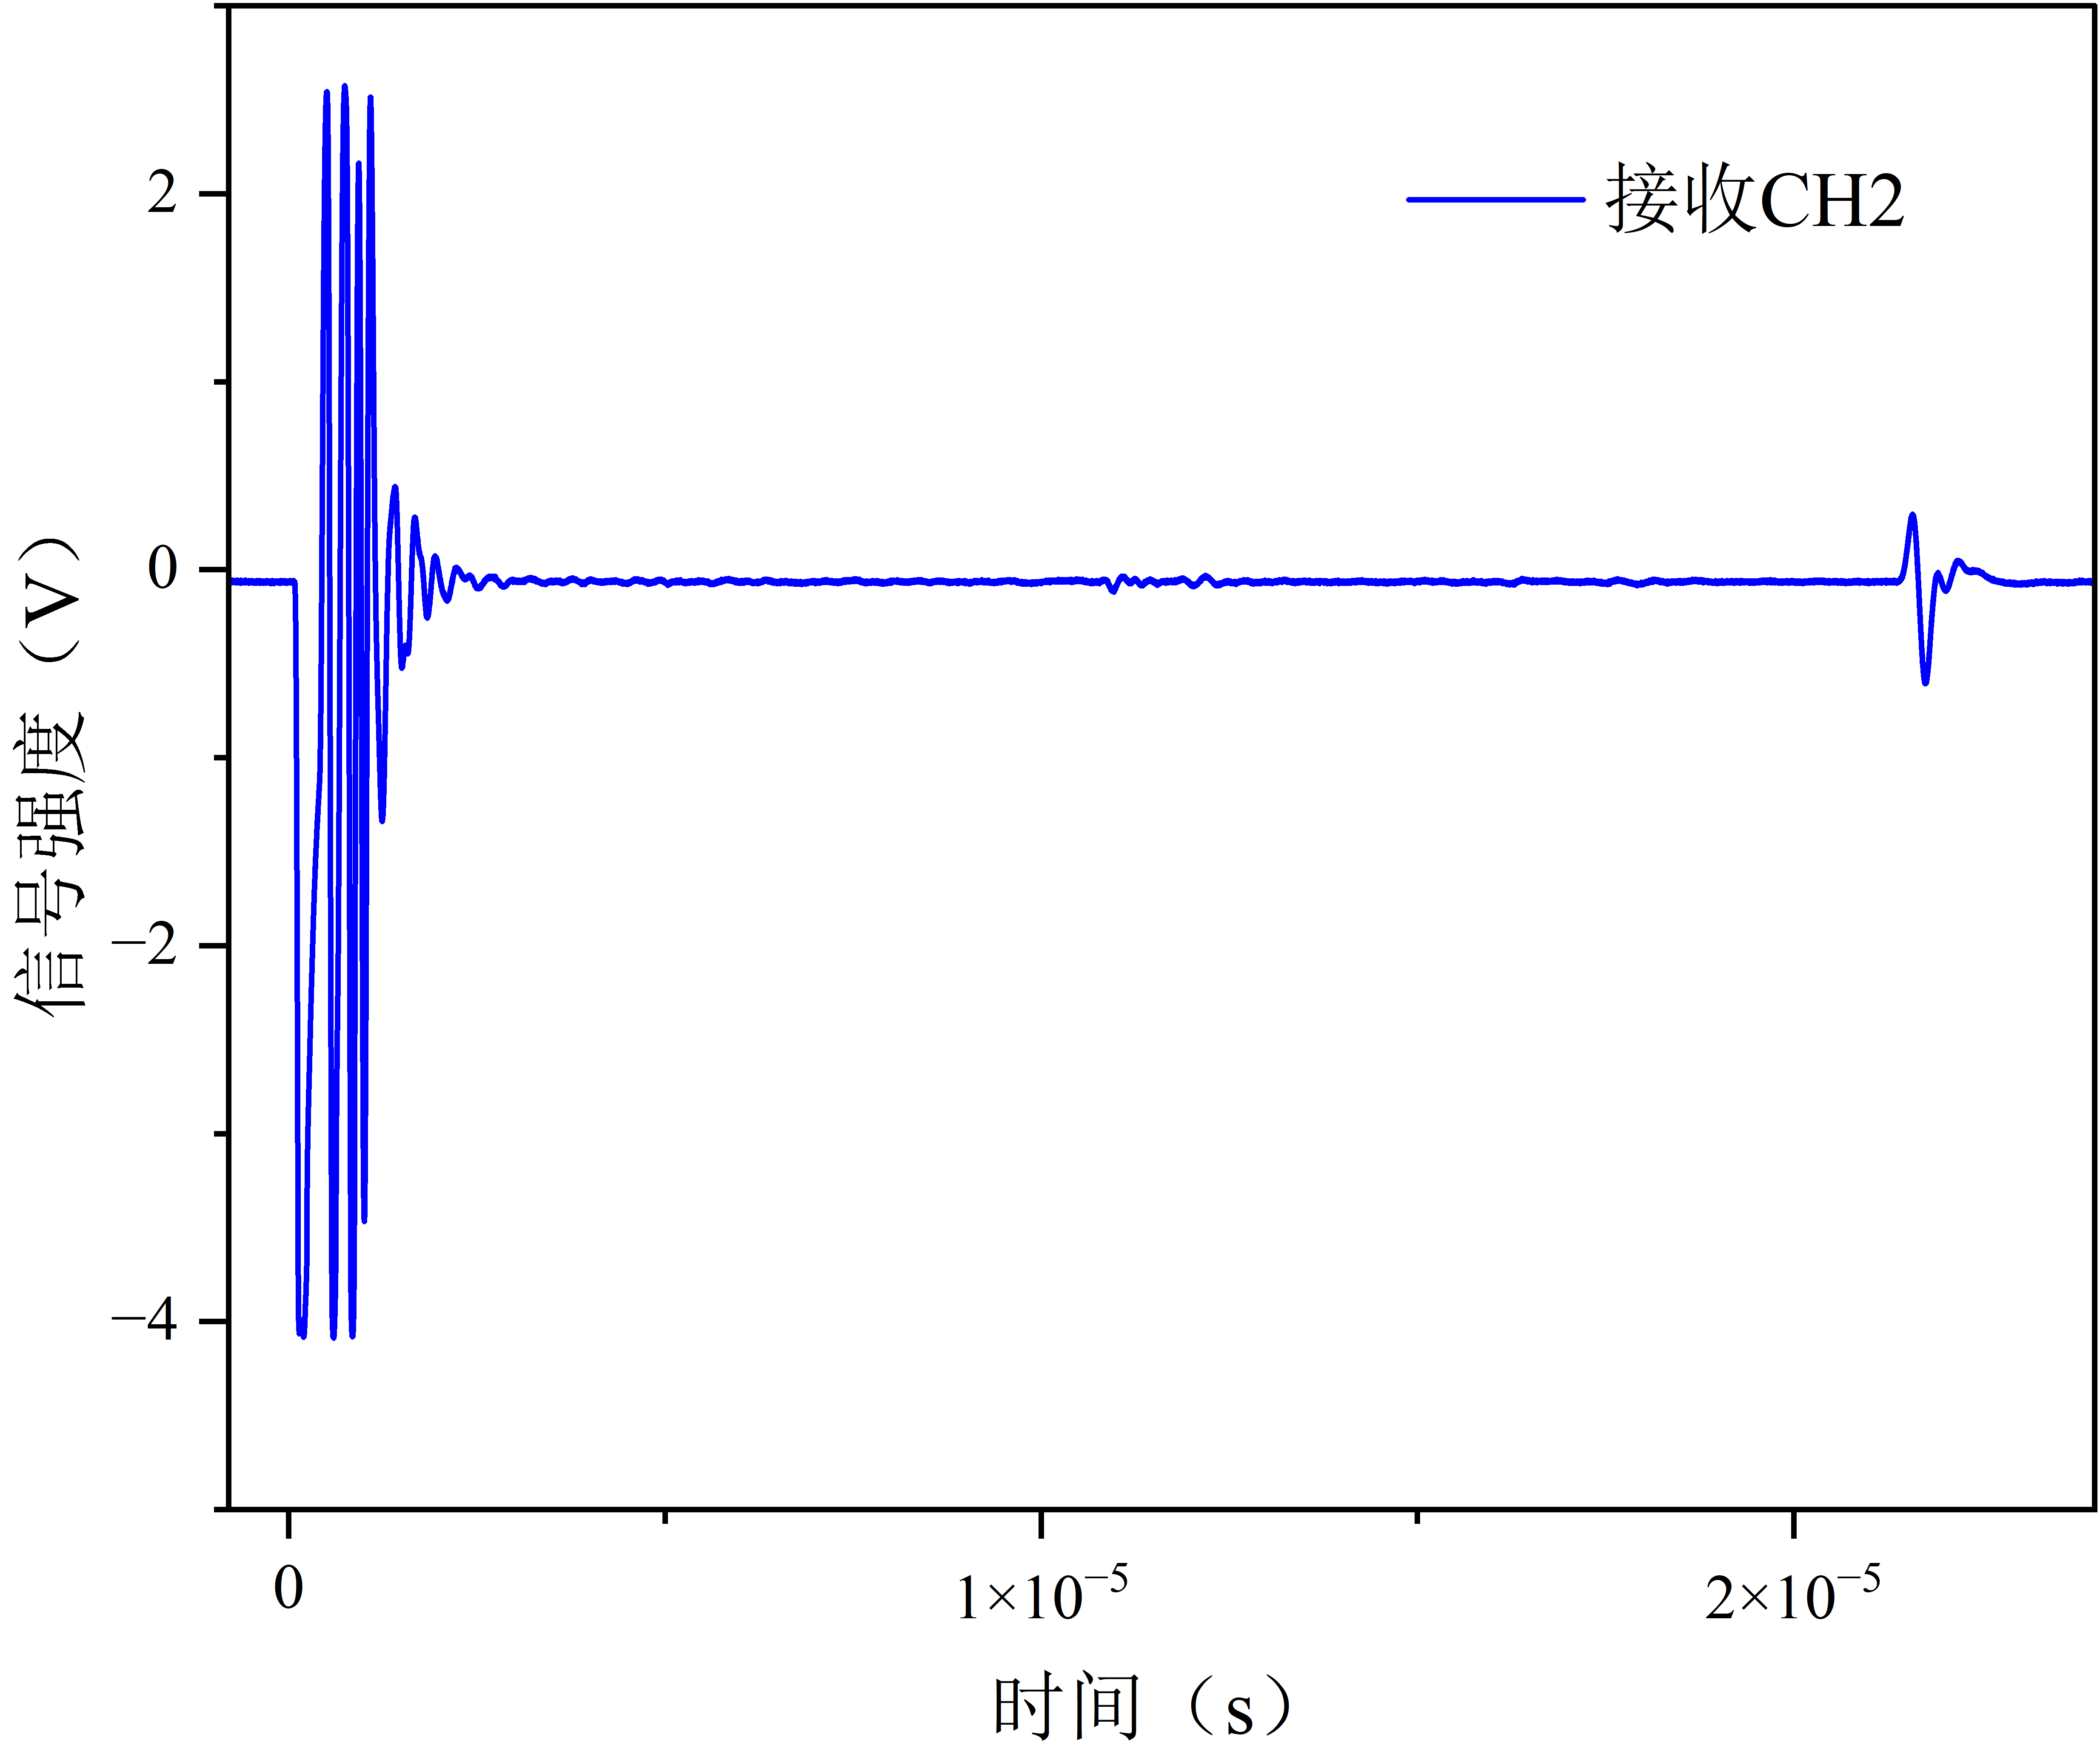
\includegraphics[width=\linewidth]{p13_img02.png}}
\caption{5 MHz 接触式测量有机玻璃试件横波波速时信号图}
\label{fig:exp2-og-S}
\end{figure}

\begin{table}[H]
\centering\scriptsize
\caption{5 MHz 接触式测量三种介质中横波波峰时间差}
\label{tab:exp2-S-time}
\setlength{\tabcolsep}{3pt}
\begin{tabular}{lccccccc}
\toprule
测量对象 & 测量1 & 测量2 & 测量3 & 均值 & $u_A$ & $u_B$ & $u$\\
\midrule
钢 $\Delta t$（$\mu$s） & \blank[0.8cm] & \blank[0.8cm] & \blank[0.8cm] & \blank[0.8cm] & \blank[0.9cm] & \blank[0.6cm] & \blank[0.9cm]\\
铝 $\Delta t$（$\mu$s） & \blank[0.8cm] & \blank[0.8cm] & \blank[0.8cm] & \blank[0.8cm] & \blank[0.9cm] & \blank[0.6cm] & \blank[0.9cm]\\
有机玻璃 $\Delta t$（$\mu$s） & \blank[0.8cm] & \blank[0.8cm] & \blank[0.8cm] & \blank[0.8cm] & \blank[0.9cm] & \blank[0.6cm] & \blank[0.9cm]\\
\bottomrule
\end{tabular}
\end{table}

三种介质中的横波波速为
\begin{subequations}
\begin{align}
  C_{S,st}&=\bar{C}_{S,st}\pm u(C_{S,st})=(\blank[1.4cm]\pm\blank[1.2cm])\ \mathrm{m/s},\\
  C_{S,al}&=\bar{C}_{S,al}\pm u(C_{S,al})=(\blank[1.4cm]\pm\blank[1.2cm])\ \mathrm{m/s},\\
  C_{S,og}&=\bar{C}_{S,og}\pm u(C_{S,og})=(\blank[1.4cm]\pm\blank[1.2cm])\ \mathrm{m/s}.
\end{align}
\end{subequations}
钢、铝和有机玻璃的横波波速参考值分别为 3230、3080 和 1300 m/s，相对误差为
\begin{subequations}
\begin{align}
  \Delta_{st}&=\frac{|C_{st}-C|}{C}\times100\%=\blank[1.8cm],\\
  \Delta_{al}&=\frac{|C_{al}-C|}{C}\times100\%=\blank[1.8cm],\\
  \Delta_{og}&=\frac{|C_{og}-C|}{C}\times100\%=\blank[1.8cm].
\end{align}
\end{subequations}
分析材料非均匀性、探头贴合程度、回波能量及增益设置对结果的影响。
\answer

\subsection{计算三种材料的材料常数}
根据前面测得的 5 MHz 纵波与横波波速，由公式\eqref{eq:exp2-E}计算材料常数。不确定度计算方式如下：
\begin{subequations}
\begin{align}
  u(\nu)&=\sqrt{\left(\frac{\partial\nu}{\partial C_S}\right)^2u^2(C_S)+
  \left(\frac{\partial\nu}{\partial C_L}\right)^2u^2(C_L)}\nonumber\\
  &=\frac{\bar{C}_L\bar{C}_S}{(\bar{C}_L^2-\bar{C}_S^2)^2}
  \sqrt{\bar{C}_L^2u^2(C_S)+\bar{C}_S^2u^2(C_L)},\\
  u(E)&=E\sqrt{\left[\frac{u(\rho)}{\bar{\rho}}\right]^2+
  \left[\frac{2u(C_S)}{\bar{C}_S}\right]^2+
  \left[\frac{u(\nu)}{1+\nu}\right]^2}.
\end{align}
\end{subequations}
代入本组数据得到
\begin{subequations}
\begin{align}
  \nu_{st}&=\blank[1.3cm]\pm\blank[1.2cm], &
  E_{st}&=(\blank[1.3cm]\pm\blank[1.2cm])\ \mathrm{GPa},\\
  \nu_{al}&=\blank[1.3cm]\pm\blank[1.2cm], &
  E_{al}&=(\blank[1.3cm]\pm\blank[1.2cm])\ \mathrm{GPa},\\
  \nu_{og}&=\blank[1.3cm]\pm\blank[1.2cm], &
  E_{og}&=(\blank[1.3cm]\pm\blank[1.2cm])\ \mathrm{GPa}.
\end{align}
\end{subequations}
参考资料：钢的弹性模量为 207 GPa、泊松比为 0.29；铝的弹性模量为 72 GPa、泊松比为 0.33；有机玻璃的弹性模量为 3.16 GPa、泊松比为 0.32。误差分别写为
\begin{subequations}
\begin{align}
  \Delta E_{st}&=\frac{|E_{st}-E|}{E}\times100\%=\blank[1.3cm], &
  \Delta\nu_{st}&=\frac{|\nu_{st}-\nu|}{\nu}\times100\%=\blank[1.3cm],\\
  \Delta E_{al}&=\frac{|E_{al}-E|}{E}\times100\%=\blank[1.3cm], &
  \Delta\nu_{al}&=\frac{|\nu_{al}-\nu|}{\nu}\times100\%=\blank[1.3cm],\\
  \Delta E_{og}&=\frac{|E_{og}-E|}{E}\times100\%=\blank[1.3cm], &
  \Delta\nu_{og}&=\frac{|\nu_{og}-\nu|}{\nu}\times100\%=\blank[1.3cm].
\end{align}
\end{subequations}
分析弹性模量和泊松比误差，尤其说明材料具体牌号或成分不明确可能造成的影响。
\answer

\section{不同频率探头测量钢、有机玻璃纵波波速及有机玻璃衰减系数}
\subsection{接触式测量钢和有机玻璃的纵波波速}
使用频率为 5 MHz 与 10 MHz 的纵波超声探头进行接触式测量，波形数据及用于计算波速的数据区域如图\ref{fig:exp2-steel-5}--图\ref{fig:exp2-og-10}所示，波峰时间差填入表\ref{tab:exp2-frequency-time}。

\begin{figure}[H]
\centering
\subcaptionbox{输入输出信号全局图}[0.48\textwidth]{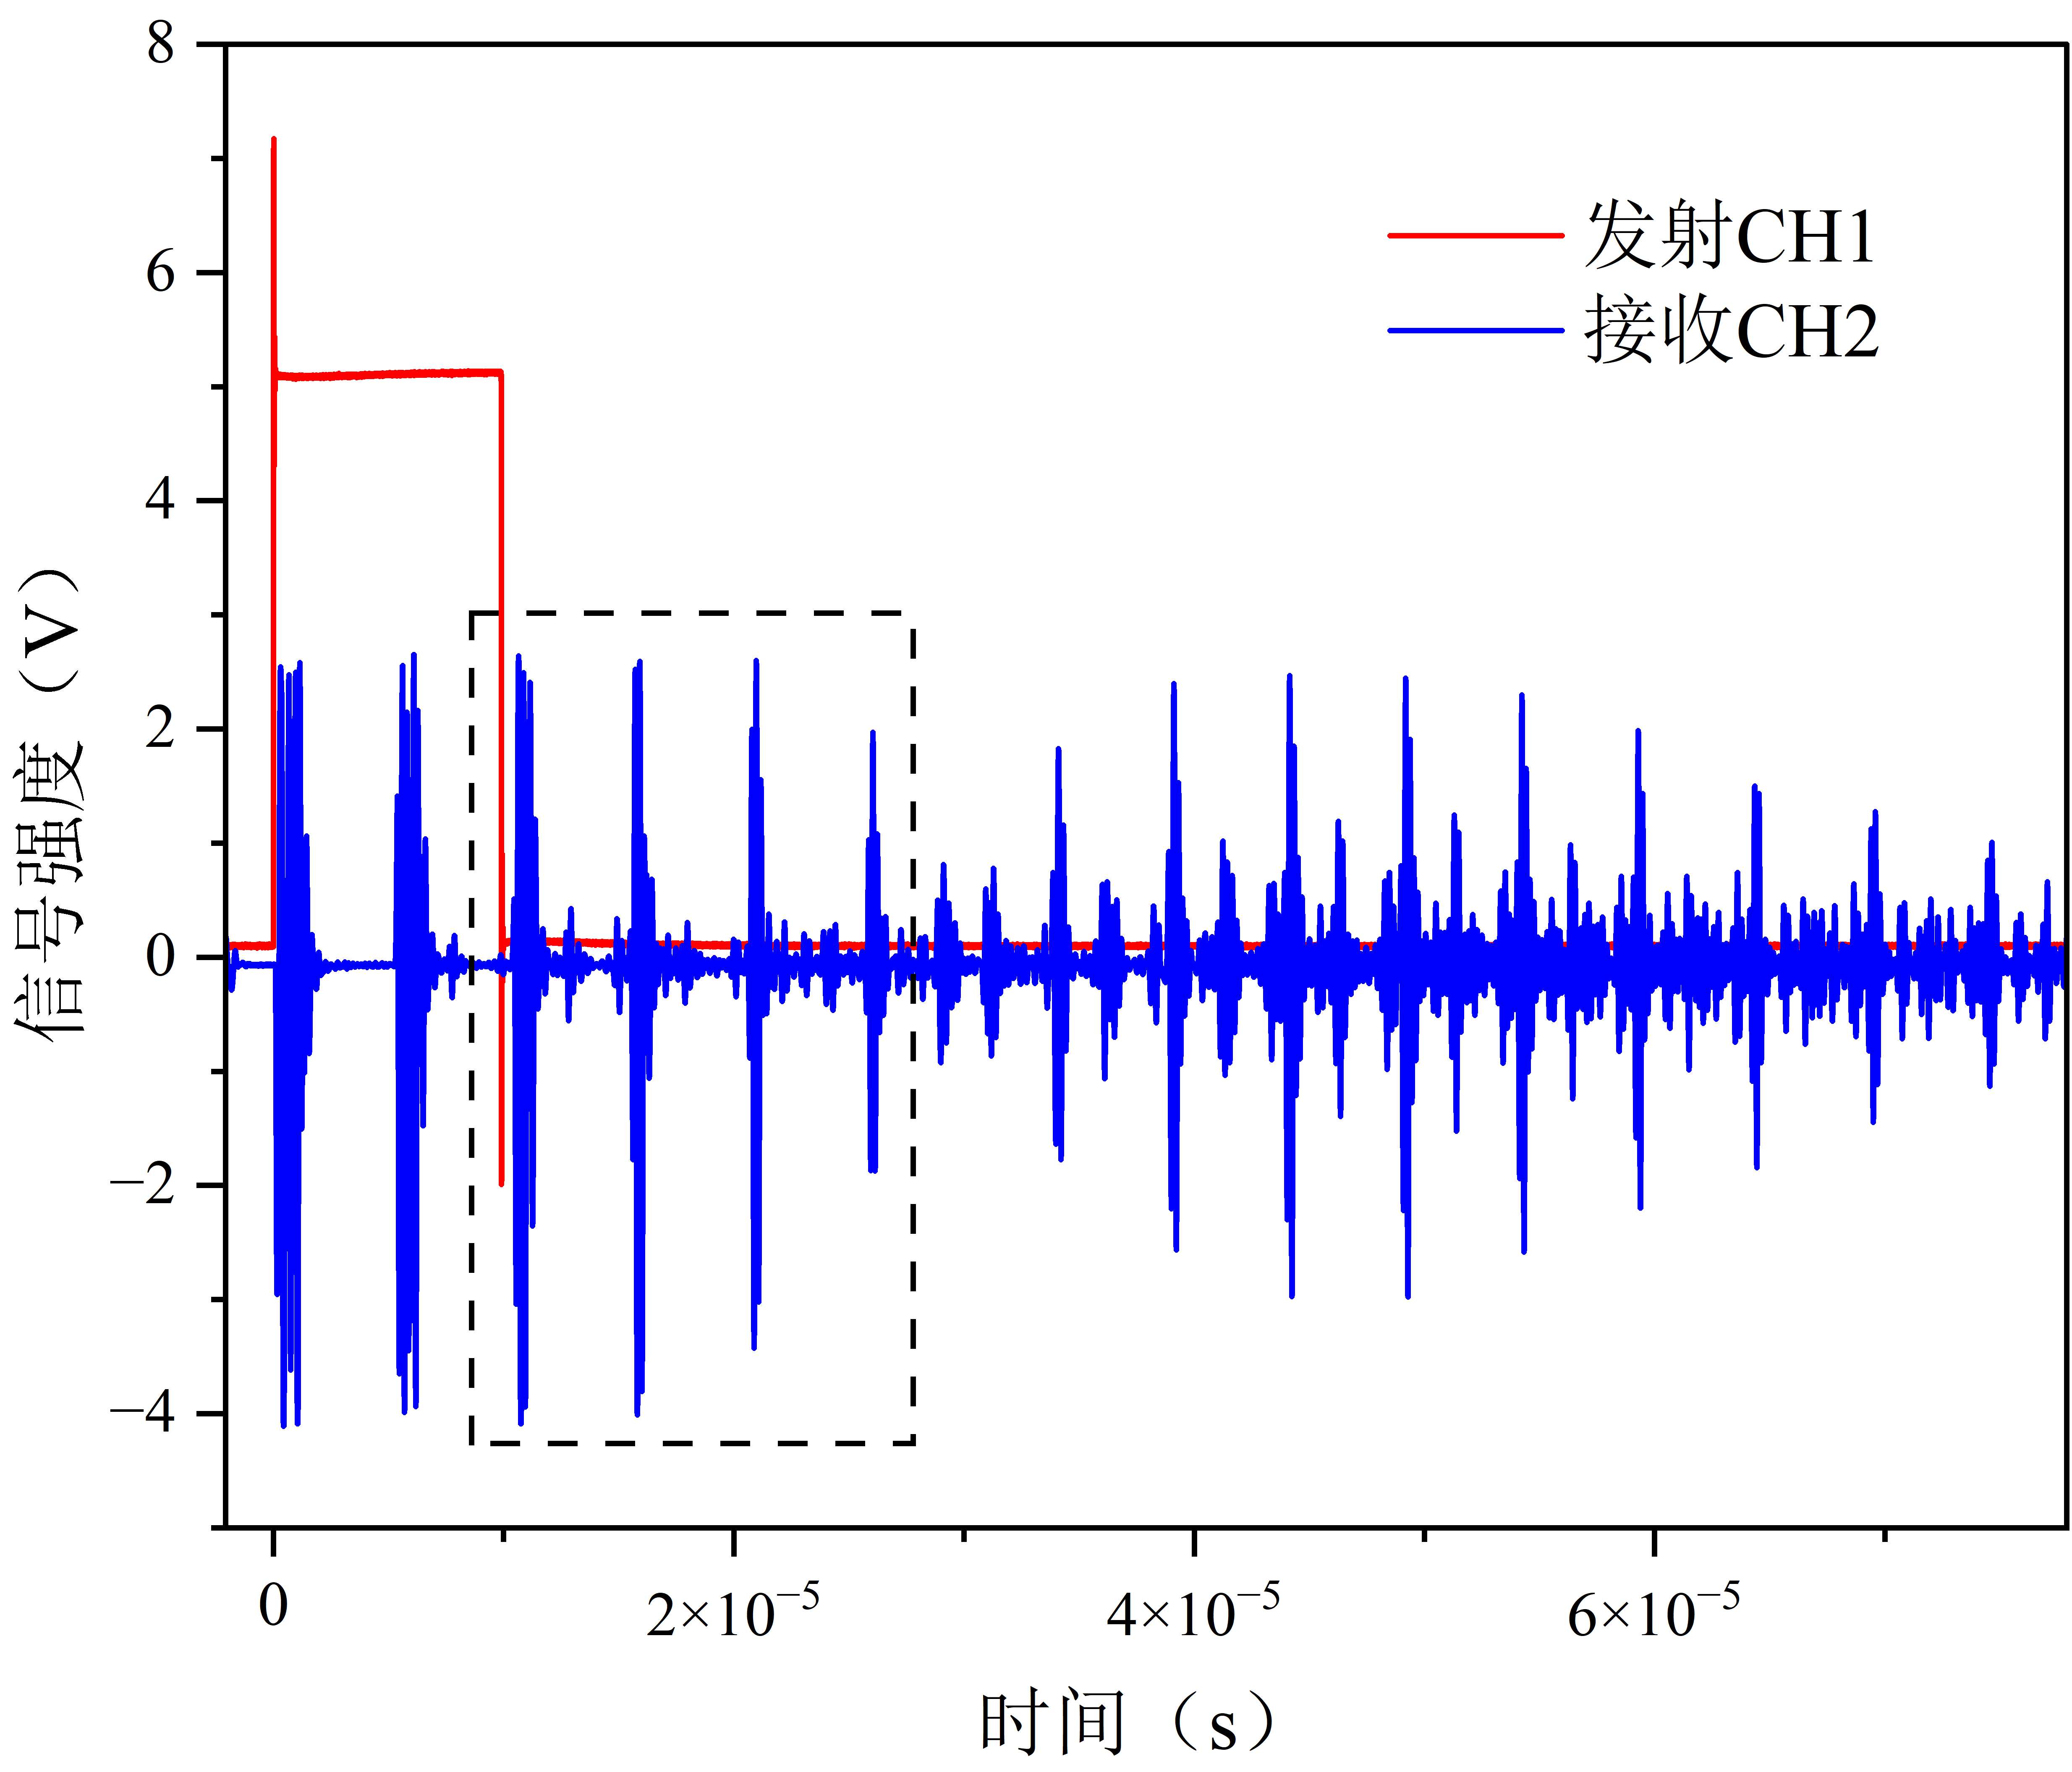
\includegraphics[width=\linewidth]{p14_img01.png}}\hfill
\subcaptionbox{输出信号局部放大图}[0.48\textwidth]{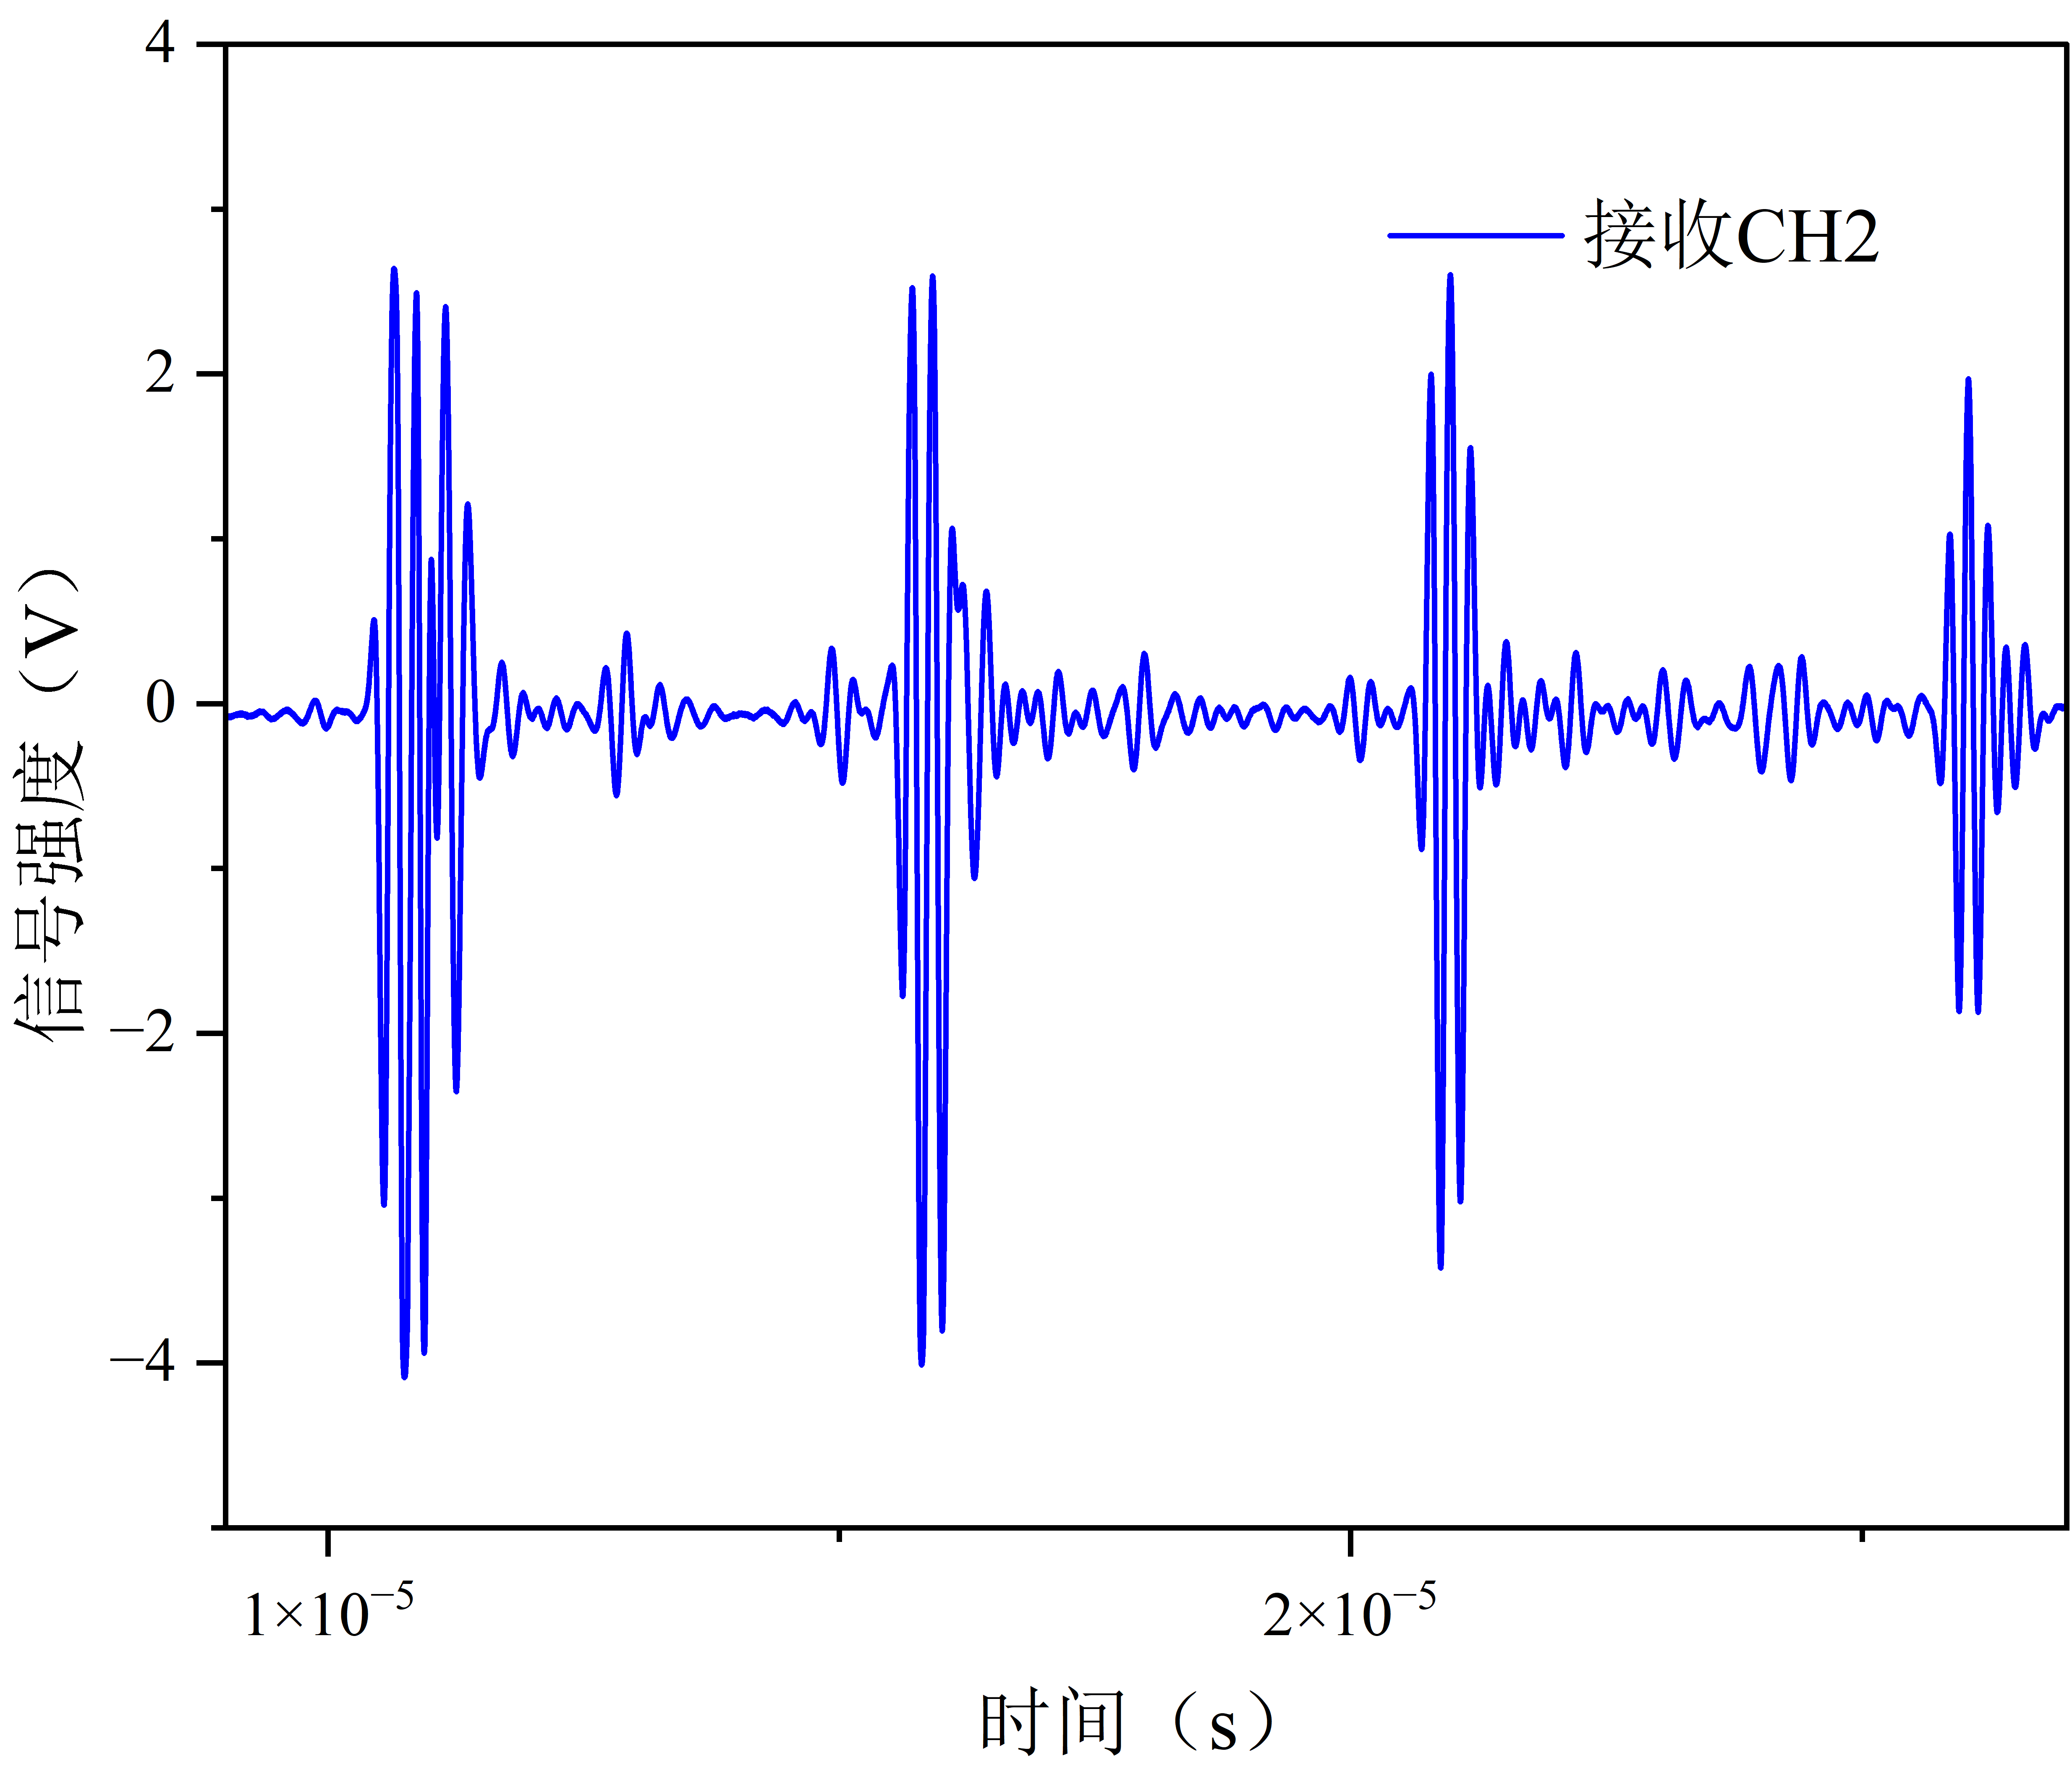
\includegraphics[width=\linewidth]{p14_img02.png}}
\caption{5 MHz 接触式测量钢试件纵波波速时信号图}
\label{fig:exp2-steel-5}
\end{figure}

\begin{figure}[H]
\centering
\subcaptionbox{输入输出信号全局图}[0.48\textwidth]{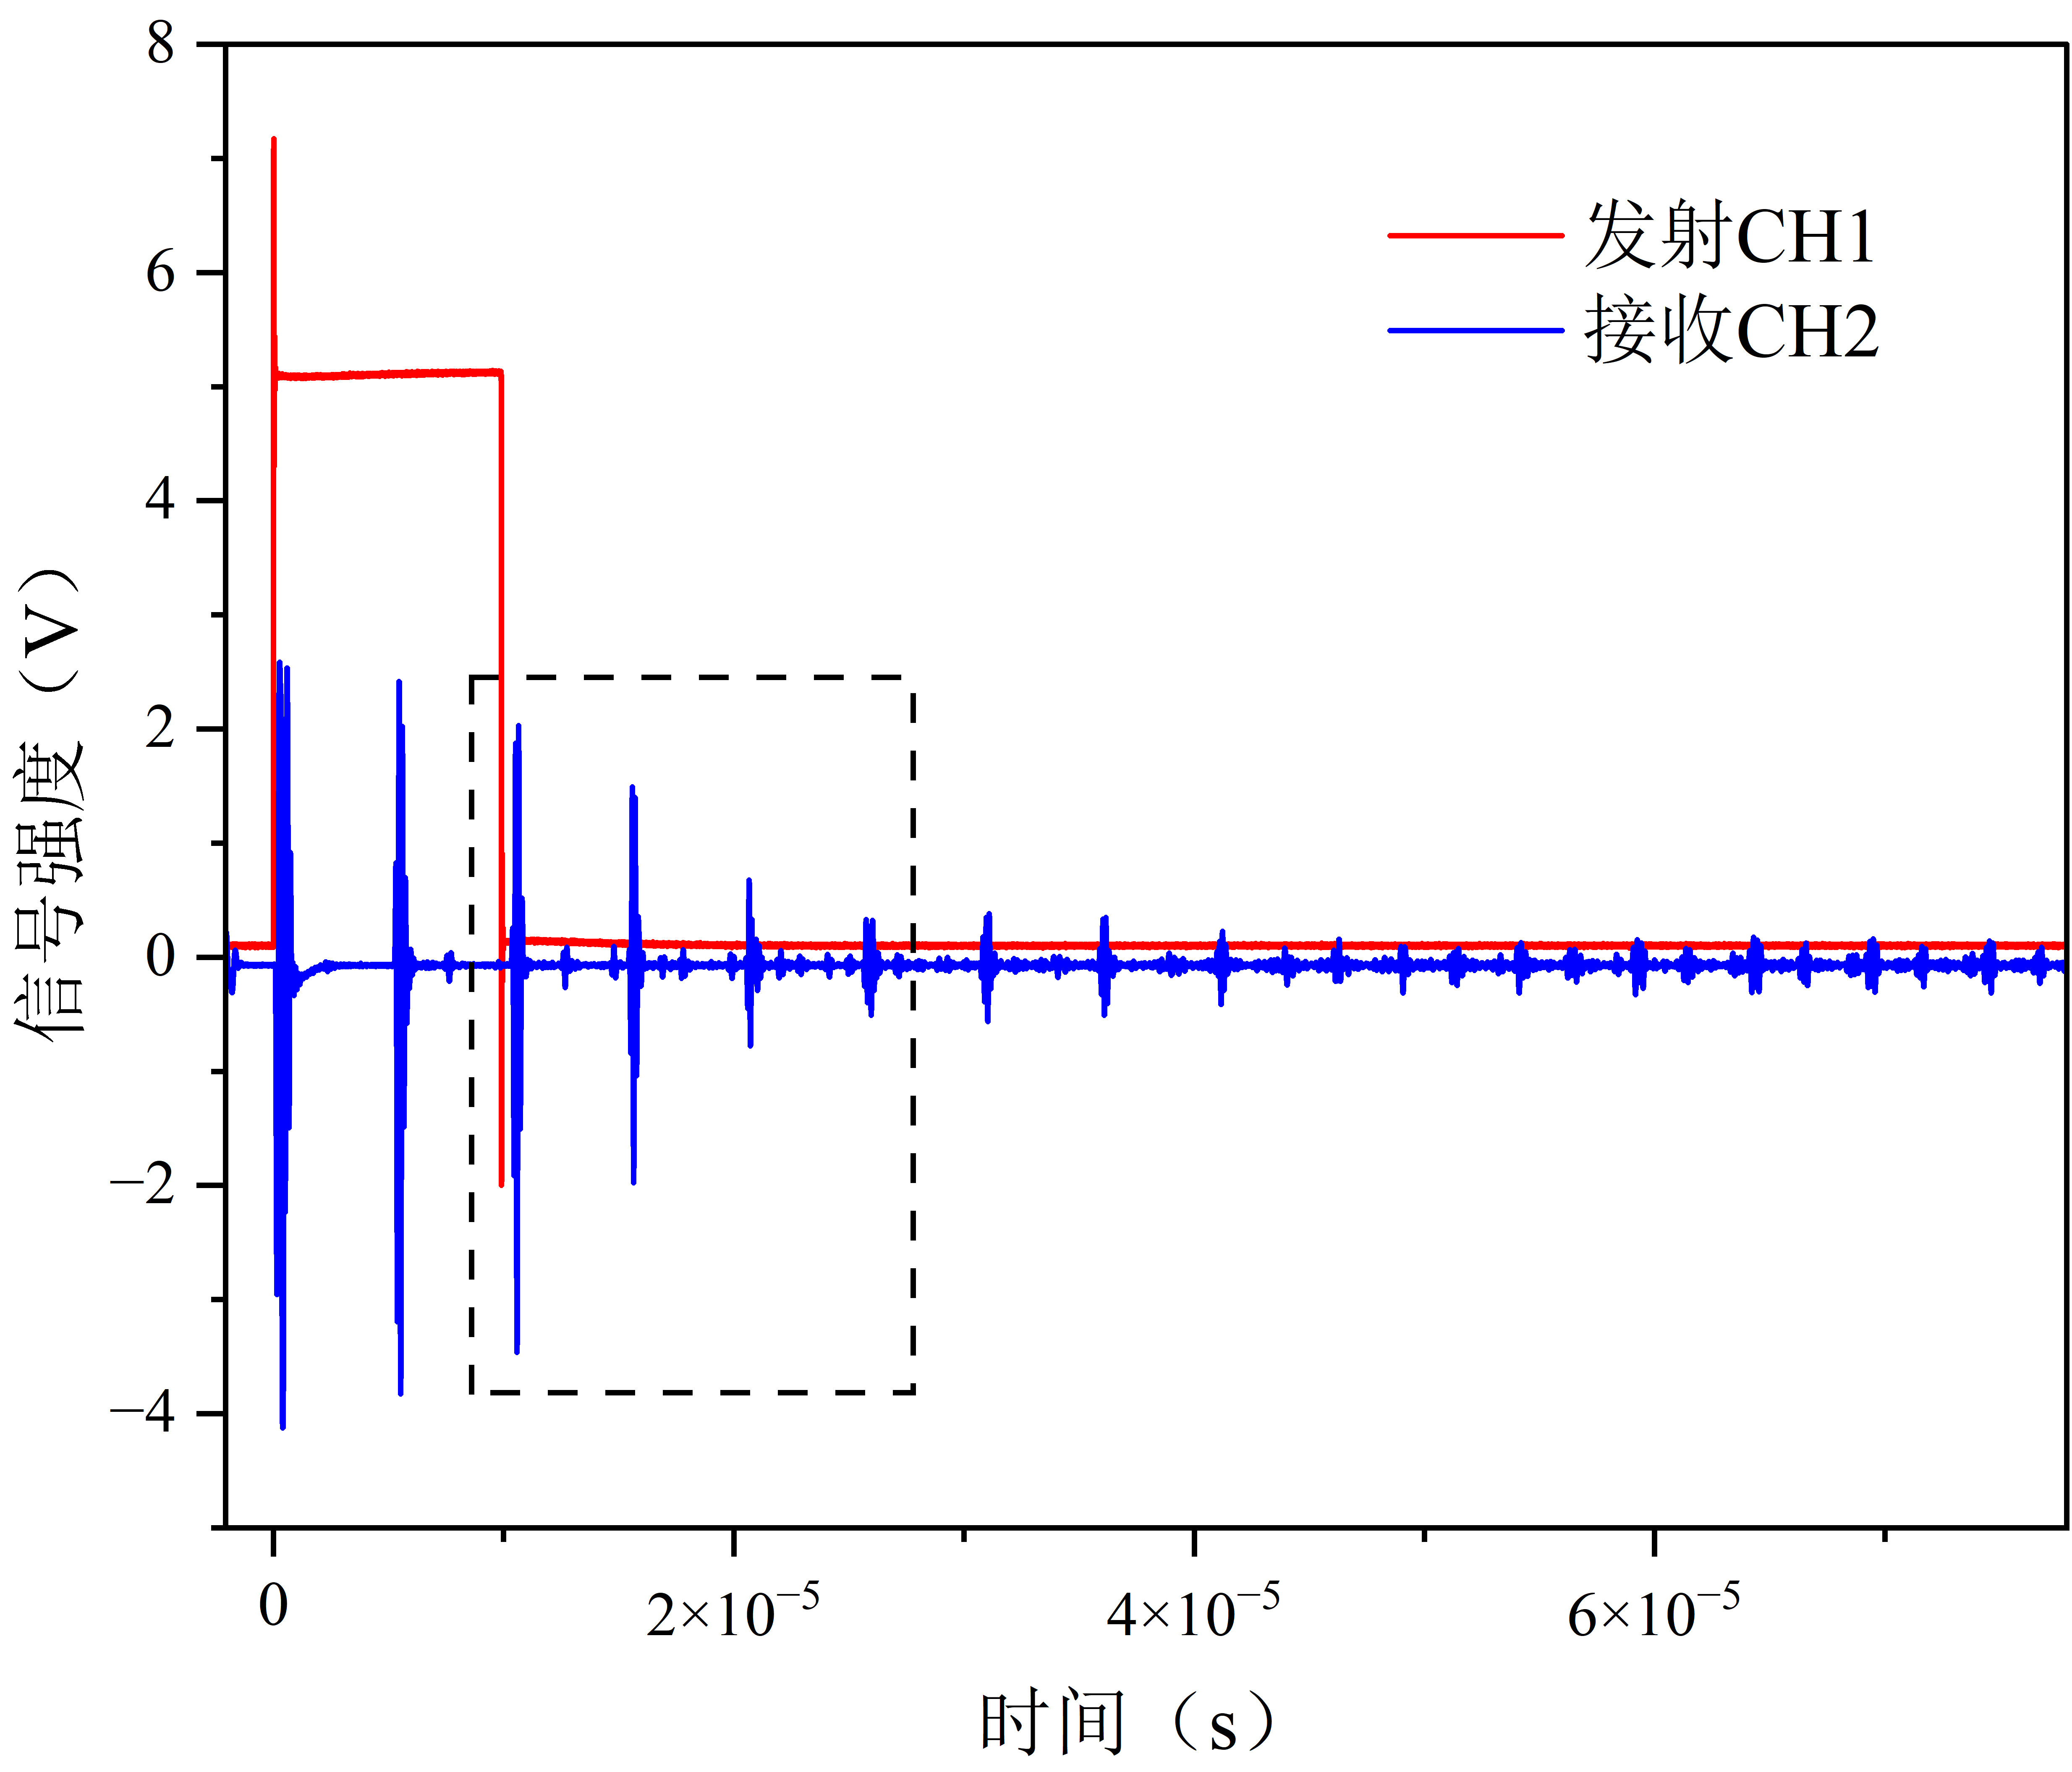
\includegraphics[width=\linewidth]{p14_img03.png}}\hfill
\subcaptionbox{输出信号局部放大图}[0.48\textwidth]{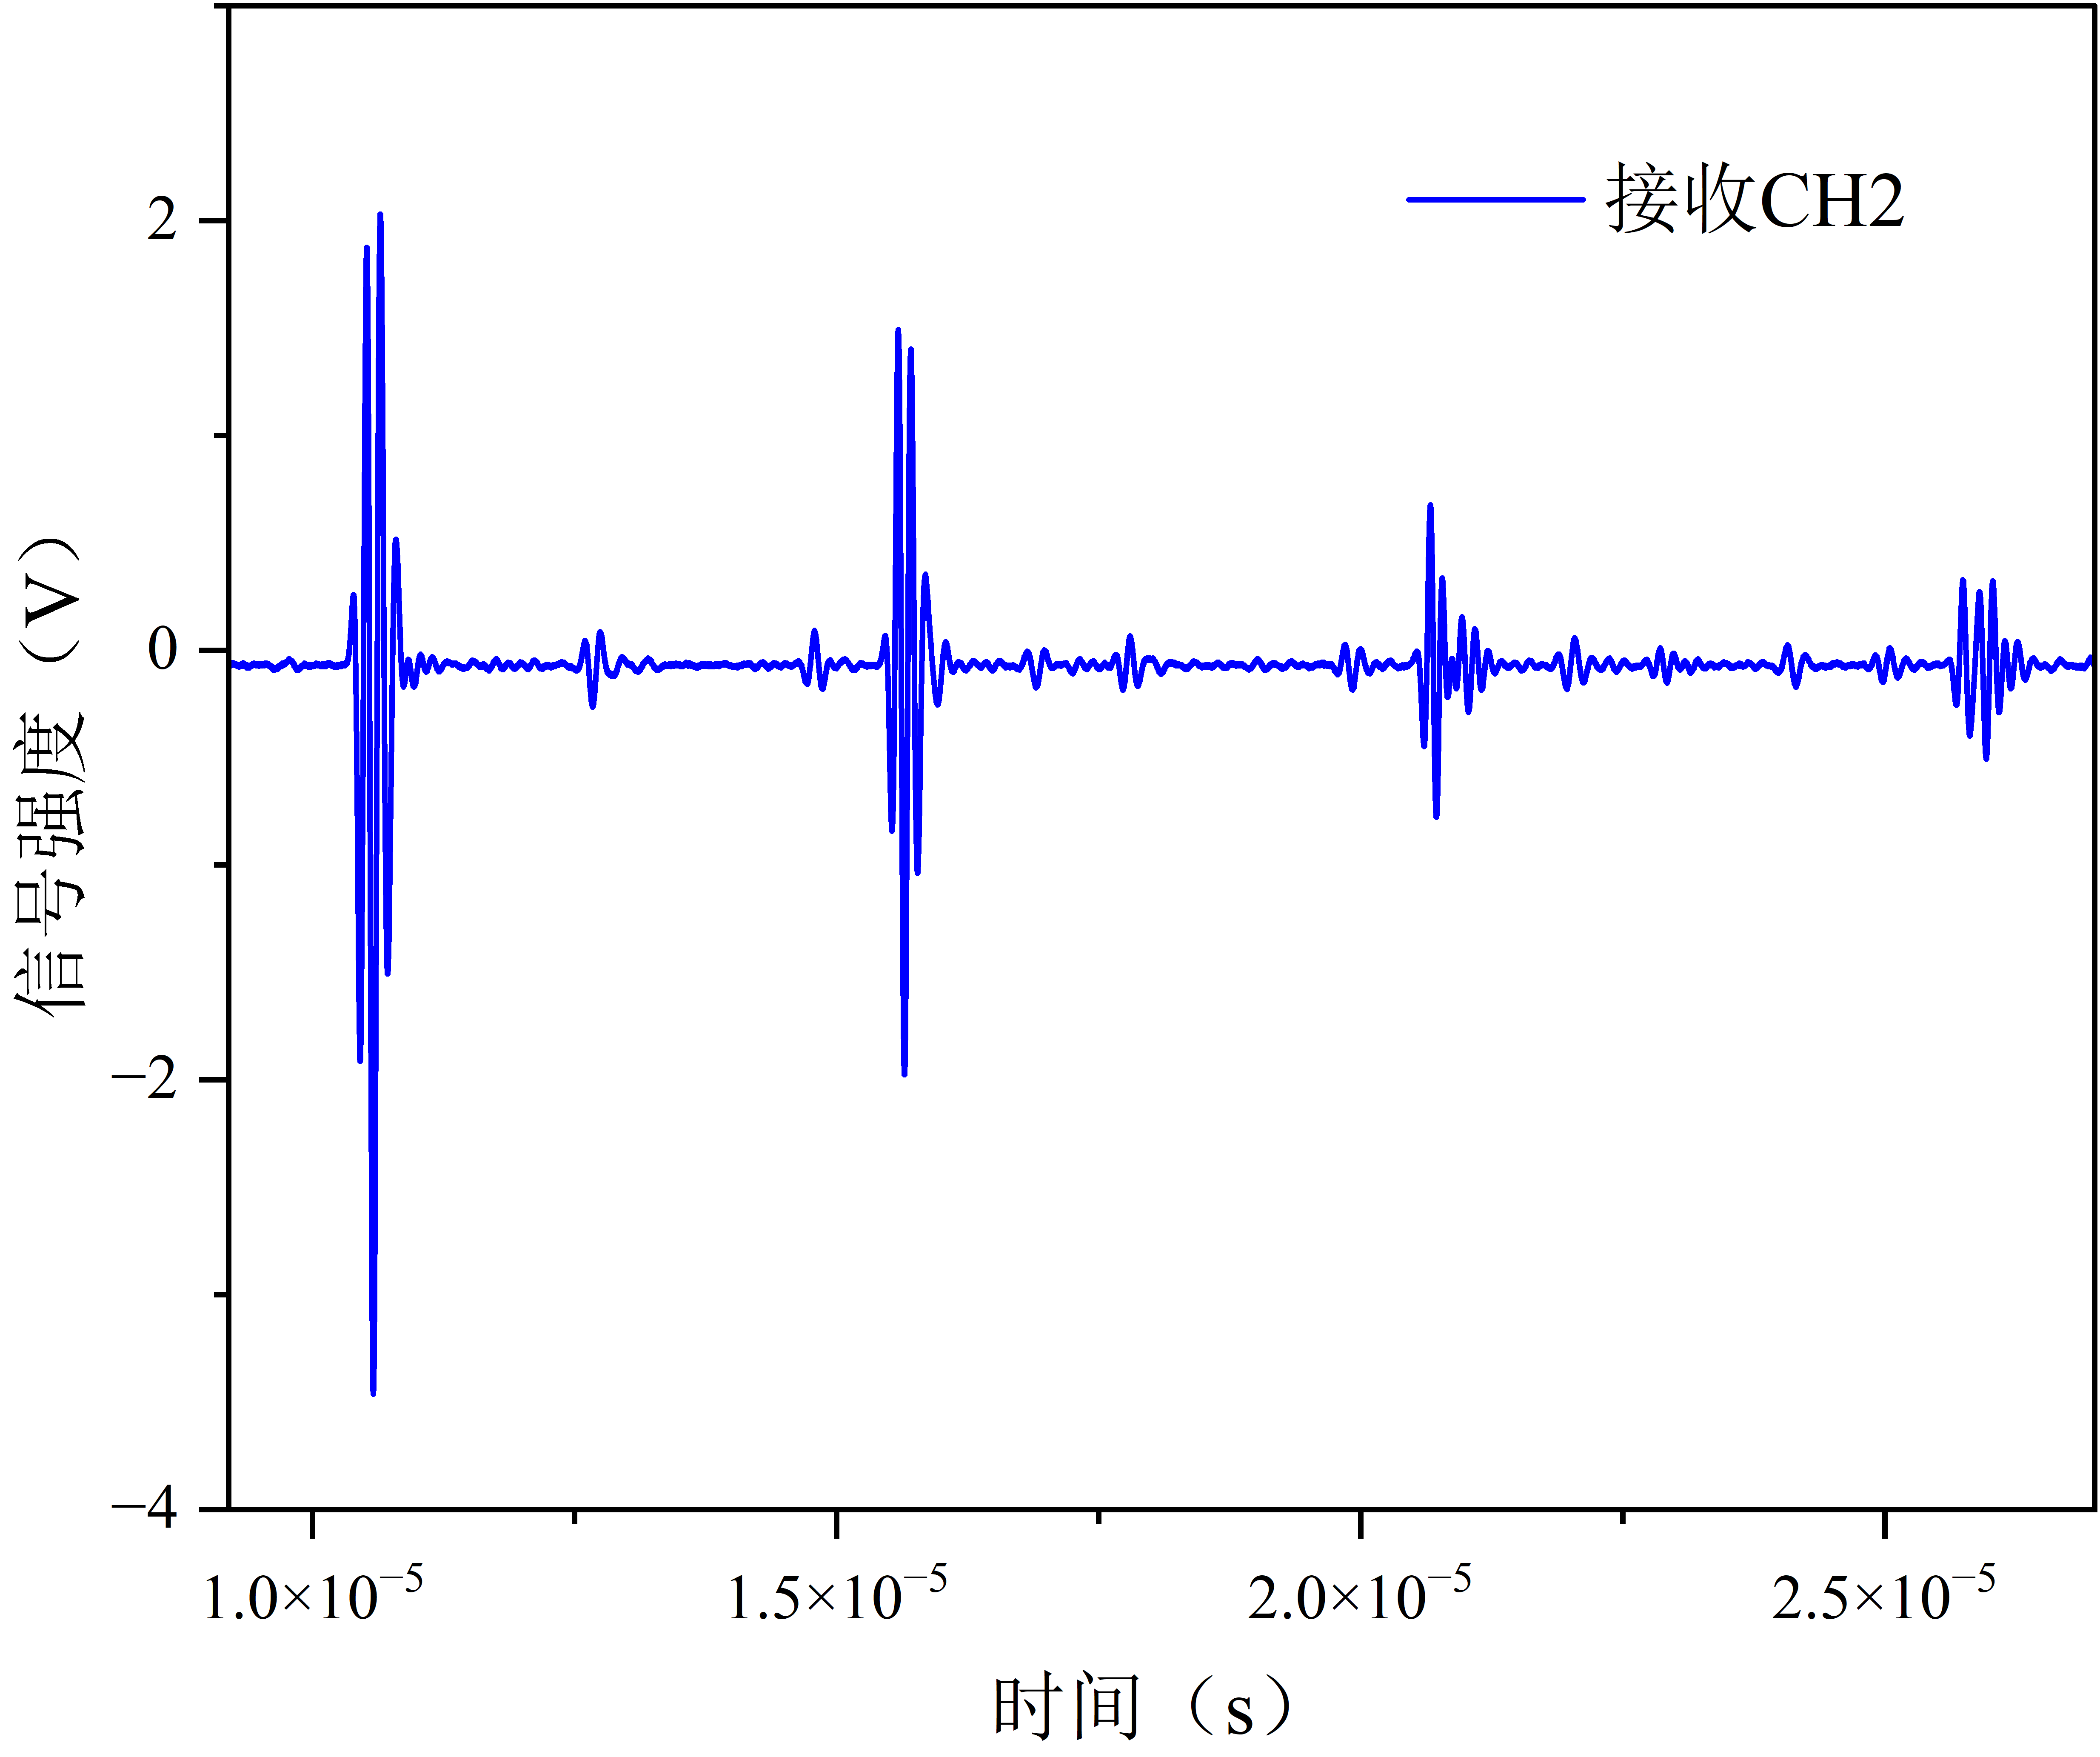
\includegraphics[width=\linewidth]{p14_img04.png}}
\caption{10 MHz 接触式测量钢试件纵波波速时信号图}
\end{figure}

\begin{figure}[H]
\centering
\subcaptionbox{输入输出信号全局图}[0.48\textwidth]{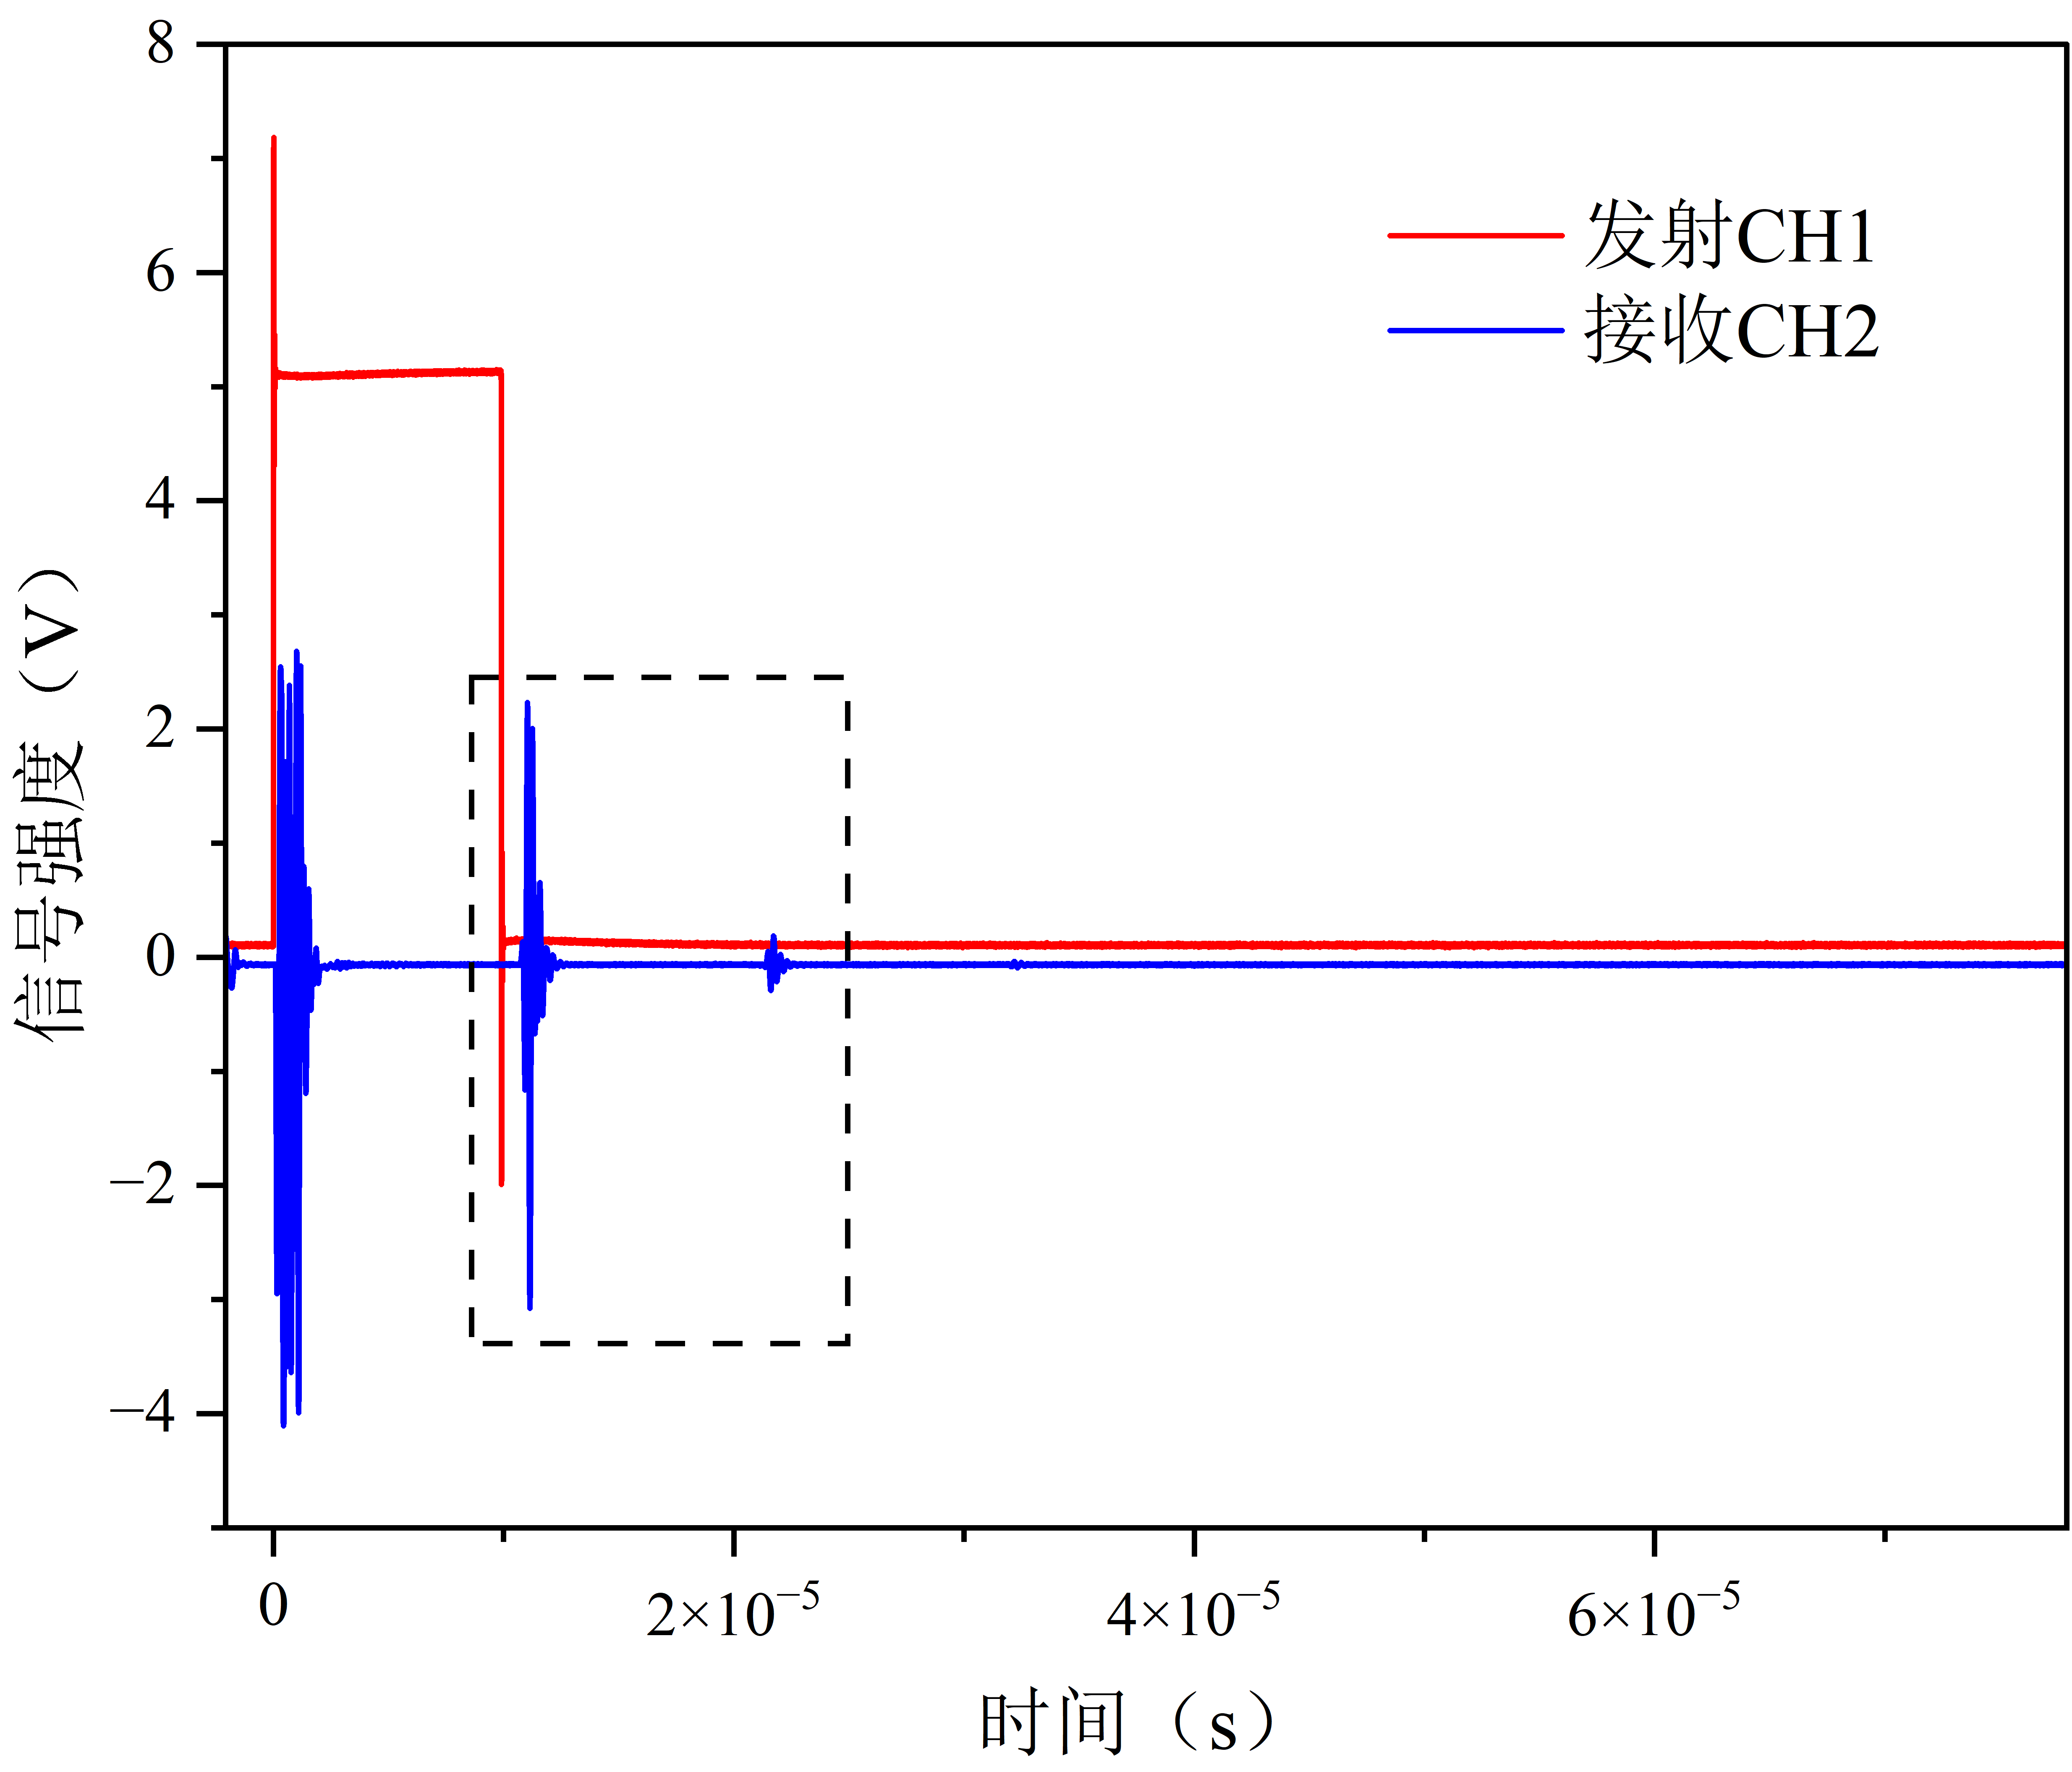
\includegraphics[width=\linewidth]{p15_img01.png}}\hfill
\subcaptionbox{输出信号局部放大图}[0.48\textwidth]{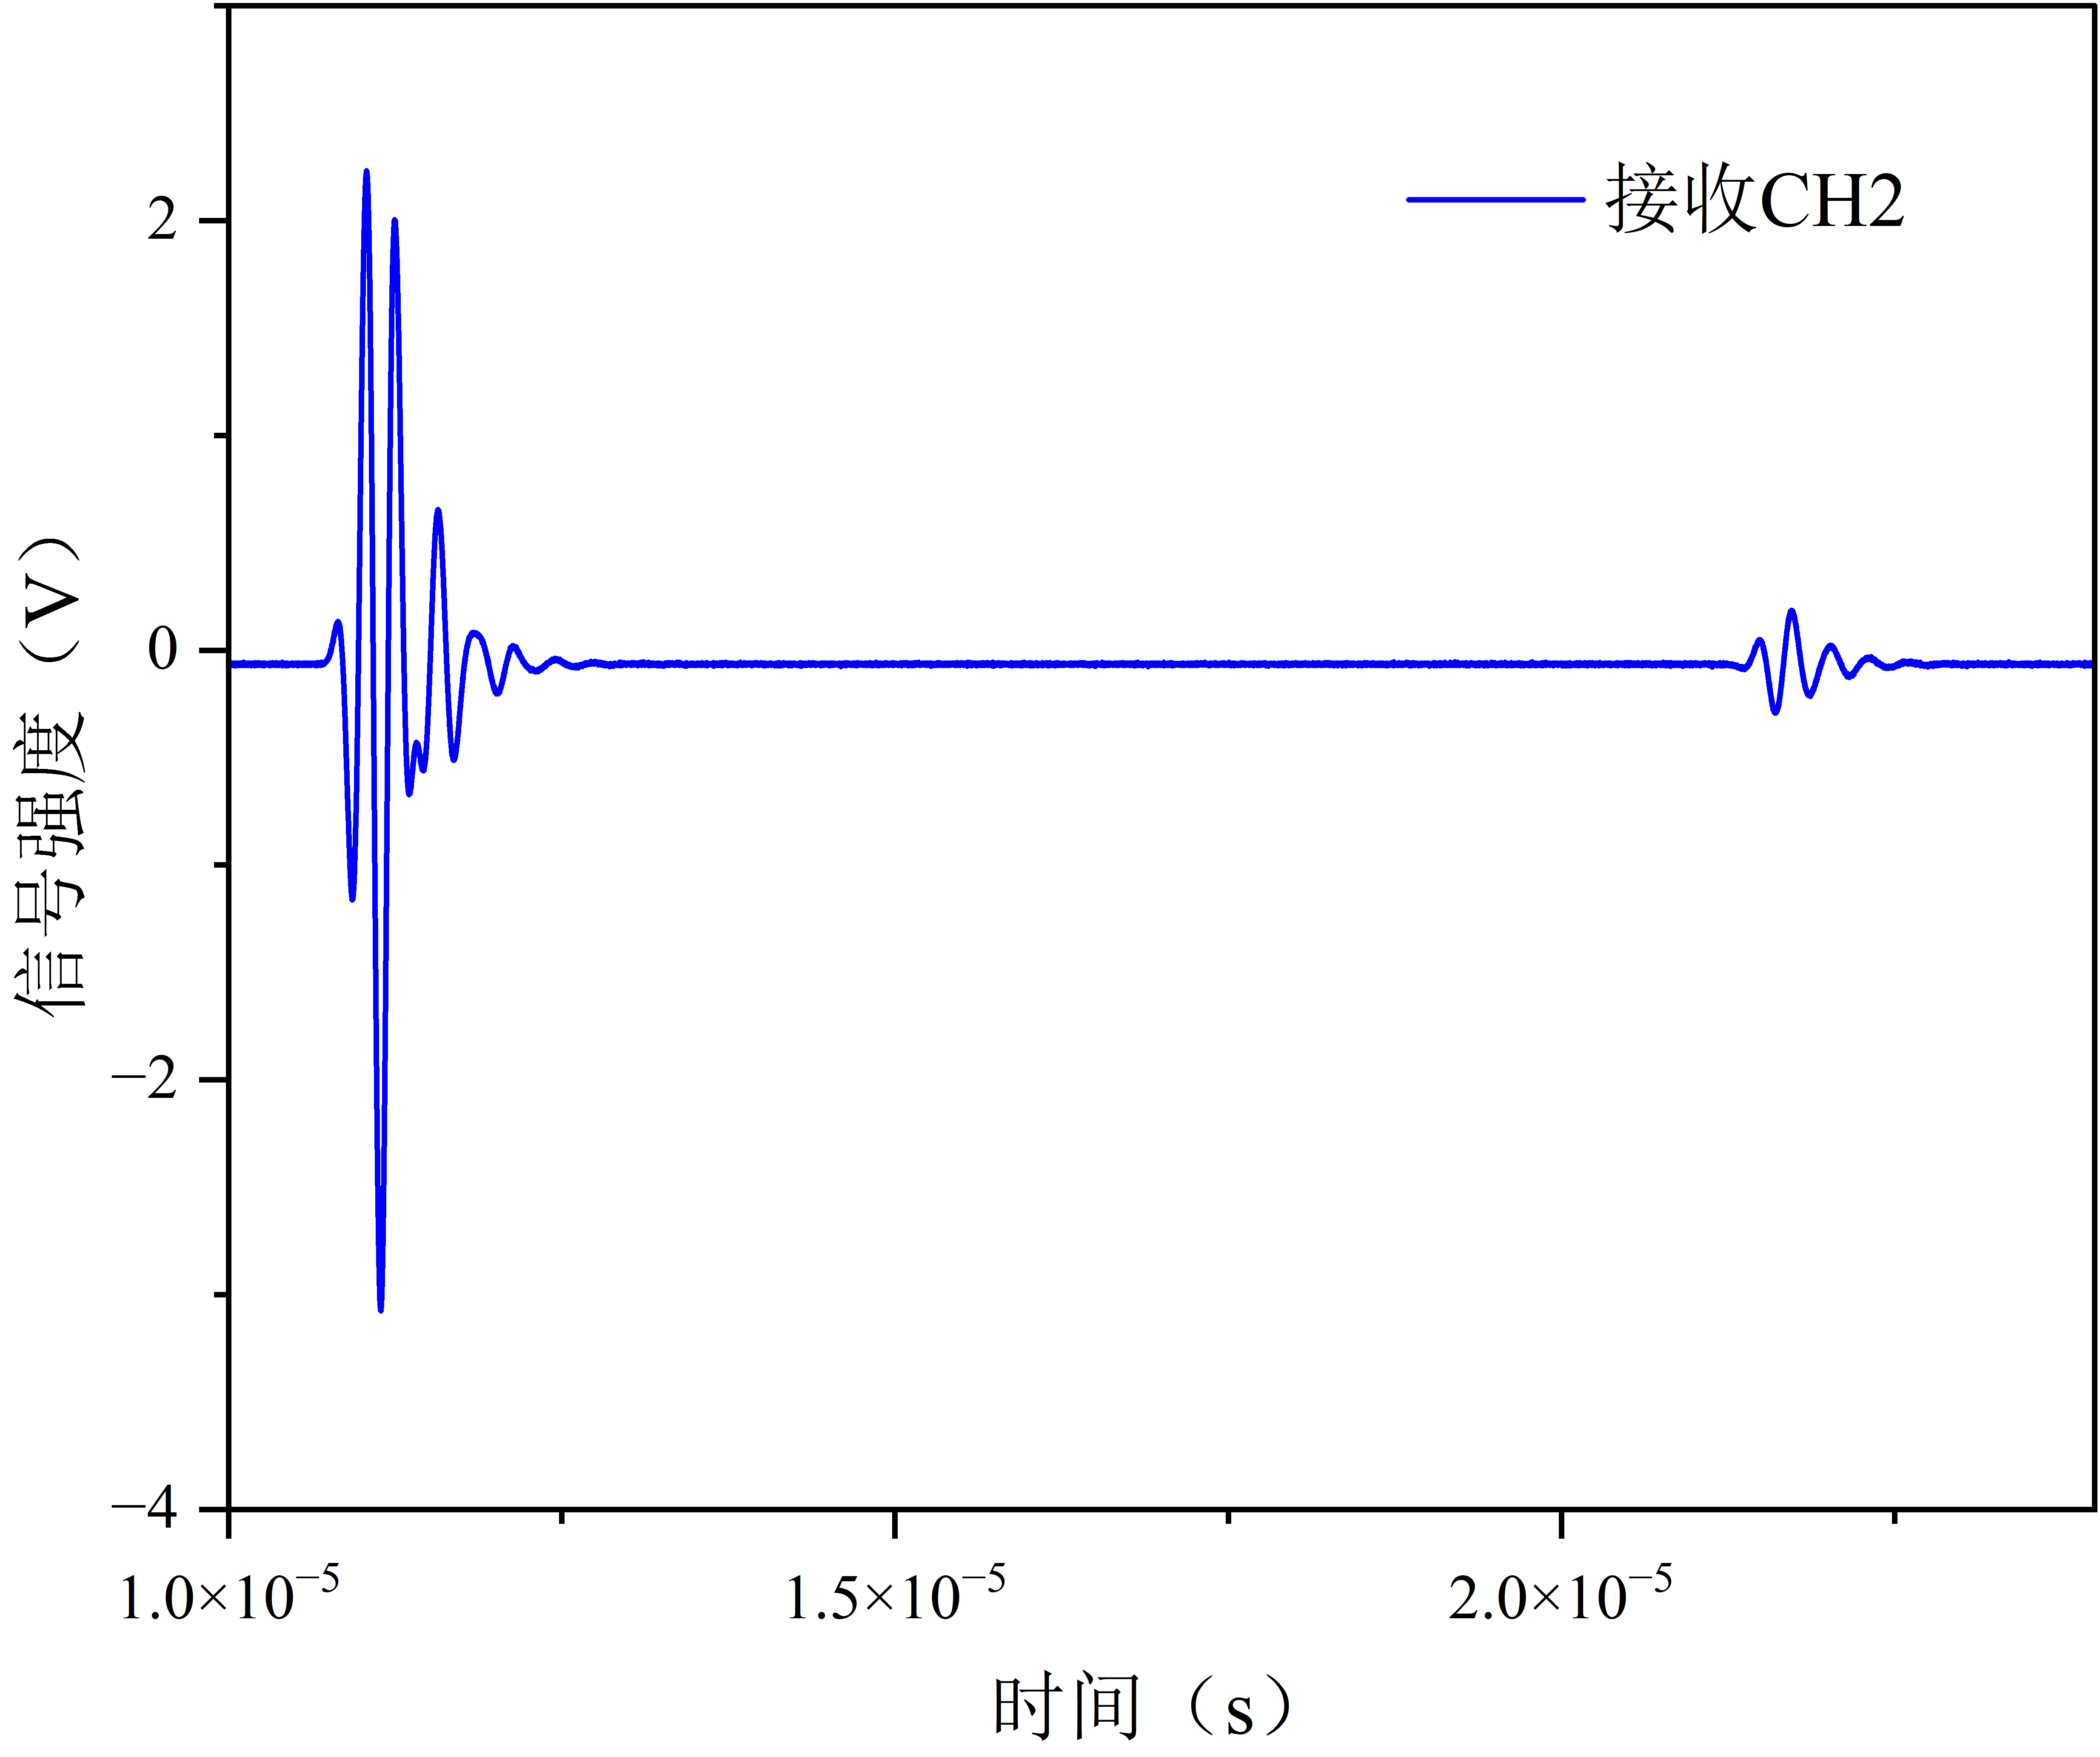
\includegraphics[width=\linewidth]{p15_img02.png}}
\caption{5 MHz 接触式测量有机玻璃试件纵波波速时信号图}
\label{fig:exp2-og-5}
\end{figure}

\begin{table}[H]
\centering\scriptsize
\caption{5 MHz 与 10 MHz 接触式测量钢和有机玻璃中纵波波峰时间差}
\label{tab:exp2-frequency-time}
\setlength{\tabcolsep}{2.5pt}
\begin{tabular}{llccccccc}
\toprule
测量对象 & 频率 & 测量1 & 测量2 & 测量3 & 均值 & $u_A$ & $u_B$ & $u$\\
\midrule
钢 $\Delta t$（$\mu$s） & 5 MHz & \blank[0.7cm] & \blank[0.7cm] & \blank[0.7cm] & \blank[0.7cm] & \blank[0.8cm] & \blank[0.5cm] & \blank[0.8cm]\\
钢 $\Delta t$（$\mu$s） & 10 MHz & \blank[0.7cm] & \blank[0.7cm] & \blank[0.7cm] & \blank[0.7cm] & \blank[0.8cm] & \blank[0.5cm] & \blank[0.8cm]\\
有机玻璃 $\Delta t$（$\mu$s） & 5 MHz & \blank[0.7cm] & \blank[0.7cm] & \blank[0.7cm] & \blank[0.7cm] & \blank[0.8cm] & \blank[0.5cm] & \blank[0.8cm]\\
有机玻璃 $\Delta t$（$\mu$s） & 10 MHz & \blank[0.7cm] & \blank[0.7cm] & \blank[0.7cm] & \blank[0.7cm] & \blank[0.8cm] & \blank[0.5cm] & \blank[0.8cm]\\
\bottomrule
\end{tabular}
\end{table}

计算得到 5 MHz 与 10 MHz 接触式测量钢和有机玻璃中纵波的波速：
\begin{subequations}
\begin{align}
  C_{L,st}^{5\mathrm{MHz}}&=(\blank[1.4cm]\pm\blank[1.1cm])\ \mathrm{m/s}, &
  C_{L,st}^{10\mathrm{MHz}}&=(\blank[1.4cm]\pm\blank[1.1cm])\ \mathrm{m/s},\\
  C_{L,og}^{5\mathrm{MHz}}&=(\blank[1.4cm]\pm\blank[1.1cm])\ \mathrm{m/s}, &
  C_{L,og}^{10\mathrm{MHz}}&=(\blank[1.4cm]\pm\blank[1.1cm])\ \mathrm{m/s}.
\end{align}
\end{subequations}
将本结果与水浸法测量结果比较，分析测量方法及探头频率对波速、杂波和测量精度的影响。
\answer

\subsection{接触式测量有机玻璃纵波的衰减系数}
利用试件上下表面反射波振幅的关系，可以得到纵波在有机玻璃中的衰减系数。基于图\ref{fig:exp2-og-5}和图\ref{fig:exp2-og-10}读取不同时间下的波峰数值，将数据代入公式\eqref{eq:exp2-attenuation}，结果填入表\ref{tab:exp2-frequency-attenuation}。

\begin{figure}[H]
\centering
\subcaptionbox{输入输出信号全局图}[0.48\textwidth]{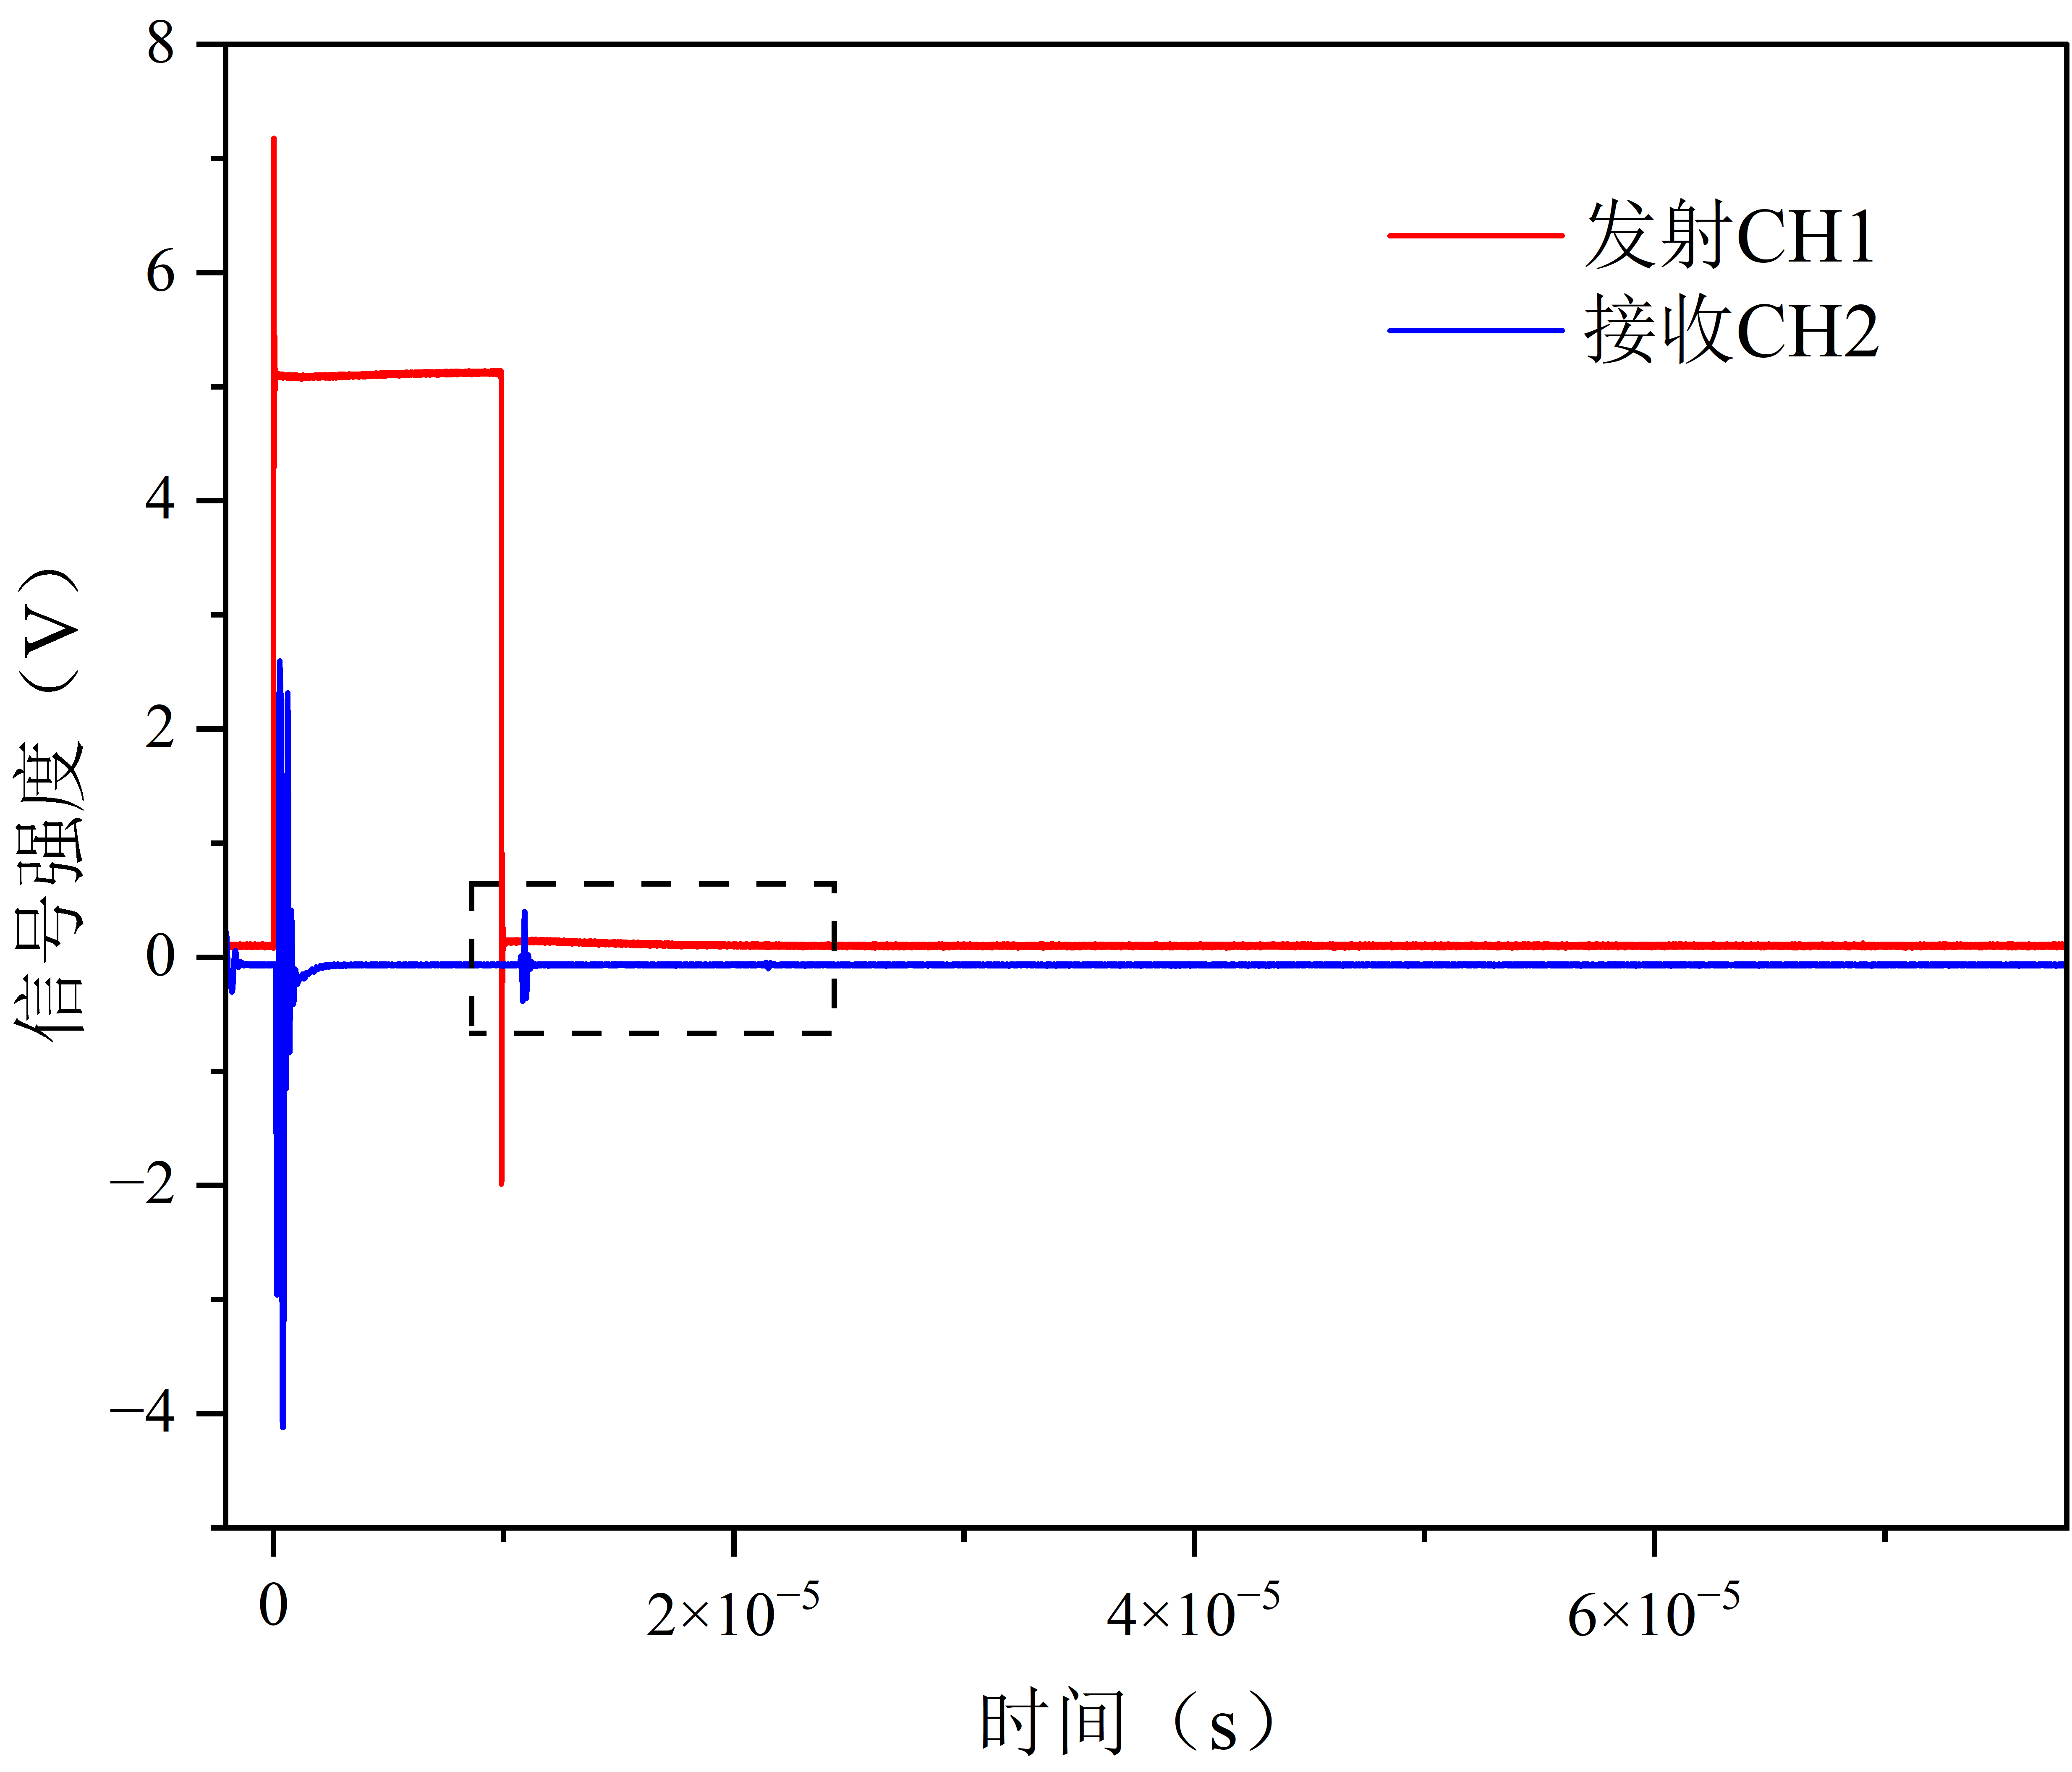
\includegraphics[width=\linewidth]{p16_img01.png}}\hfill
\subcaptionbox{输出信号局部放大图}[0.48\textwidth]{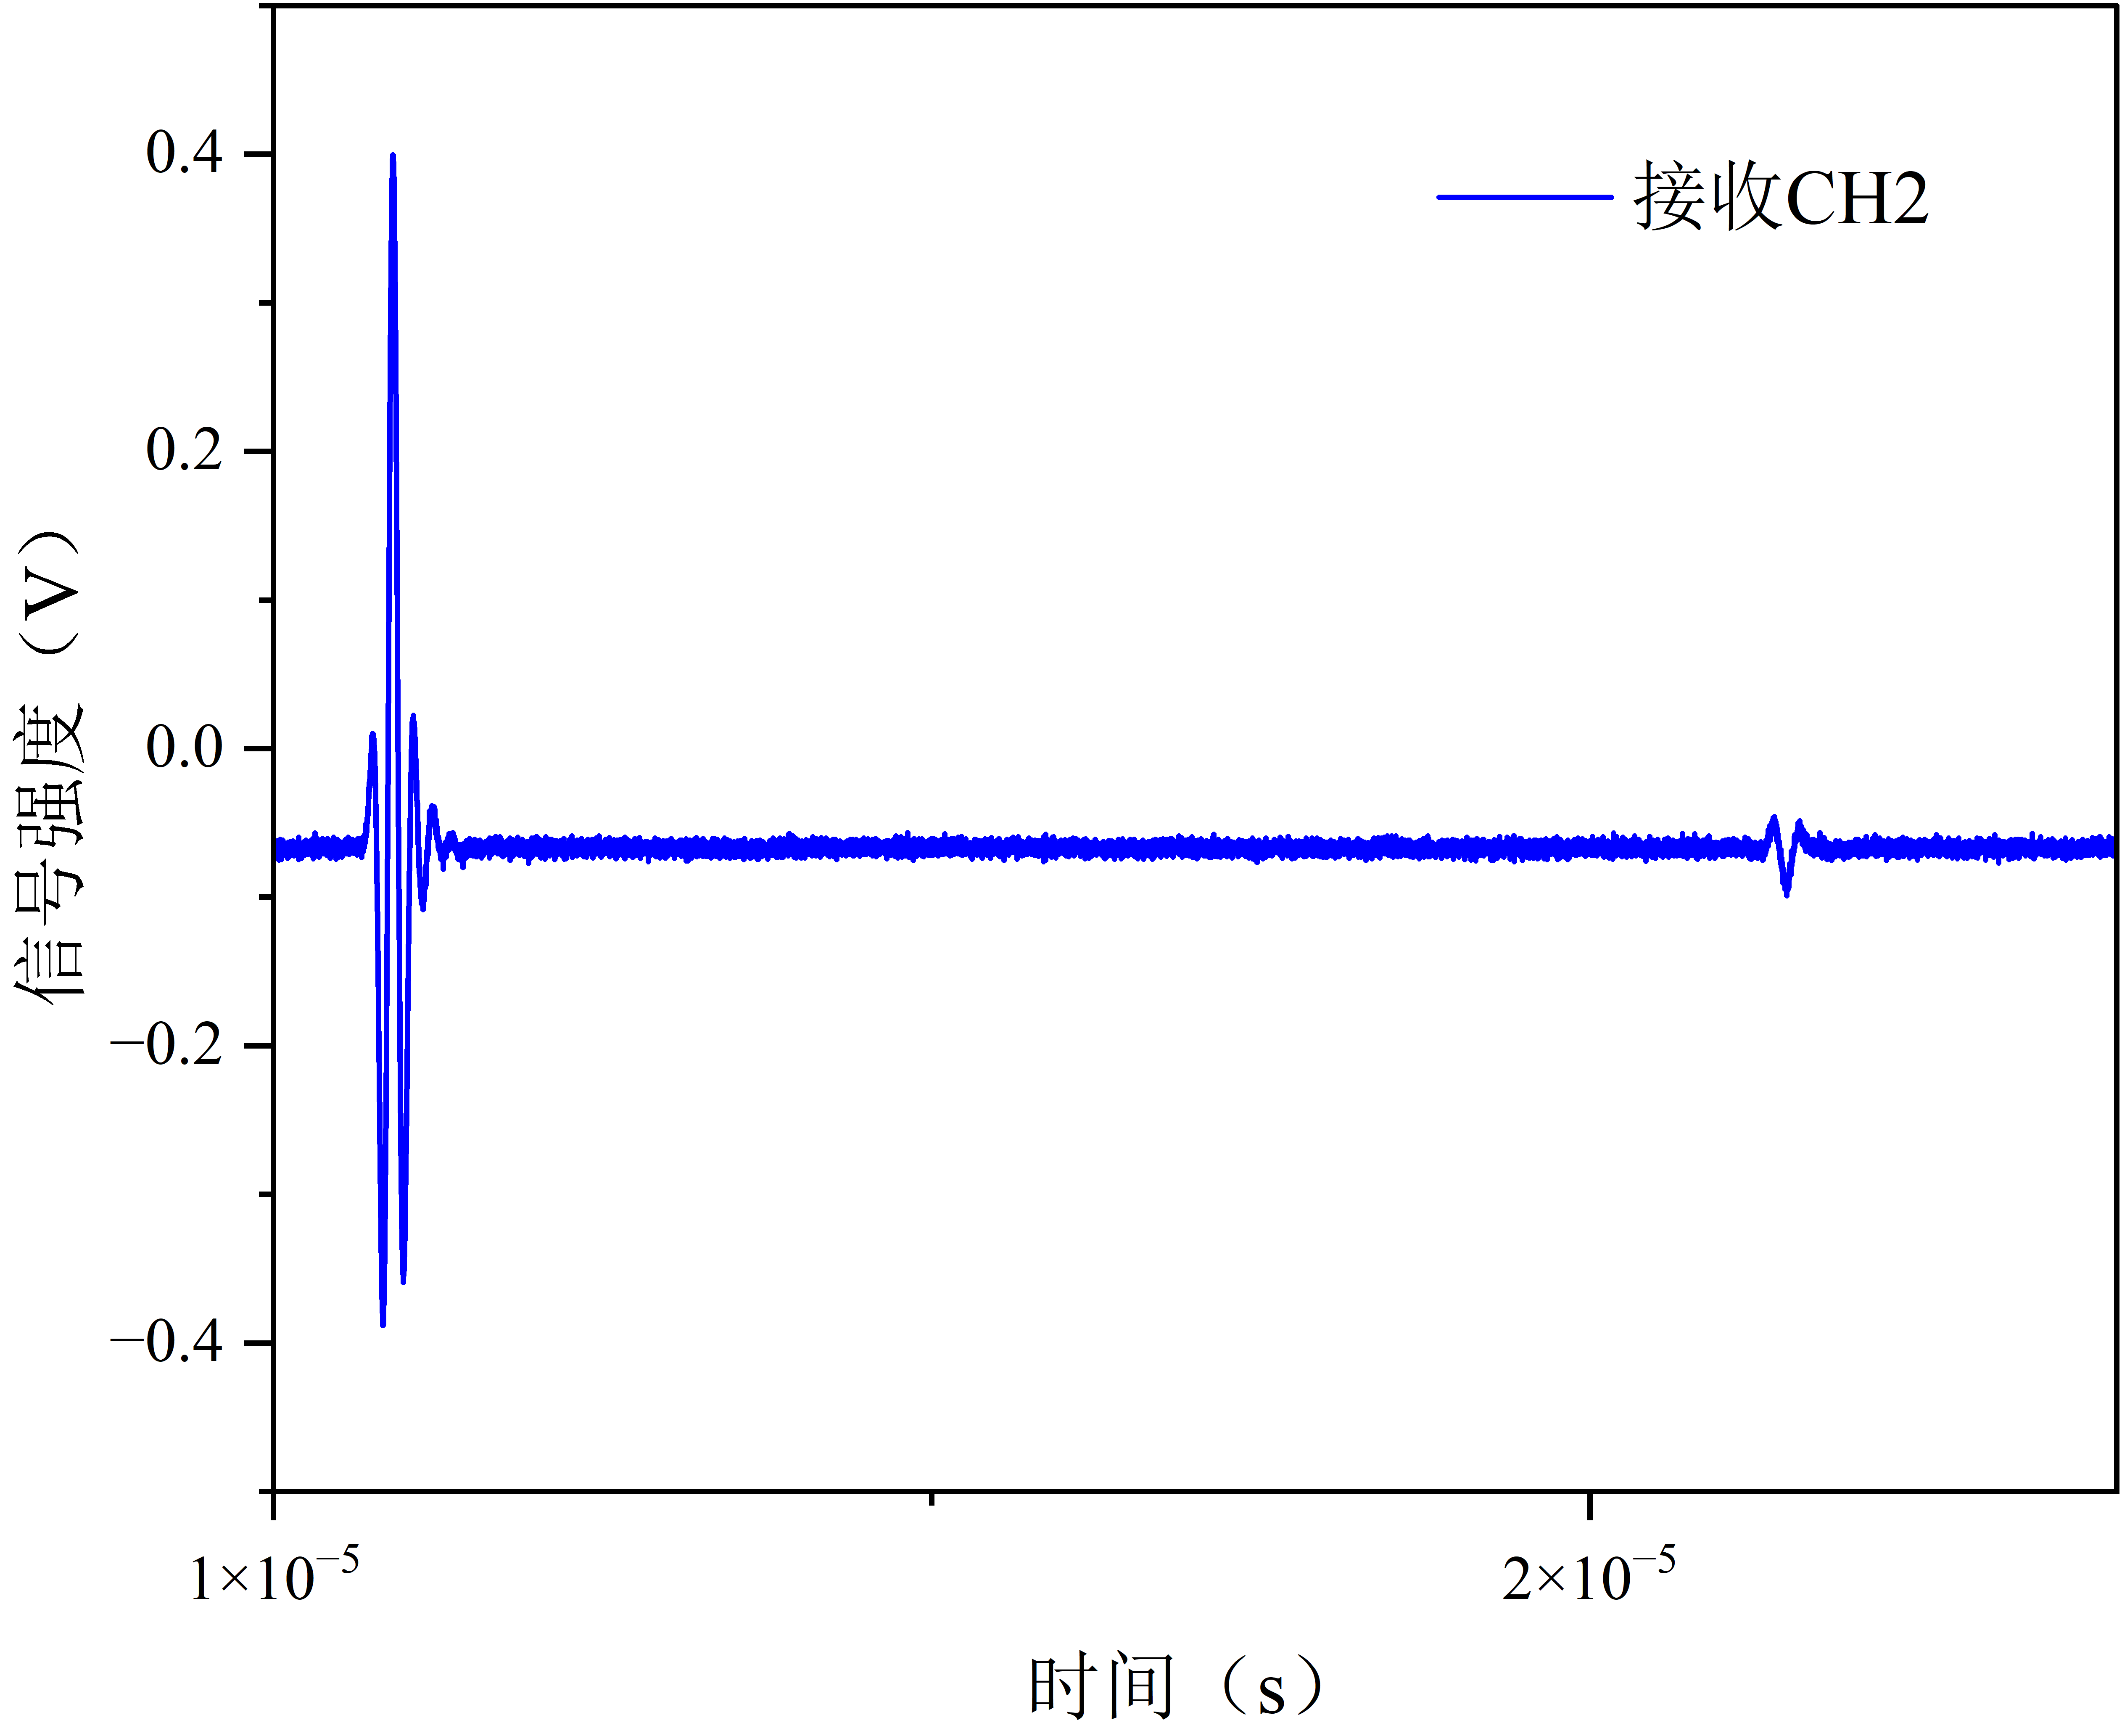
\includegraphics[width=\linewidth]{p16_img02.png}}
\caption{10 MHz 接触式测量有机玻璃试件纵波波速时信号图}
\label{fig:exp2-og-10}
\end{figure}

\begin{table}[H]
\centering\small
\caption{5 MHz 与 10 MHz 接触式测量有机玻璃中纵波波峰及衰减系数}
\label{tab:exp2-frequency-attenuation}
\setlength{\tabcolsep}{3pt}
\begin{tabular}{lcccc}
\toprule
测量对象及频率 & $P_m$（V） & $P_n$（V） & $\bar{\alpha}$（dB/cm） & $u(\alpha)$（dB/cm）\\
\midrule
有机玻璃 5 MHz & \blank[1.1cm]\ ($m=$\blank[0.4cm]) & \blank[1.1cm]\ ($n=$\blank[0.4cm]) & \blank[1.1cm] & \blank[1.1cm]\\
有机玻璃 10 MHz & \blank[1.1cm]\ ($m=$\blank[0.4cm]) & \blank[1.1cm]\ ($n=$\blank[0.4cm]) & \blank[1.1cm] & \blank[1.1cm]\\
\bottomrule
\end{tabular}
\end{table}

两种频率纵波在有机玻璃中的平均衰减系数为
\begin{subequations}
\begin{align}
  \alpha_{L,og}^{5\mathrm{MHz}}&=(\blank[1.4cm]\pm\blank[1.2cm])\ \mathrm{dB/cm},\\
  \alpha_{L,og}^{10\mathrm{MHz}}&=(\blank[1.4cm]\pm\blank[1.2cm])\ \mathrm{dB/cm}.
\end{align}
\end{subequations}
将本结果与水浸法结果比较，讨论低能量波峰、非零背景波、波峰选择和耦合剂均匀程度对衰减系数的影响。
\answer

\section{采用脉冲回波法确定焊缝钢板中缺陷的位置及大小}
实验钢板尺寸为 $30\times30\,\mathrm{cm}^2$。首先在钢板表面绘制网格线，便于探头扫描点定位。在钢板表面涂抹适量纵波耦合剂，每次间隔 1 cm 进行 B-Scan；为提高精度，当扫描结果显示存在缺陷时改为每隔 0.5 cm 扫描一次并记录结果。

\subsection{钢板侧面垂直入射}
从钢板没有焊缝的侧面采用 5 MHz 纵波探头进行探测，本组信号增益为\blank[2cm]。当扫描路径上存在缺陷时，探头激励的超声波将提前被缺陷反射，在波形图中产生异常回波信号。记录缺陷反射主要出现的时间区间：\blank[3cm]。在该区间取反射波形波峰和波谷对应信号强度绝对值中的最大值，作为该位置缺陷大小的度量，并绘制缺陷大小随位置变化的图线。

\begin{figure}[H]
\centering
\subcaptionbox{信号三维立体图}[0.48\textwidth]{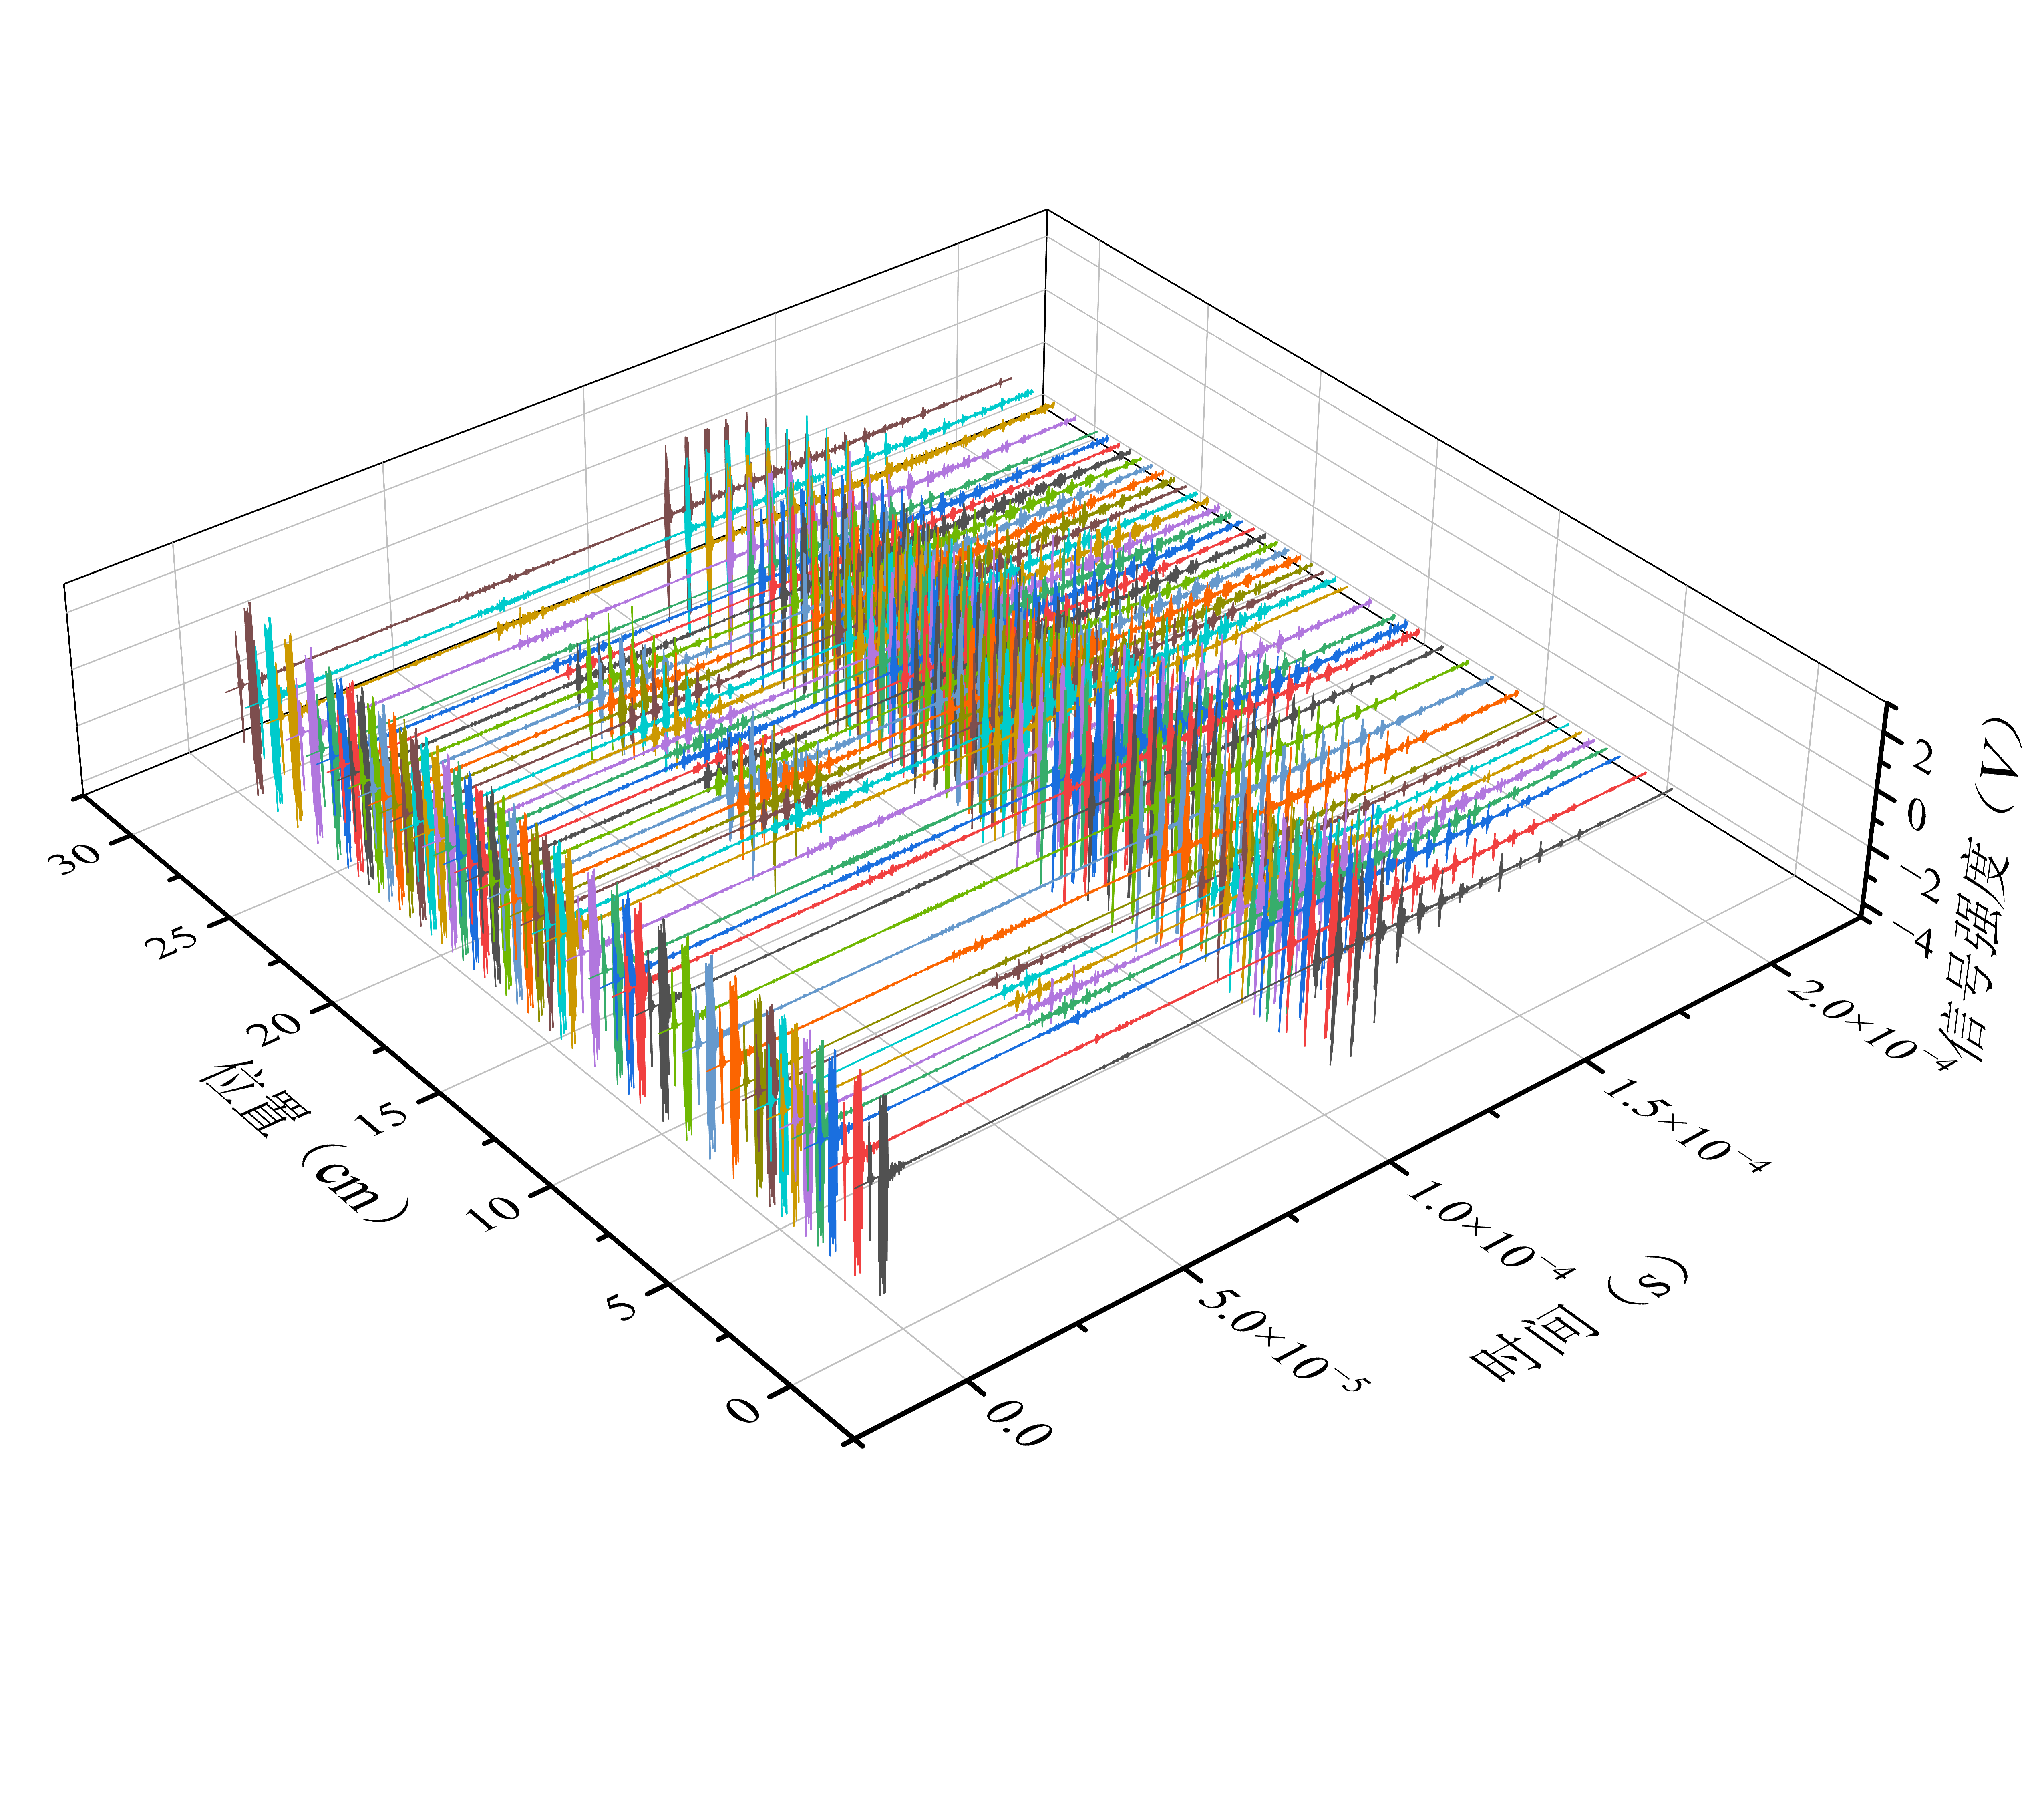
\includegraphics[width=\linewidth]{p17_img01.png}}\hfill
\subcaptionbox{损伤示意图}[0.48\textwidth]{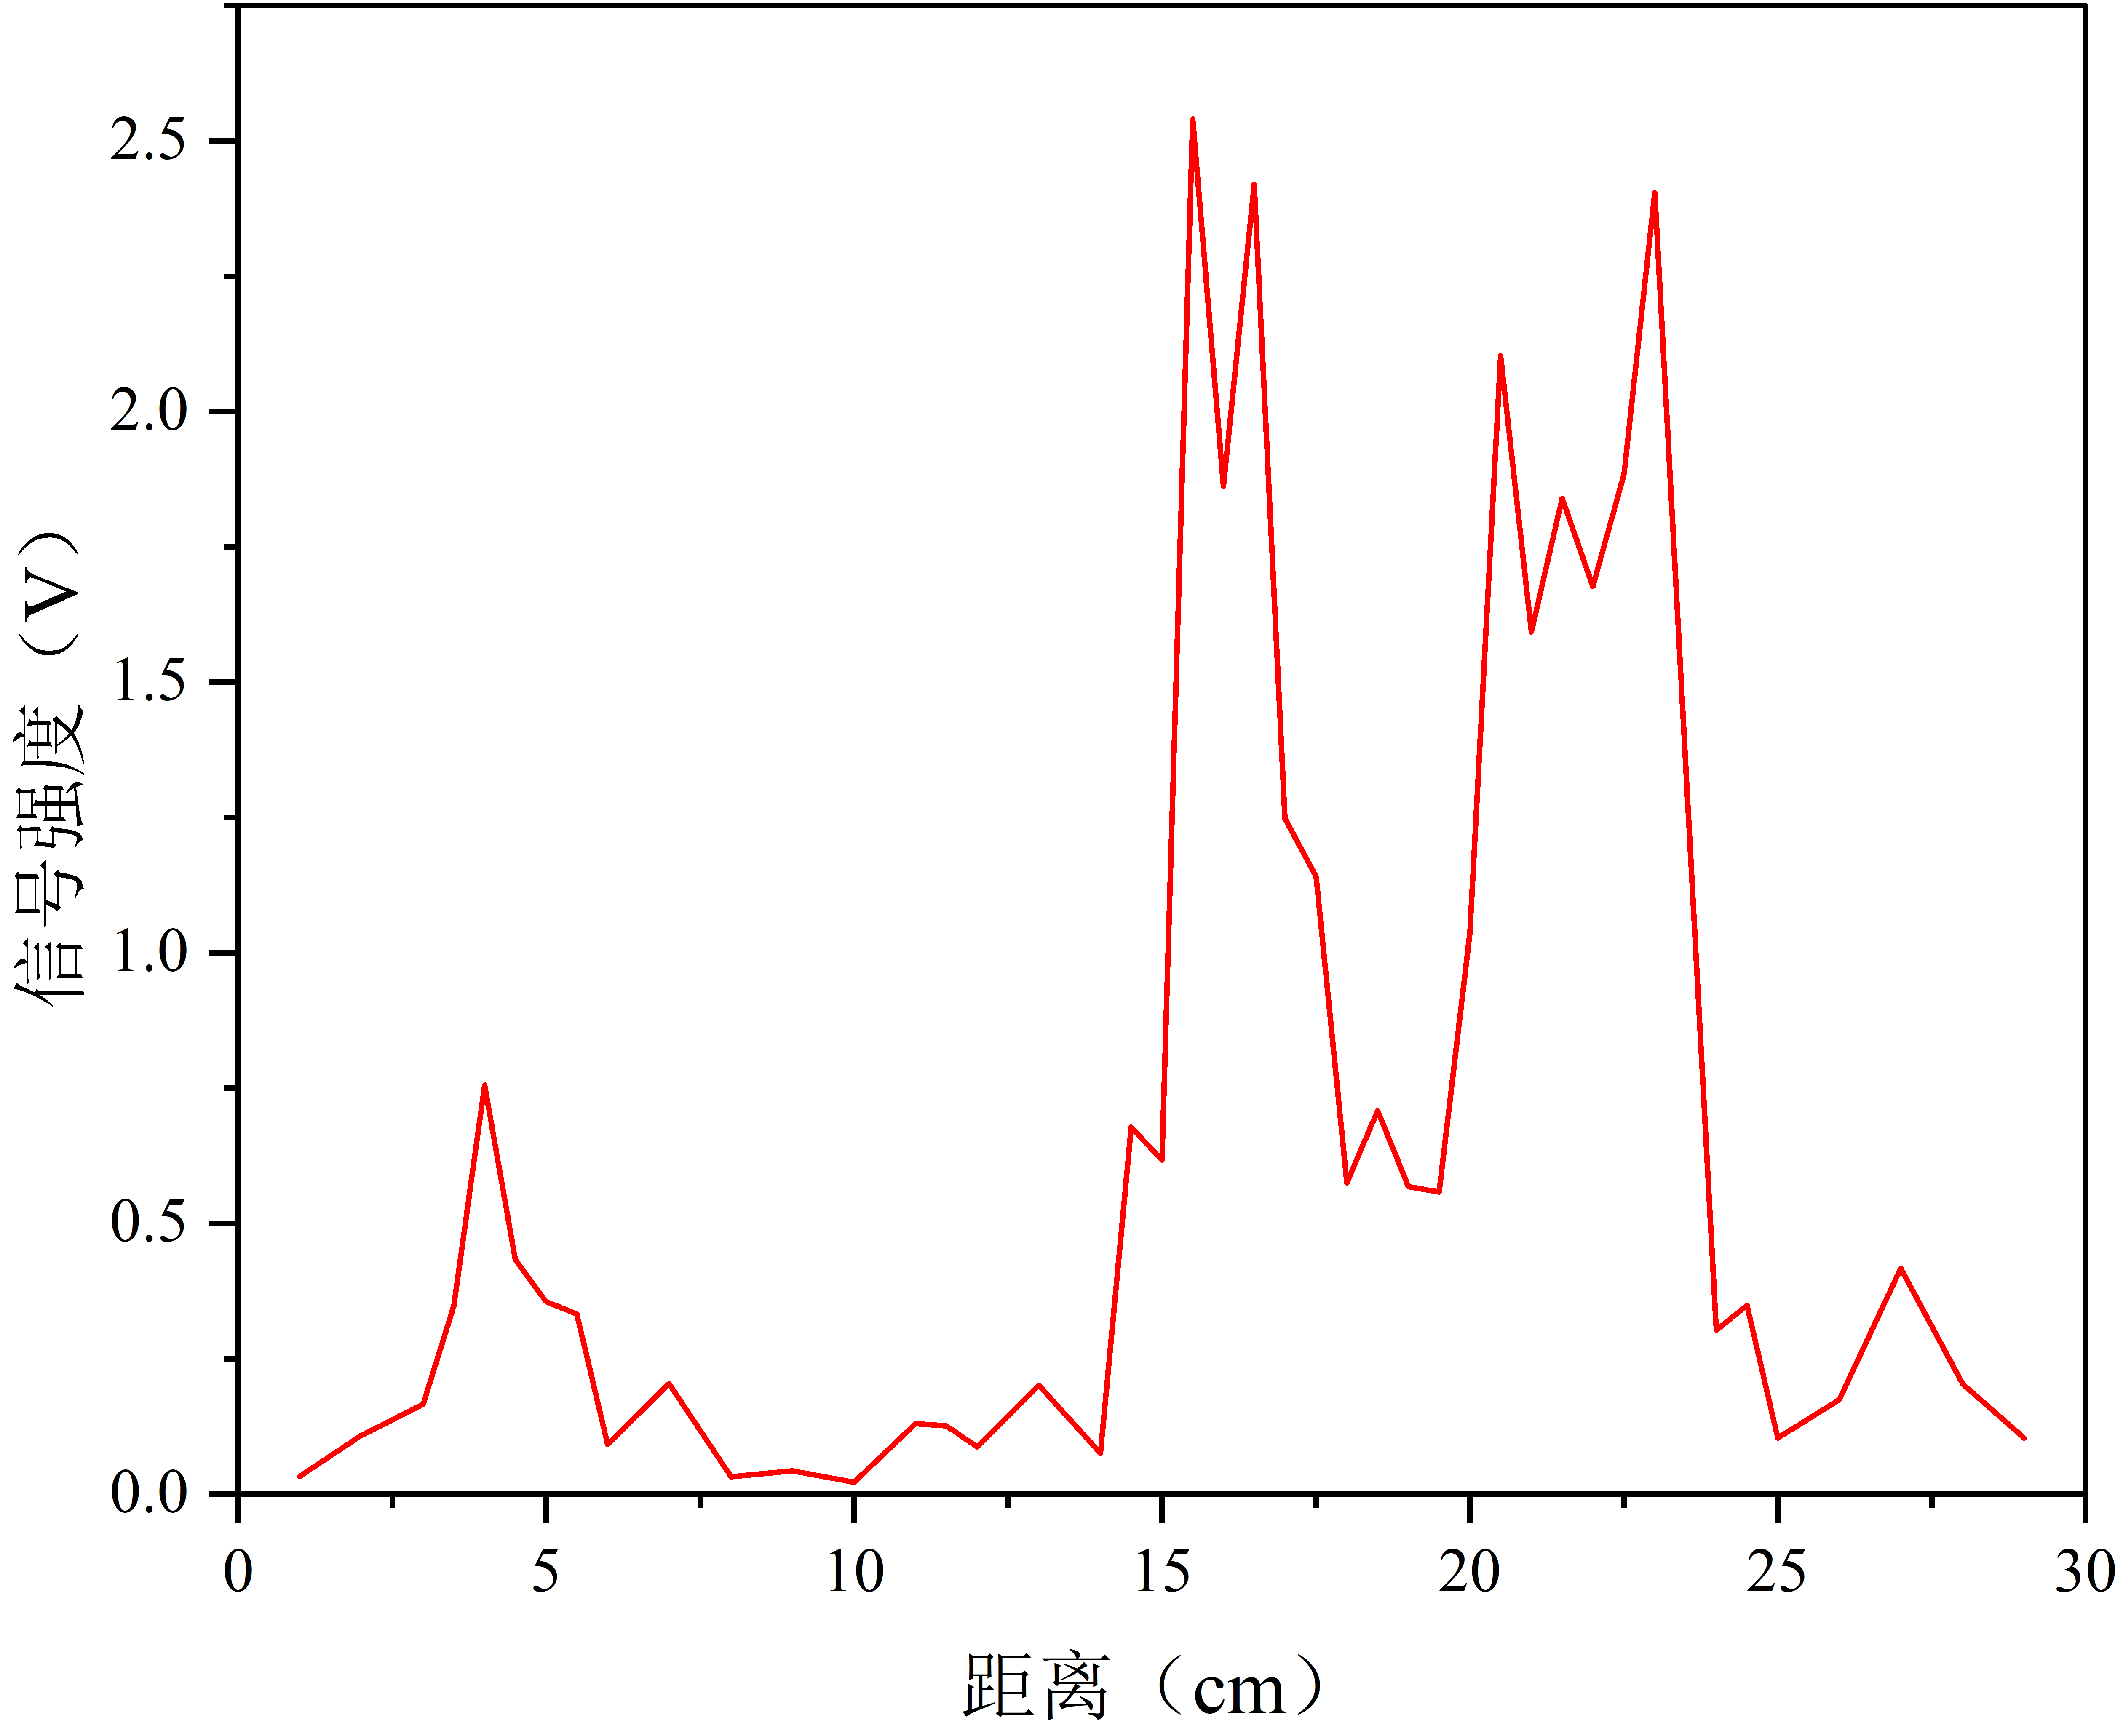
\includegraphics[width=\linewidth]{p17_img02.png}}
\caption{5 MHz 接触式纵波直探头测钢板焊缝（请替换为本组图像）}
\end{figure}
\noindent 缺陷位置与长度判断：\blank[0.72\textwidth]

\subsection{钢板表面斜入射}
在钢板有焊缝的表面采用 1 MHz 斜探头进行探测，本组信号增益为\blank[2cm]，斜探头倾角为\blank[2cm]。记录缺陷反射主要出现的时间区间：\blank[3cm]。按同样方法提取各位置缺陷反射强度并绘制损伤示意图。

\begin{figure}[H]
\centering
\subcaptionbox{信号三维立体图}[0.48\textwidth]{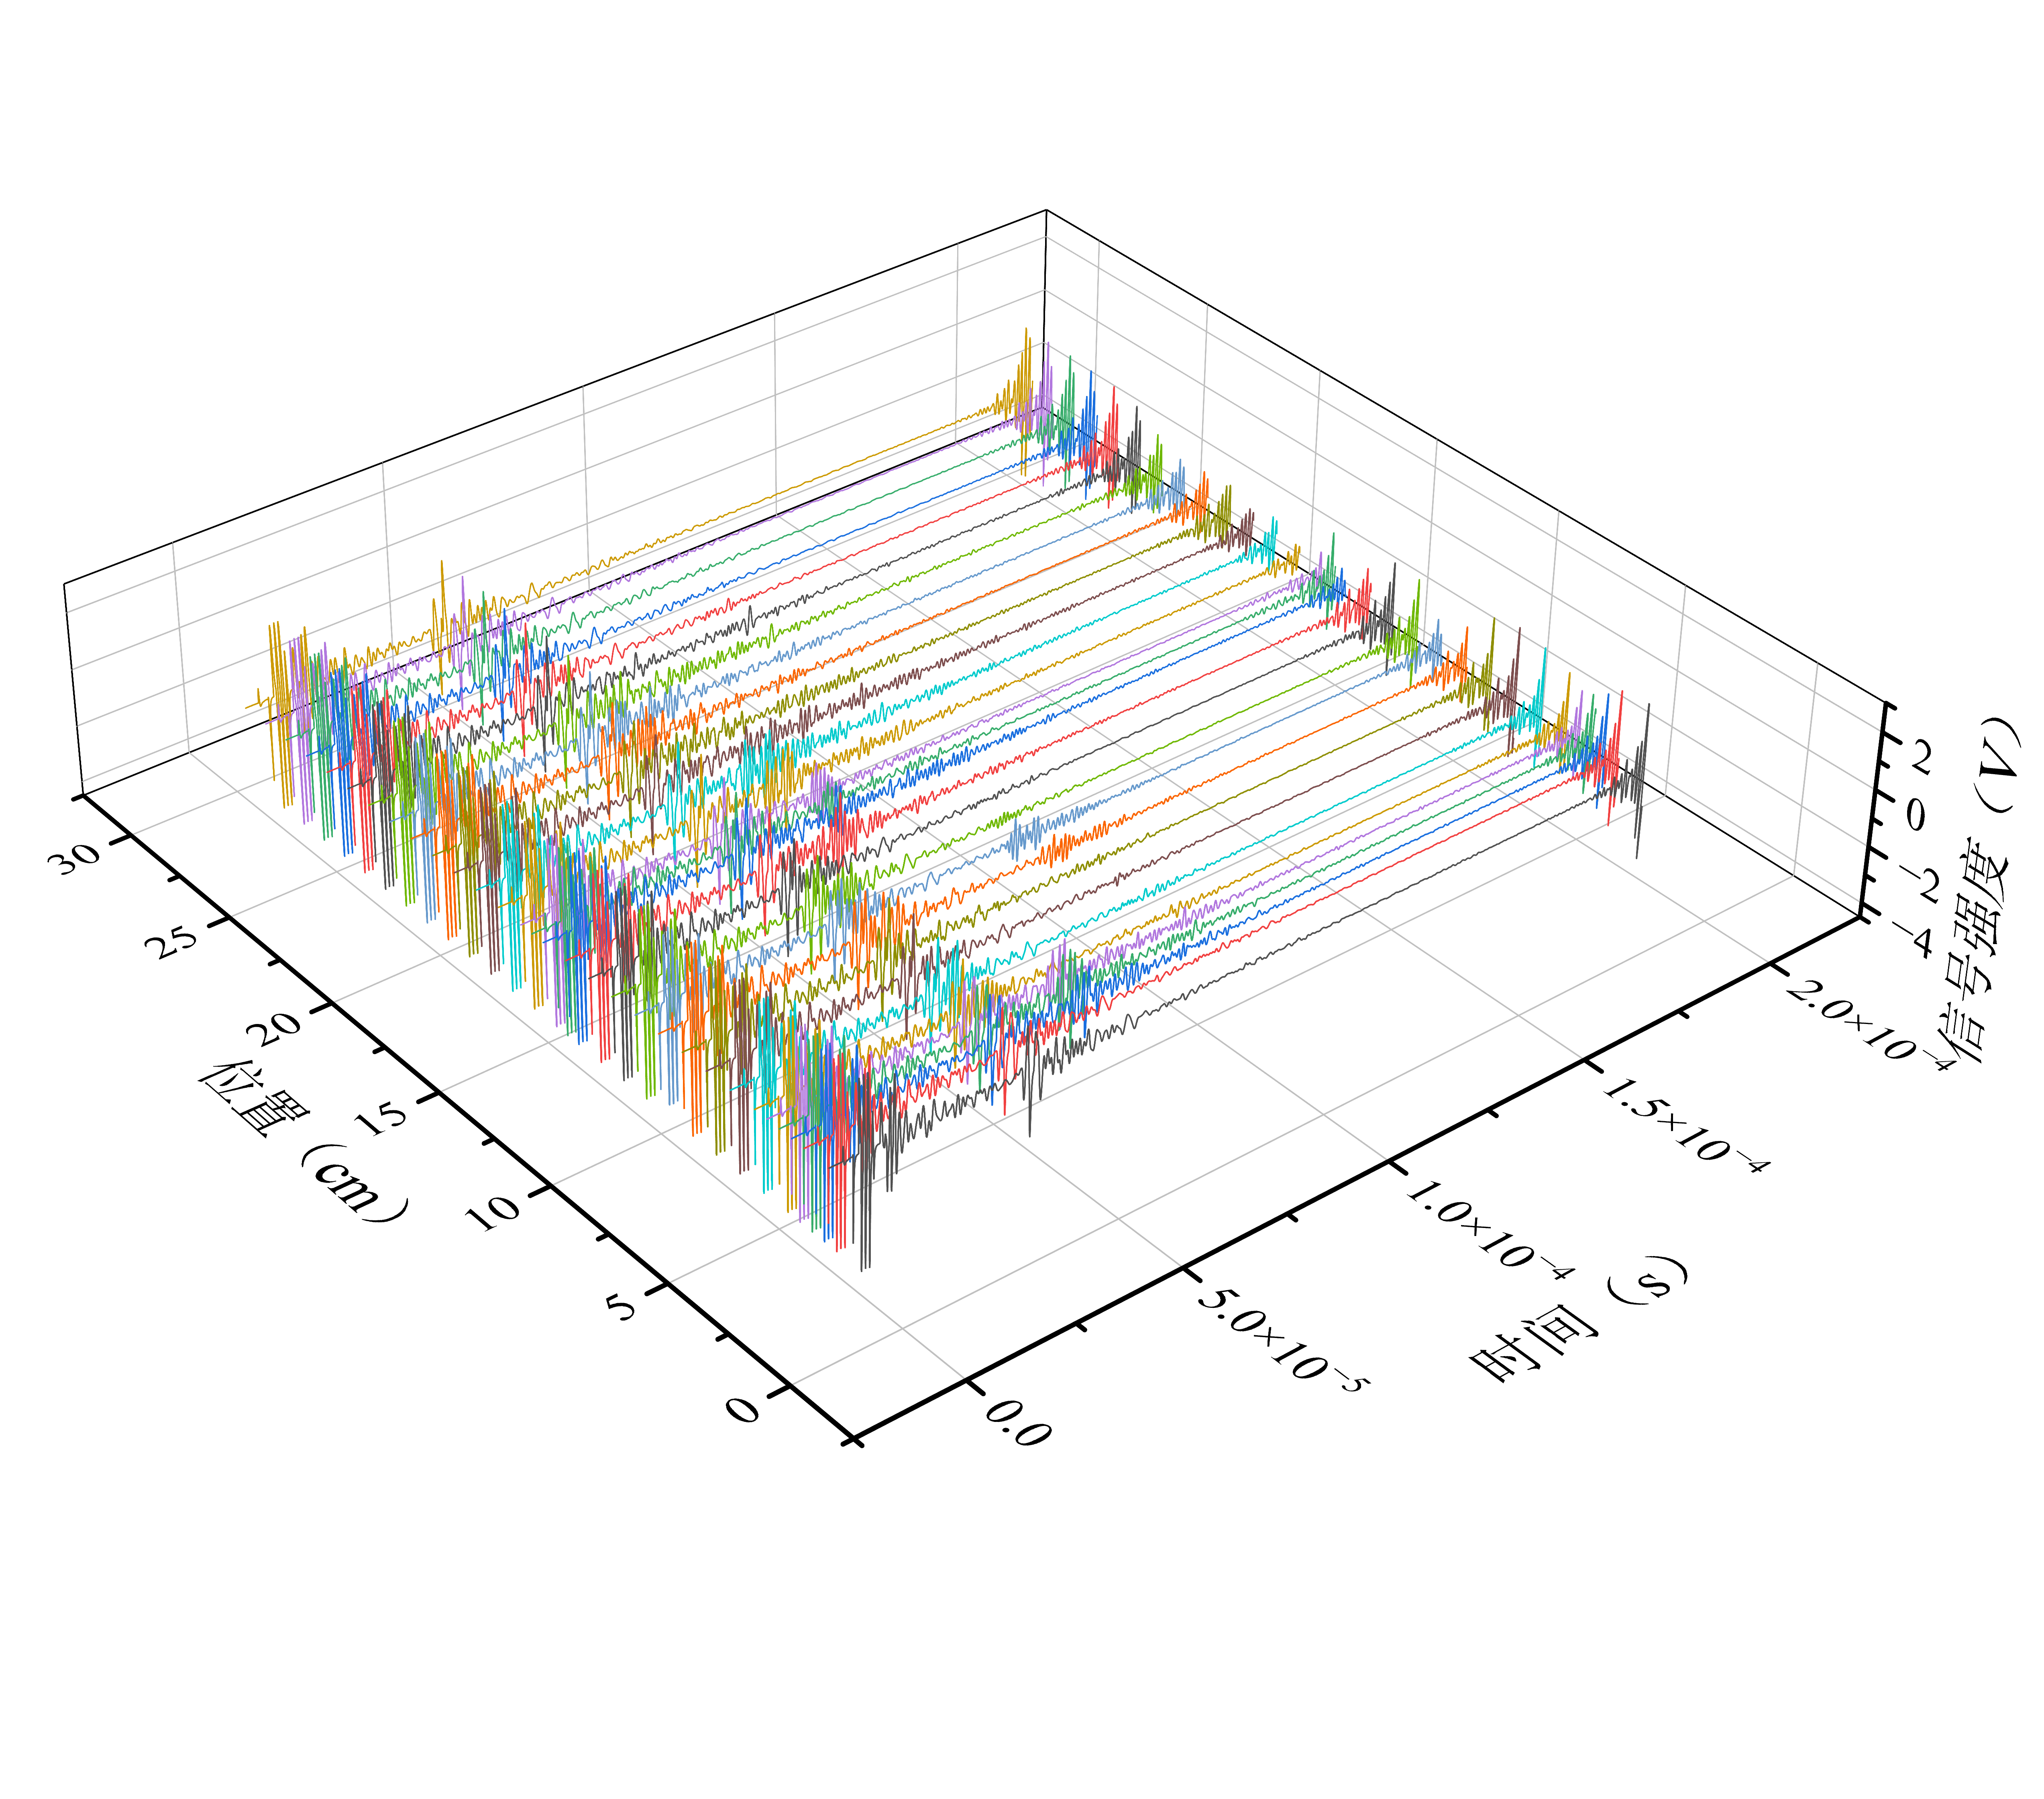
\includegraphics[width=\linewidth]{p17_img03.png}}\hfill
\subcaptionbox{损伤示意图}[0.48\textwidth]{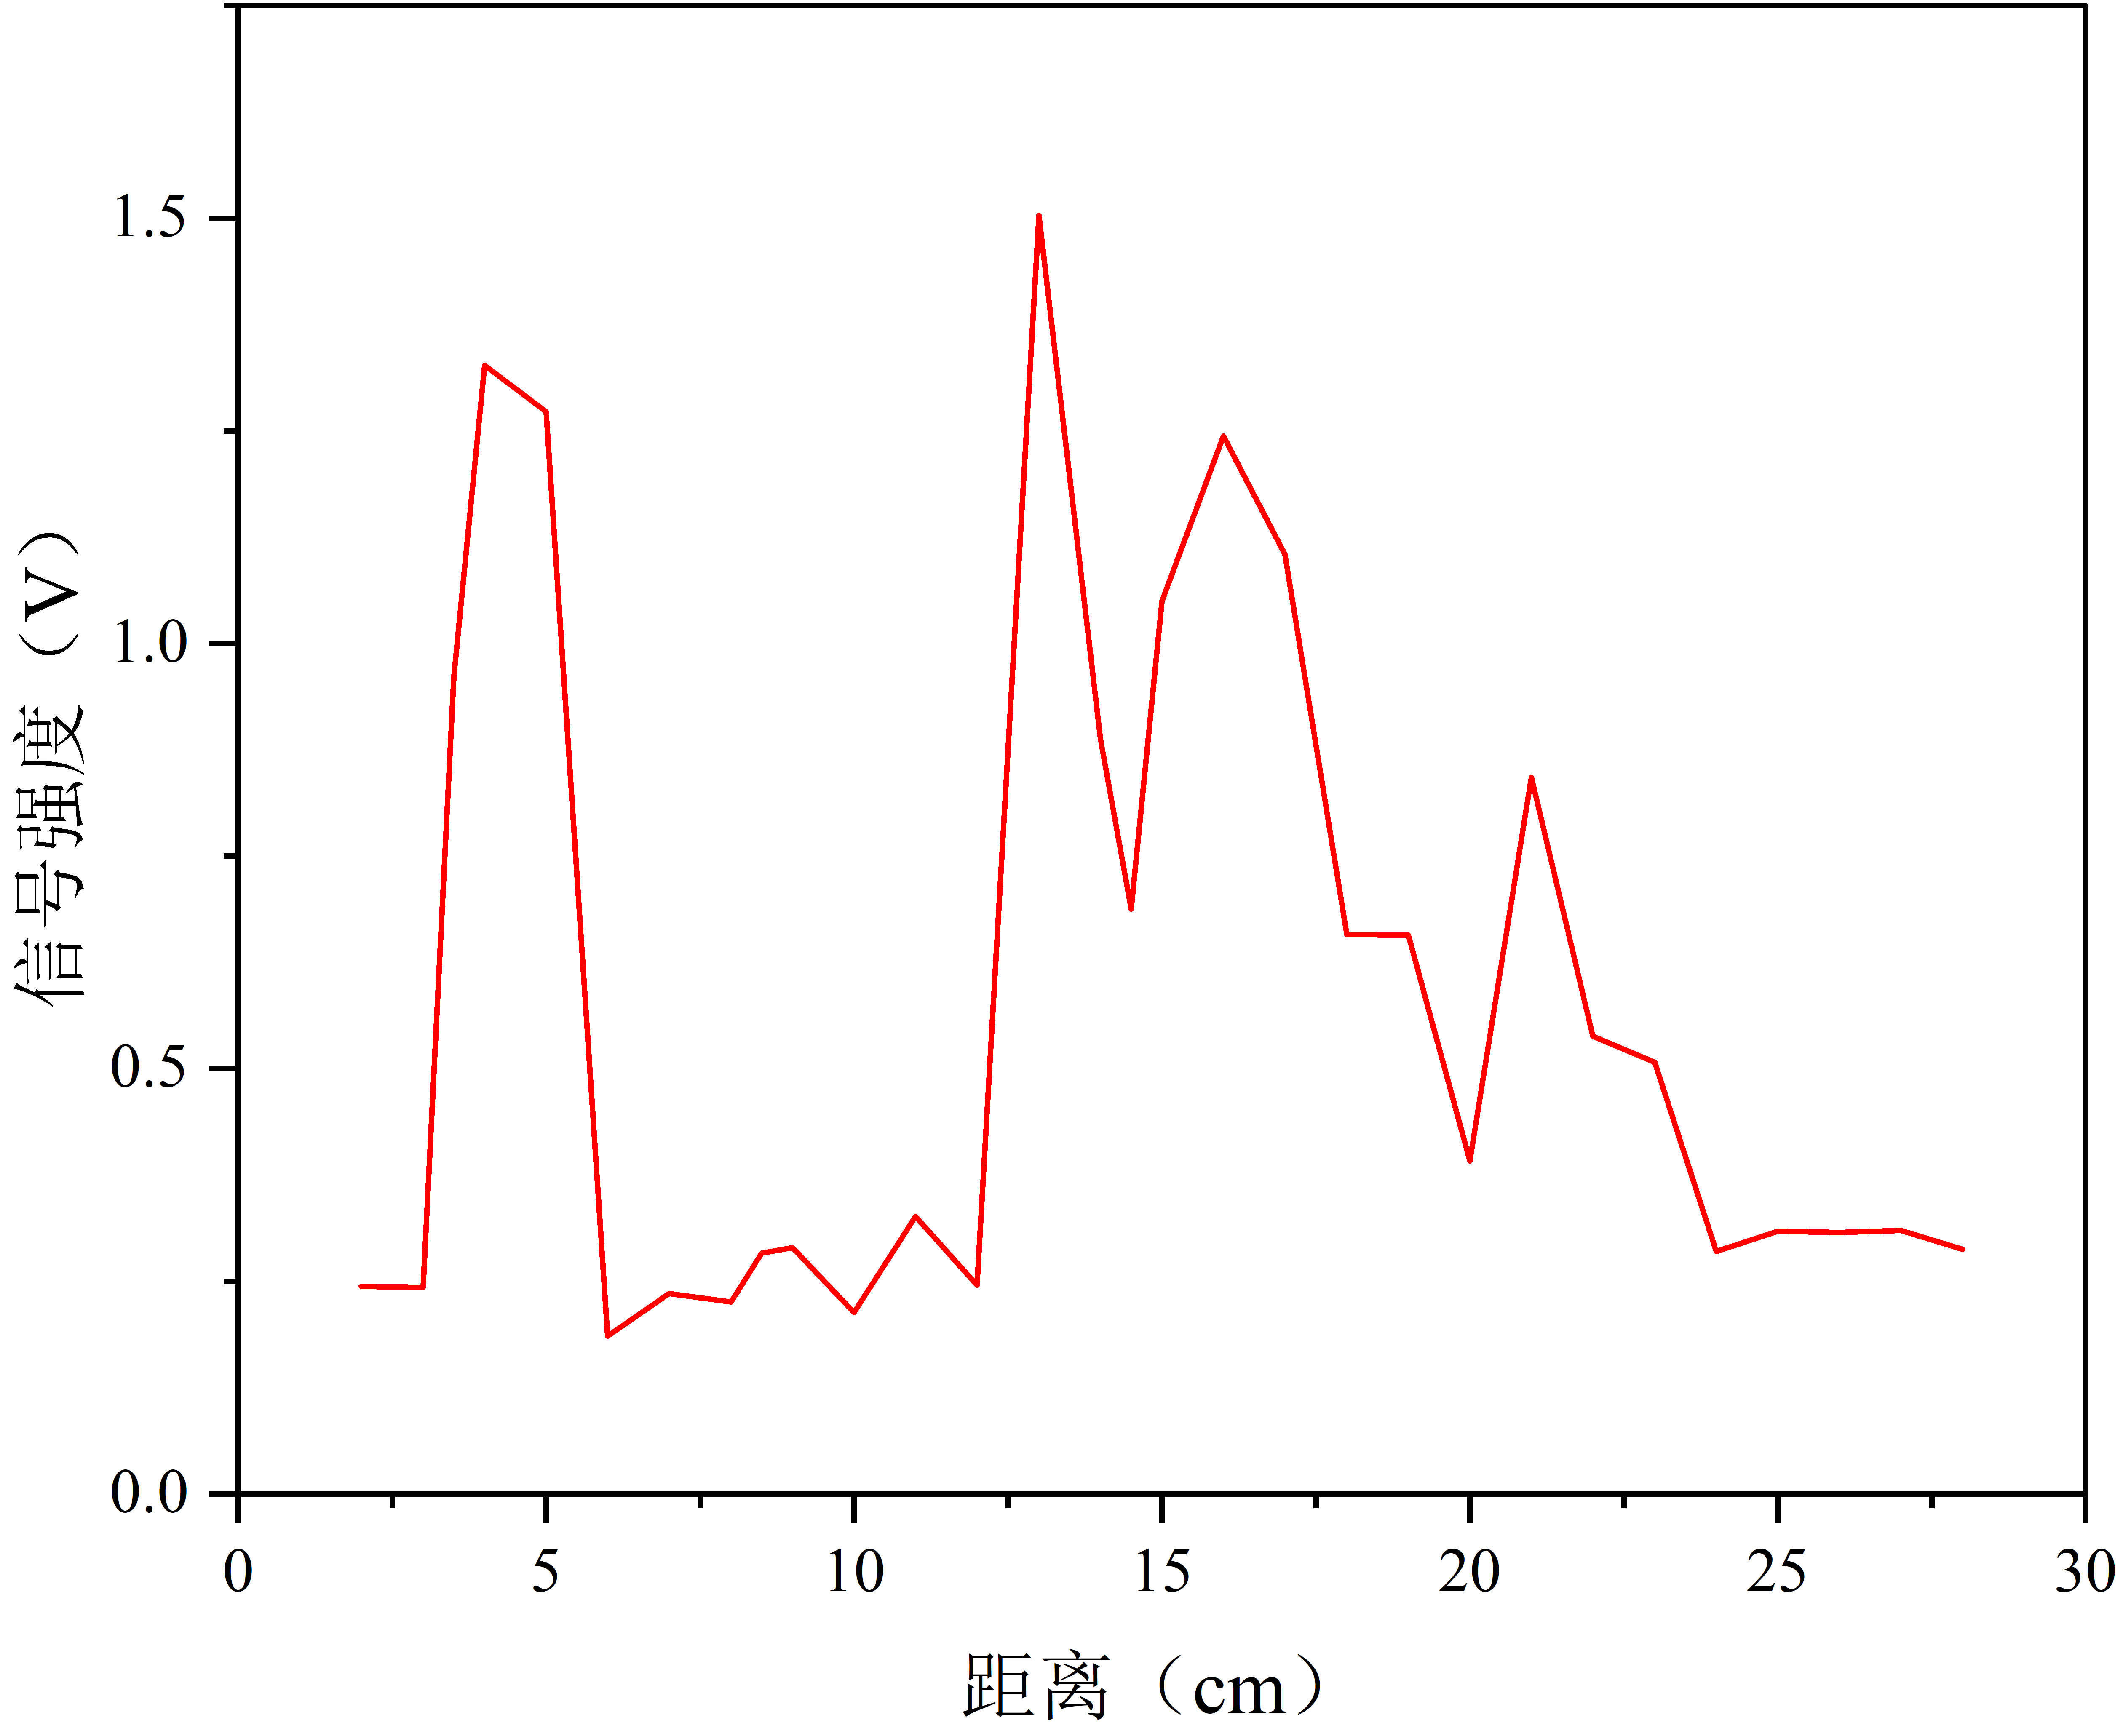
\includegraphics[width=\linewidth]{p17_img04.png}}
\caption{1 MHz 接触式纵波斜探头测钢板焊缝（请替换为本组图像）}
\end{figure}
\noindent 缺陷位置与长度判断：\blank[0.72\textwidth]

比较两种探头在同一裂纹处所得的相对反射能量及缺陷识别结果，并分析探测角度对结果的影响。
\answer

\section{结果分析与讨论}
\begin{enumerate}
  \item 比较三种试件的纵波、横波波速及纵波衰减系数，并结合材料微观结构进行解释。声波在固体材料中传播时，其传播速度和能量传递效率与材料微观结构密切相关。金属材料如钢和铝在微观上主要由紧密排列的金属离子组成，周围有大量自由电子运动，这一结构赋予金属较高的密度和刚度。根据振动力学理论，较高的密度和刚度通常会提升声波传播速度并增强能量传递效率。相比之下，有机高分子材料由于分子间作用力较弱、密度较低、刚度较小，其分子链具有较强柔性，微观结构周期性弱，导致波在传播过程中发生更大的能量耗散，使其宏观表现出更低的波速和更大的衰减系数。
  \item 不同频率的超声探头各自具有优势与不足。频率较高的探头有利于发现更小的缺陷，且脉冲宽度小、分辨力高，有利于区分相邻缺陷；其波长短，半扩散角小，声束指向性好，能量集中，有利于发现缺陷并对缺陷定位。不利因素包括近场区长度大、随频率增加衰减急剧增加，并且对材料非均质性较敏感。因此，探头选择应根据具体实验需求，一般在保证检测灵敏度的前提下尽可能选用较低的频率。
  \item 在使用水浸法测量有机玻璃时，若波形图中出现较多非上下表面的回波，可分析探头是否做到完全垂直入射，以及部分波是否经过水面和底面反射造成噪音。
  \item 使用接触法测量金属试件时，若波形图中存在类似波包的结构，可考虑理想探测工况为无限大板，而实验室使用圆柱体，边界处可能发生波的反射甚至共振。
  \item 在缺陷探测中，两种探头在同一裂纹处所得的相对反射能量可能不同，因为两者对缺陷的探测角度不同。可根据这一点大致推断裂纹形状，并比较斜探头与直探头的测量结果。
\end{enumerate}
结合本组数据，补充结果分析与讨论。
\answer

\section{数据误差分析与提高精度的方法}
\begin{enumerate}
  \item 测量纵波与横波速度时，有机玻璃的波速误差可能源于材料本身的非均匀性以及探头与试件的贴合程度。有机玻璃信号强度整体偏弱时，判断波峰之间时间差也会产生误差，可尝试通过增加增益改善测量。
  \item 通过不同方法（水浸法与接触法）测量钢和有机玻璃的纵波速度，可以比较测量方法及探头频率对结果的影响。有机玻璃衰减系数在不同方法下可能存在较大差异，原因包括材料耗散明显、靠后波峰能量小、取值容易受到非零背景波影响。应选择合适的波峰和数据处理方式，并保证耦合剂涂抹均匀。
  \item 进行衰减系数计算时，如果只选取两个时刻的波峰，较少的数据点容易产生较大误差。为提高精度，可以对原始公式取对数，进而拟合直线，通过斜率计算衰减系数。
  \item 剩余误差主要来源于多次测量的读数误差以及仪器固有误差，可以通过提高测量精度、优化实验操作来减小误差。
\end{enumerate}
结合本组实际操作，补充具体误差来源与改进措施。
\answer

\end{document}
